% !TeX spellcheck = en_US



\section{Lipids}

In the previous chapter, the method of using a sacrificial layer to detach ice is discussed. For this, lipids need to be solved at cryogenic temperatures. As not every lipid is solvable in all solvents, an experiment is conducted to obtain solvents at room temperature. then the best solvents are tested at cryogenic temperatures.

The solubility of lipids at room temperature in different solvents are determined. For this experiment the cover glasses are coated with lipids. Then a first reference image was taken. Then the cover glass is given into a small container with the potential solvent. After 15 minutes, the cover glass is removed and compared under the microscope with the reference picture. If streaks created from lipids are still as visible as before, the lipids are categorized as insoluble in this solvent. If the streaks partially dissapeared and/or are less visible, the lipids are categorized as partially soluble in this solvent. Last if the streaks completely disappear, the lipids are assinged as soluble in the solvent (Table \ref{table:LoeslichkeitRaumtemperatur}).

\begin{figure}[hbt!]
	\centering
	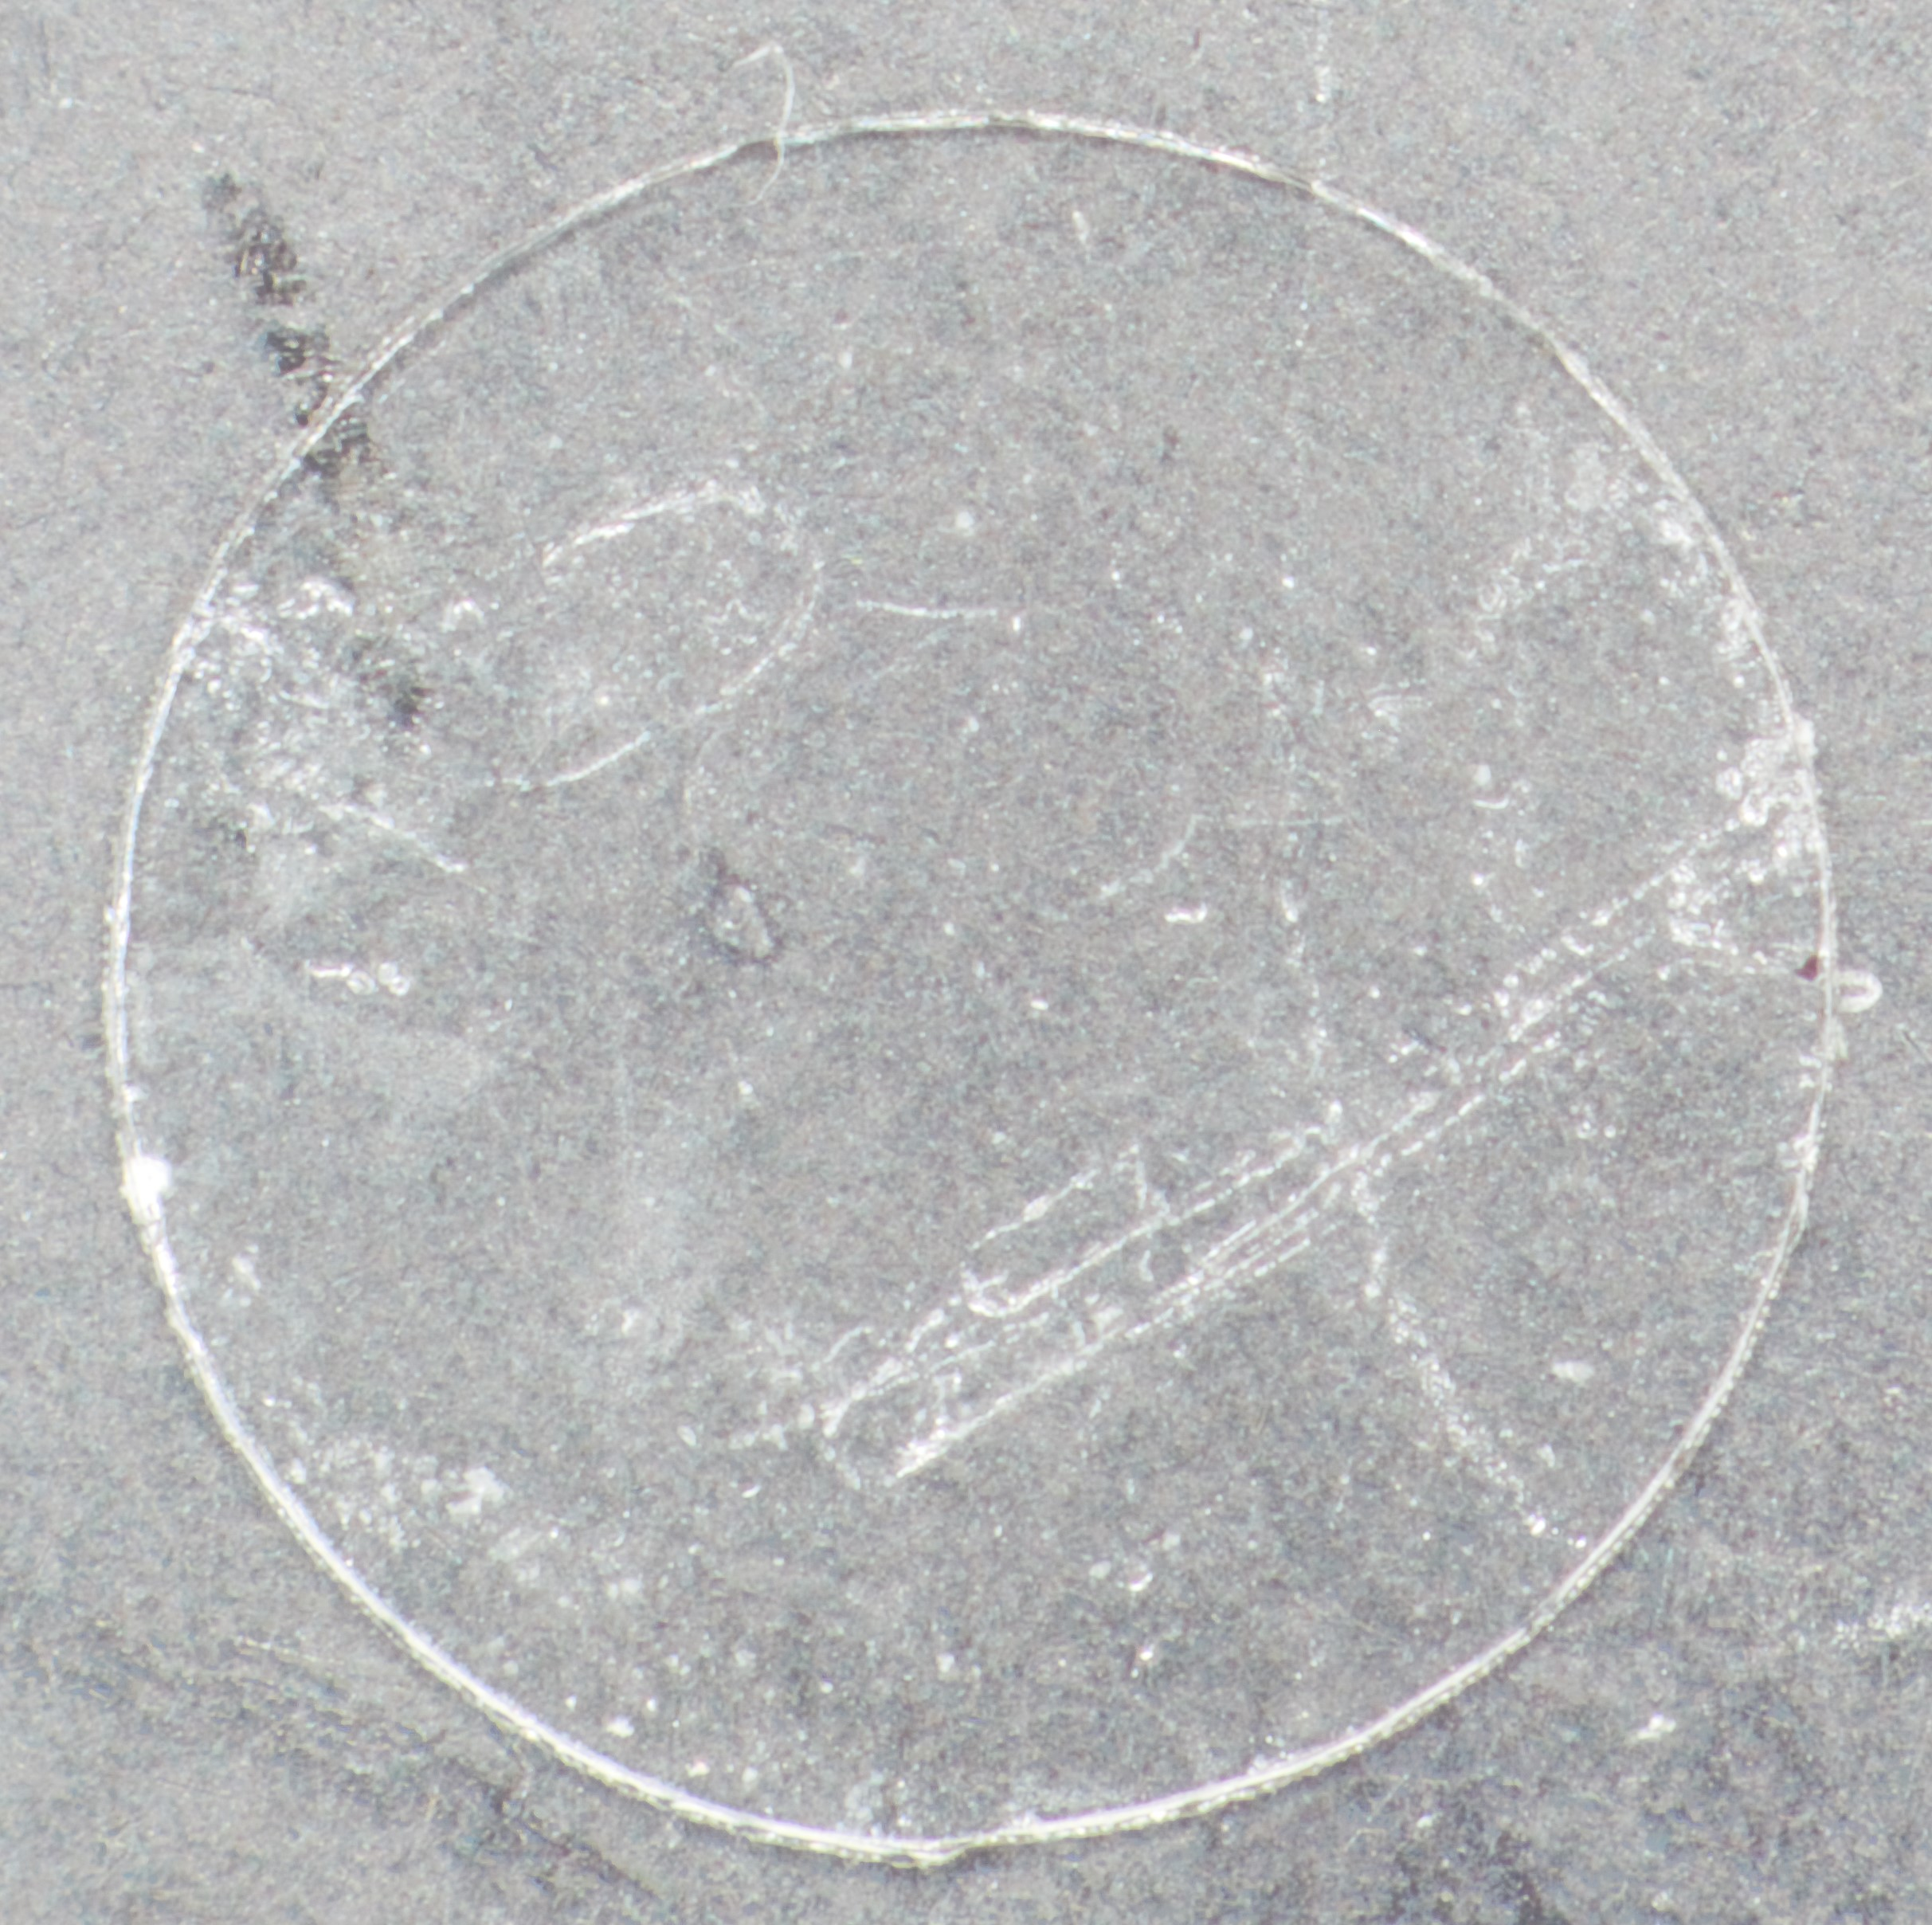
\includegraphics[width=7cm]{SlideWIthLipidStreaks.jpg}
	\caption{Example of a $\varnothing$\SI{5}{\milli\meter} cover glass with lipid residuals on the surface.}
\end{figure}


\begin{table}[hbt!]
	\centering
	\begin{tabular}{|l|c|c|}
		\hline
		potential solvent & solubility EGG-PC & solubility DOPC \\
		\hline
		\hline
		4-Methyl Pentene & soluble & N/A  \\ 
		\hline
		3-Methyl Pentene & slightly soluble & insoluble \\
		\hline
		1-Pentene & insoluble & insoluble \\
		\hline
		Isopentane & soluble & slightly soluble\\
		\hline
		1-Propanol & soluble & soluble\\
		\hline
		Pentane & soluble & insoluble\\
		\hline
		Ethanol & N/A & soluble\\
		\hline
	\end{tabular}
	\caption{Result of solubility tests at room temperature. Soluble indicates solvents which are able to visibly solve all lipids off a cover glass. slightly soluble indicates solutions which are able to solve lipids with residuals. Insoluble indicates no visible removal of tested lipid.}
	\label{table:LoeslichkeitRaumtemperatur}
\end{table}

This experiment shows that each three different solvent exist for EGG-PC and DOPC with high solubility (Table \ref{table:LoeslichkeitRaumtemperatur}). Following these results, solvents categorized with "soluble" are tested regarding solubility at temperatures of \SI{-140}{\degreeCelsius}. As not all solutions are liquid at \SI{-140}{\degreeCelsius} (Table \ref{table:SchmelztemperaturLösungsmittel}), they are tested at higher temperatures above their melting point, as mentioned in chapter \ref{chapter:meltingtemp}. In addition they are tested as mixtures with other solvents with a lower melting point. Additionally liquid ethane is tested as solvent. Ethane was not tested at room temperature, as the boiling point is at \SI{-88.6}{\degreeCelsius} \cite{PubChem.29.08.2023}.

In the experiment, no tested solvent was able to completely solve lipids at \SI{-140}{\degreeCelsius} and within \SI{15}{\minute} (Table \ref{table:Cryoloeslichkeit}). Also streaks of applied lipids did not only stay partially behind, but also new streaks appear on the glass slides. This means that some lipids redistributed on the same glass slide.

Using solvents to remove a sacrificial layer, a high solubility is required. In practice, the sacrificial layer is completely covered by the ice layer except the edges. Therefore area of contact with the solvent is small, slowing the process considerably. Additionally, as the ice layer needs to stay vitrified. The temperature cannot be raised over \SI{-140}{\degreeCelsius} to speed up the process.

The solving process of lipids proves to be endothermic. This means that heat is needed to solve lipids, so cold temperature heavily decrease solubility QUELLE DENNIS ODER SO. This effect was observed over the last experiments by all solvents to varying degree. It can be assumed that the majority of solvent lipids mixtures are endothermic which is very disadvantageous for finding a potential solvent lipid candidate. Strongly exothermic solvents could heat up the ice enough to crystallize the ice. So weakly exothermic solvents would be optimal for this task.

\begin{table}[hbt!]
	\begin{subtable}{\linewidth}
		\centering
		\begin{tabular}{|l|l|}
		\hline
		Solvent & Result \\
		\hline
		\hline
		Pentane & soluble at \SI{-125}{\degreeCelsius} \\
		\hline
		4-methyl pentene & insoluble \\
		\hline
		\makecell[l]{1:1 volume ratio\\ HFE to 1-Propanol} & \makecell[l]{did not mix,\\ slightly soluble}\\
		\hline
		Liquid ethane & insoluble\\
		\hline
		\end{tabular}
		\caption{EGG-PC}
		\label{table:EGG-PCCryoloeslichkeit}
	\end{subtable}
	\begin{subtable}{\linewidth}
		\centering
		\begin{tabular}{|l|l|}
		\hline
		Solvent & Result \\
		\hline
		\hline
		\makecell[l]{1:4 volume ratio\\ 1:2 molar ratio\\ Ethanol to Isopentane} & slightly soluble\\
		\hline
		\makecell[l]{1:2 volume ratio\\ 1:1 molar ratio\\ 1-Propanol to Isopentane} & insoluble \\
		\hline
		Isopentane & slightly soluble\\
		\hline
		1-Propanol & \makecell[l]{at \SI{-130}{\degreeCelsius}\\ slightly soluble}\\
		\hline
		Liquid ethane & insoluble \\
		\hline
		\end{tabular}
		\caption{DOPC}
		\label{table:DOPCCryoloeslichkeit}
	\end{subtable}
	\caption{ in \ref{table:EGG-PCCryoloeslichkeit} for EGG-PC, no sufficient solubility at -140°C was found. In \ref{table:EGG-PCCryoloeslichkeit}, DOPC was tested but also no proper solution was found.}
	\label{table:Cryoloeslichkeit}
\end{table}

\FloatBarrier
\section{Detaching ice mechanically}
\label{Chapter:LipidPullingTests}

TODO

For this section, cover glass coated in Parylene are used as object slide. The slide is then dipped in solution containing lipids for a lipid coating. A ice layer with fluoriscine is frozen with either plunge-freezing or using a pincer and liquid nitrogen. Additionally, the "finger" is used as tool to try lifting off a piece of ice from the frozen layer on top of the lipids. In the next sections, different variables are examined and tested.

\subsection{Volume of Hydrofluorether}

First the volume of HFE is evaluated. High dosages of liquid HFE can spread underneath the frame holding the sample, leading to an inefficient force distribution. Also a thick glue layer take less tensile force, leading to a reduction of maximum force on the sample. Too little HFE will not connect the finger to the sample. Additionally, the dosaging of glue ia found to be a challenge.

The HFE is dosaged with a pipette onto the tip of the "finger". While pipetting, around \SI{4}{\micro\liter} of HFE is evaporating. Based on this knowledge, dosaging $4.10\,\mu l$, $4.30\,\mu l$ and $4.50\,\mu l$ is compared and a video is taken for later comparison.

The videos show that pipetting HFE is not reliable. The visible HFE volume on the tip does not correlate with the dosaged volume. On reason is a difference in the volume of HFE evaporating while applying. Also some HFE may be placed on the side of the tip. When using the finger, only the HFE on the flat tip is effective.

\begin{figure}[hbt!]
	\centering
	\begin{subfigure}[]{0.45\textwidth}
		\centering
		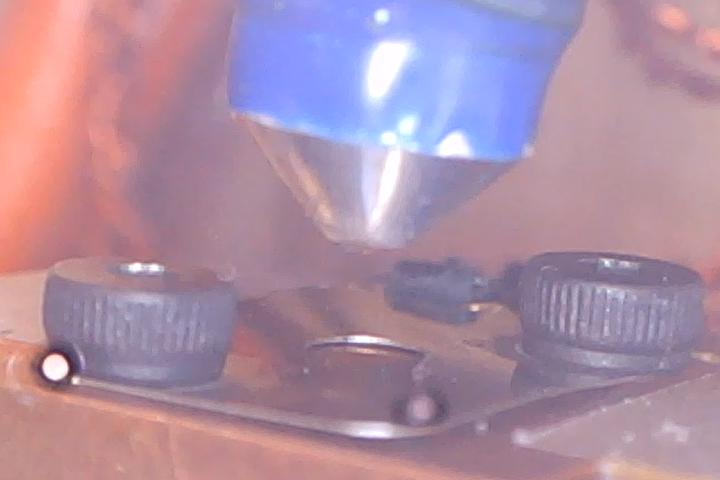
\includegraphics[width=7.5cm]{LowerLimit_quadrat}
		\caption{lower limit HFE volume}
	\end{subfigure}
	\begin{subfigure}[]{0.45\textwidth}
		\centering
		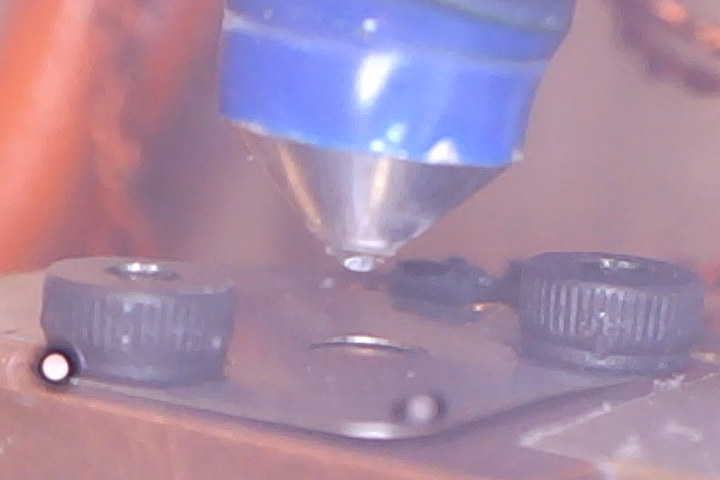
\includegraphics[width=7.5cm]{UpperLimit_quadrat}
		\caption{upper limit HFE volume}
	\end{subfigure}
	\caption{Visual representation of the range of dosages which are the most reliable. less HFE than the lower limit is more likely to not attach to the sample properly. more HFE than the upper limit will spread under the "window" brace or results in a thick HFE layer with less tensile strength.}
	\label{fig:rangeHFE}
\end{figure}

Still, a visual estimate for the correct glue dosage is made by calculating the drop volume out of camera images. Two exemplary Pictures of an upper and lower limit of glue dosages is picked (Fig. \ref{fig:rangeHFE}). Then the volume is calculated with a formula for the volume of a spherical section. All needed components are calculated out of the estimated contact angle of the glue $\alpha \approx 45°$ and the tip diameter of $d = 1.68\,mm$. For the lower range a reduction of $d$ by a factor of $\frac{2}{3}$ is assumed as the drop is not covering the whole tip. The resulting volume range of the HFE is $ 0.11\,\mu l \gtrapprox V \gtrapprox 0.38\,\mu l $.


\subsection{Temperature over applied force}

The temperature dependent viscosity of HFE is used to attach and detach from the surface of the sample. With decreasing temperature, the viscosity of HFE increases. At some point, HFE forms cracks and gets brittle. To optimize the applied force at detaching, a temperature is needed which gives HFE high viscosity but does not form cracks at the same time. The determined temperature is then set for the "glue" state described before.

The viscosity and crack formation of HFE are tested. for this, HFE is given into a small temperature controlled bath. the temperatures -150°C, -155°C, -160°C, -165°C and -170°C are compared. Also changes in HFE when cooling and heating up are observed. A needle is put in the HFE to induce forces and subjectively test the viscosity of HFE at all temperatures.

At \SI{-150}{\degreeCelsius} to  \SI{-155}{\degreeCelsius} , the HFE is still only lightly viscous . the needle is not held up by the HFEs viscosity. At \SI{-160}{\degreeCelsius} to  \SI{-165}{\degreeCelsius} the HFE is viscous enough so that the Needle is hold up by the HFE. The Needle can be pulled out and the HFE is closing the gap. Also with enough force, the Needle can penetrate the HFE. also no cracks formed so far. At \SI{-170}{\degreeCelsius}, HFE hardens further. The HFE is still viscous. Wiggling the Needle in the HFE can result into cracks. Then the Needle can be easily pulled out. Under \SI{-170}{\degreeCelsius}, Cracks form without inducing forces in the HFE.

Heating the cracked HFE up leads to the cracks eventually disappearing. at \SI{-165}{\degreeCelsius}, first cracks disappear, but a many remain. The cracks left are still lowering the mechanical stability of the HFE. Heating up to \SI{-160}{\degreeCelsius} results in less cracks, but some still remain. A temperature of \SI{-150}{\degreeCelsius} will result in cracks completely disappearing.

At \SI{-165}{\degreeCelsius}, maximum load can be applied. Higher temperatures result in lower viscosity, which lowers the maximum stress before HFE breaks. At \SI{-170}{\degreeCelsius}, cracks will form, lowering the maximum stress.

To test how applicable the temperatures are with the "finger" setup, pulling tests are done as described in section \ref{Chapter:LipidPullingTests} except the temperatures of the finger is lowered to \SI{-165}{\degreeCelsius} and \SI{-170}{\degreeCelsius} in the "glue" state. With attention to proper insulation and no leakages of cold nitrogen gas, \SI{-165}{\degreeCelsius} is quickly reached and is held stable by temperature regulation over a time span of minutes. Still, the setup is not very reliable as new leaks can form and changing of tanks/tubings can lead to new leaks. These leaks are spotted only when the finger is already cooled. To fix leaks, the setup needs to warm up. \SI{-170}{\degreeCelsius} can sometimes be reached with the finger, but holding the temperature stable is not possible. 

When cooling down to the desired temperature with the "glue" state, liquid nitrogen is refilled to increase cooling. When refilling and cooling at the same time, rapid cooling happens when liquid nitrogen touches the shuttle directly at refilling. With this, the Temperature can shortly drop below \SI{-170}{\degreeCelsius}. This induces cracks in HFE, lowering the tensile strength. If this happens, the Sample and finger can be heaten up to the "unglue" state at \SI{-140}{\degreeCelsius} and the cracks disappear. Then cooling can start again.

In conclusion, the finger "glue" temperature is most effective at \SI{-165}{\degreeCelsius}. Still, the reliablility suffers trough leaks, longer tubing and inproper insulation. For better repetition, a temperature of \SI{-160}{\degreeCelsius} is also used in experiments.

\subsection{Tensile mode vs Shear mode}

THIS NEEDS MORE LOVE

As mentioned before, Force can be applied by moving the stage in either X, Y or Z axis. In the tilted position of the harbor, moving in Z axis splits in mostly tensile mode but also shear mode.

Pulling tests are compared along the X and the Z axis. Generally, way less force is transferred when moving along the X axis. this is feelable with the resistance of the stage and hearable when the HFE detaches. 

\subsection{Detaching ice structure}

Different ice structures and thickness results in different stability of the ice layer. The freezing process has an influence on the formation of the ice structure. TO compare plunge freezing by a plunge-freezer to the process by hand, samples with lipid coated slides which are prepared with a plunge freezer are compared to samples frozen by hand. The water applied to form the ice layer is mixed with fluoresceine. The fluoresceine to water ratio is ??/5l and ??/500ml ÜBERPRÜF

Freezing by hand results in less predictable shaped ice layer. Sometimes, a non continuous layer forms (Fig. \ref{fig:VglHandFreeze} (a) and (b)). In other iteration, a continuous layer is formed. (Fig. \ref{fig:VglHandFreeze} (c) and (d)). A plunge freezer reliably produces continuous layer (Fig. \ref{fig:VglMachineFreeze}). The thickness between samples varies. Some ice layers are thick enough to include air bubbles.  

\begin{figure}[hbt!]
	\centering
	\begin{subfigure}[]{0.45\textwidth}
		\centering
		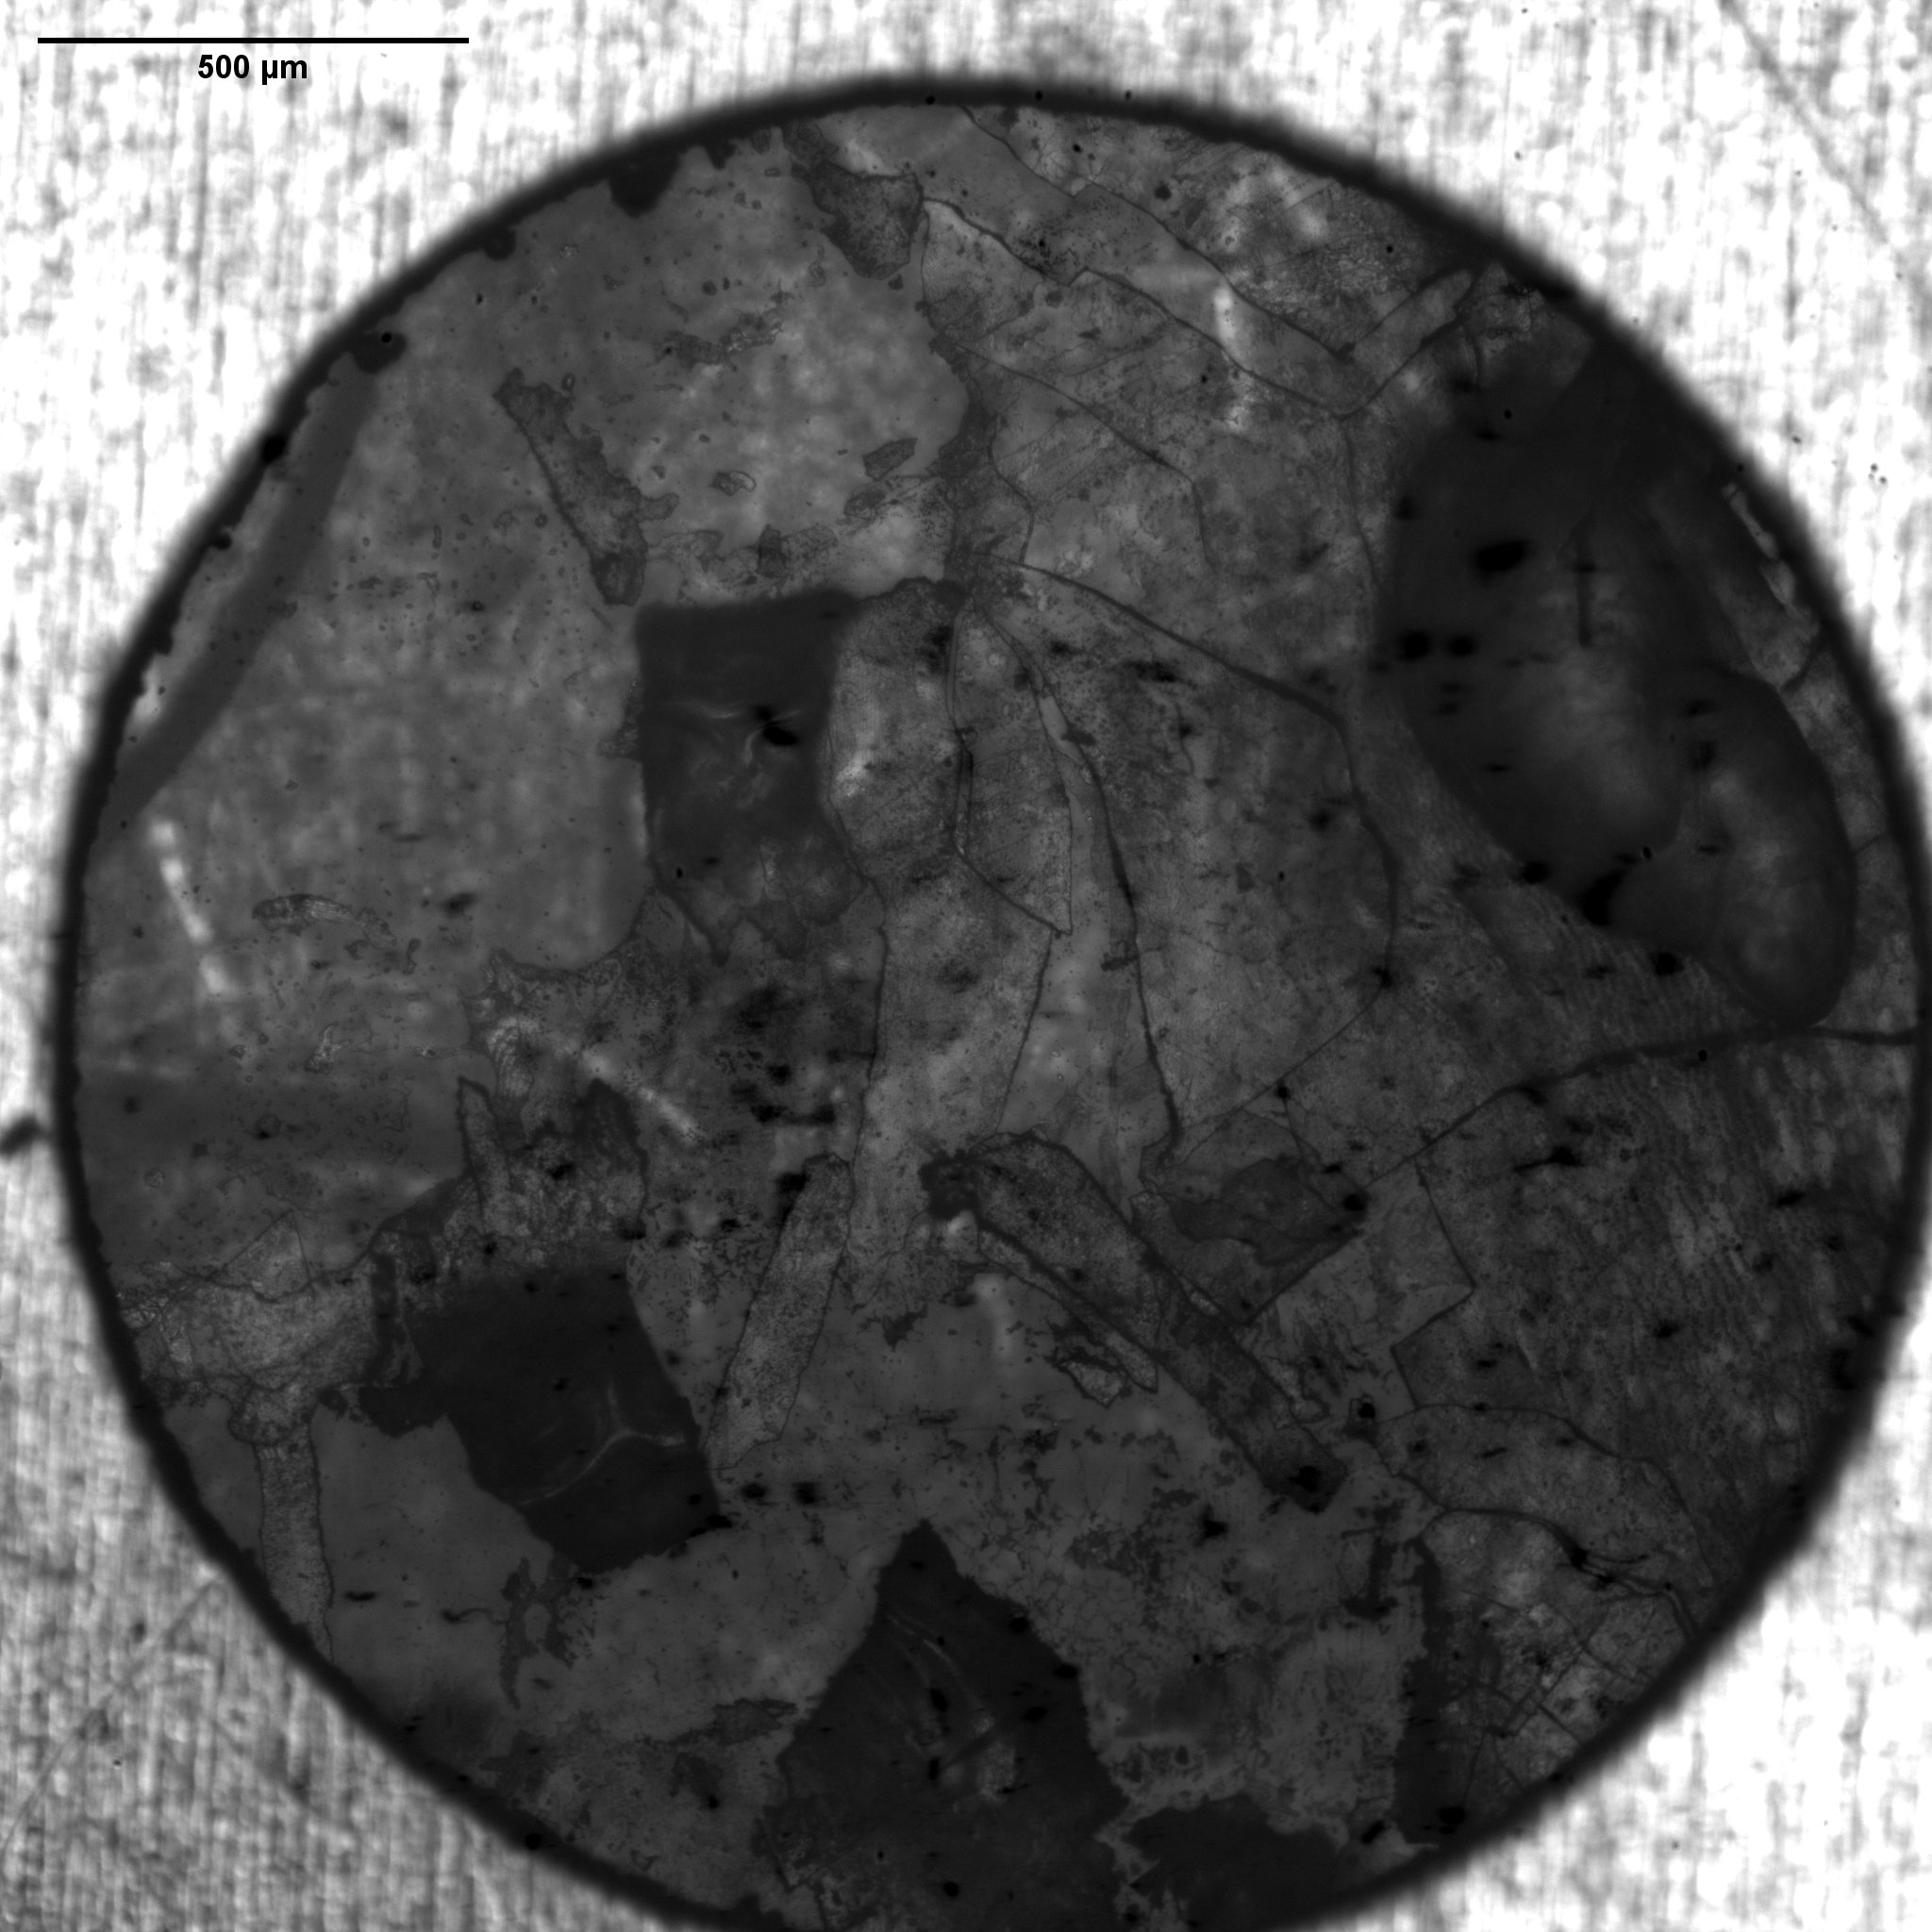
\includegraphics[width=7cm]{Hand freezed Lipid Broken Echtlicht.ome}
		\caption{Sample with a broken ice layer in true light \newline}
	\end{subfigure}
	\begin{subfigure}[]{0.45\textwidth}
		\centering
		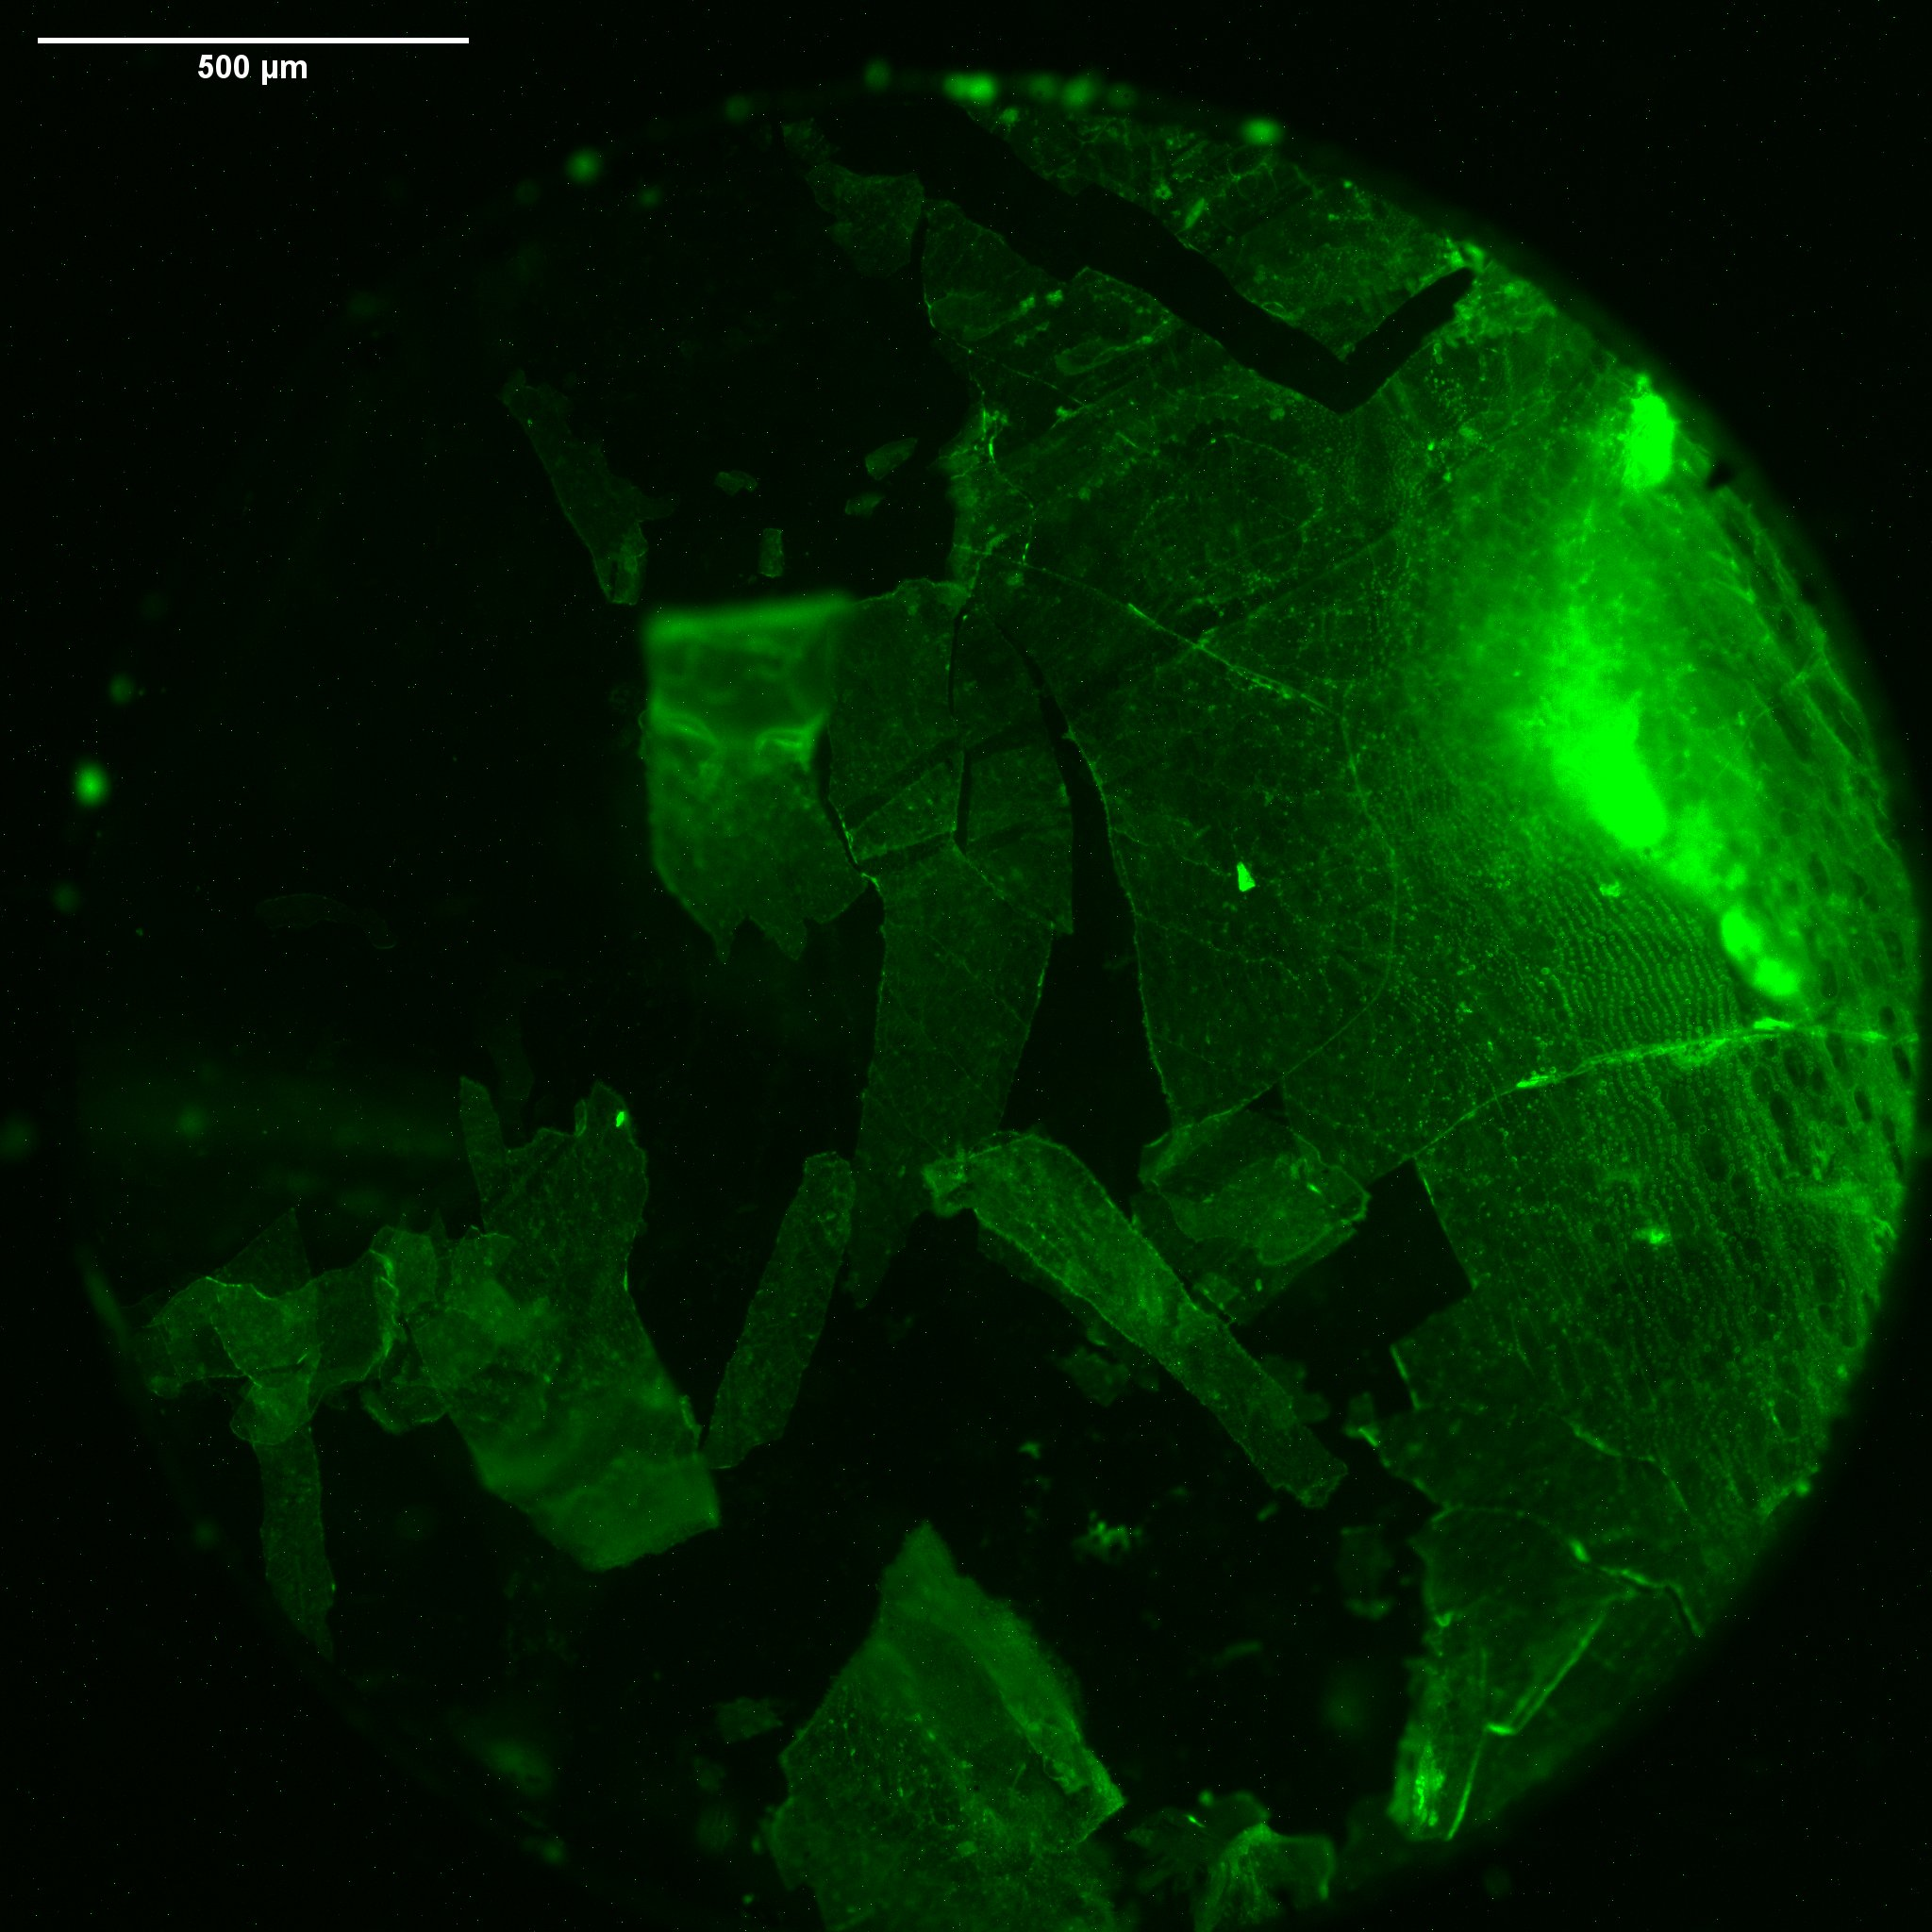
\includegraphics[width=7cm]{Hand freezed Lipid Broken Fluorescence.ome}
		\caption{Sample with a broken ice layer with fluorescence filter}
	\end{subfigure}
	\begin{subfigure}[]{0.45\textwidth}
		\centering
		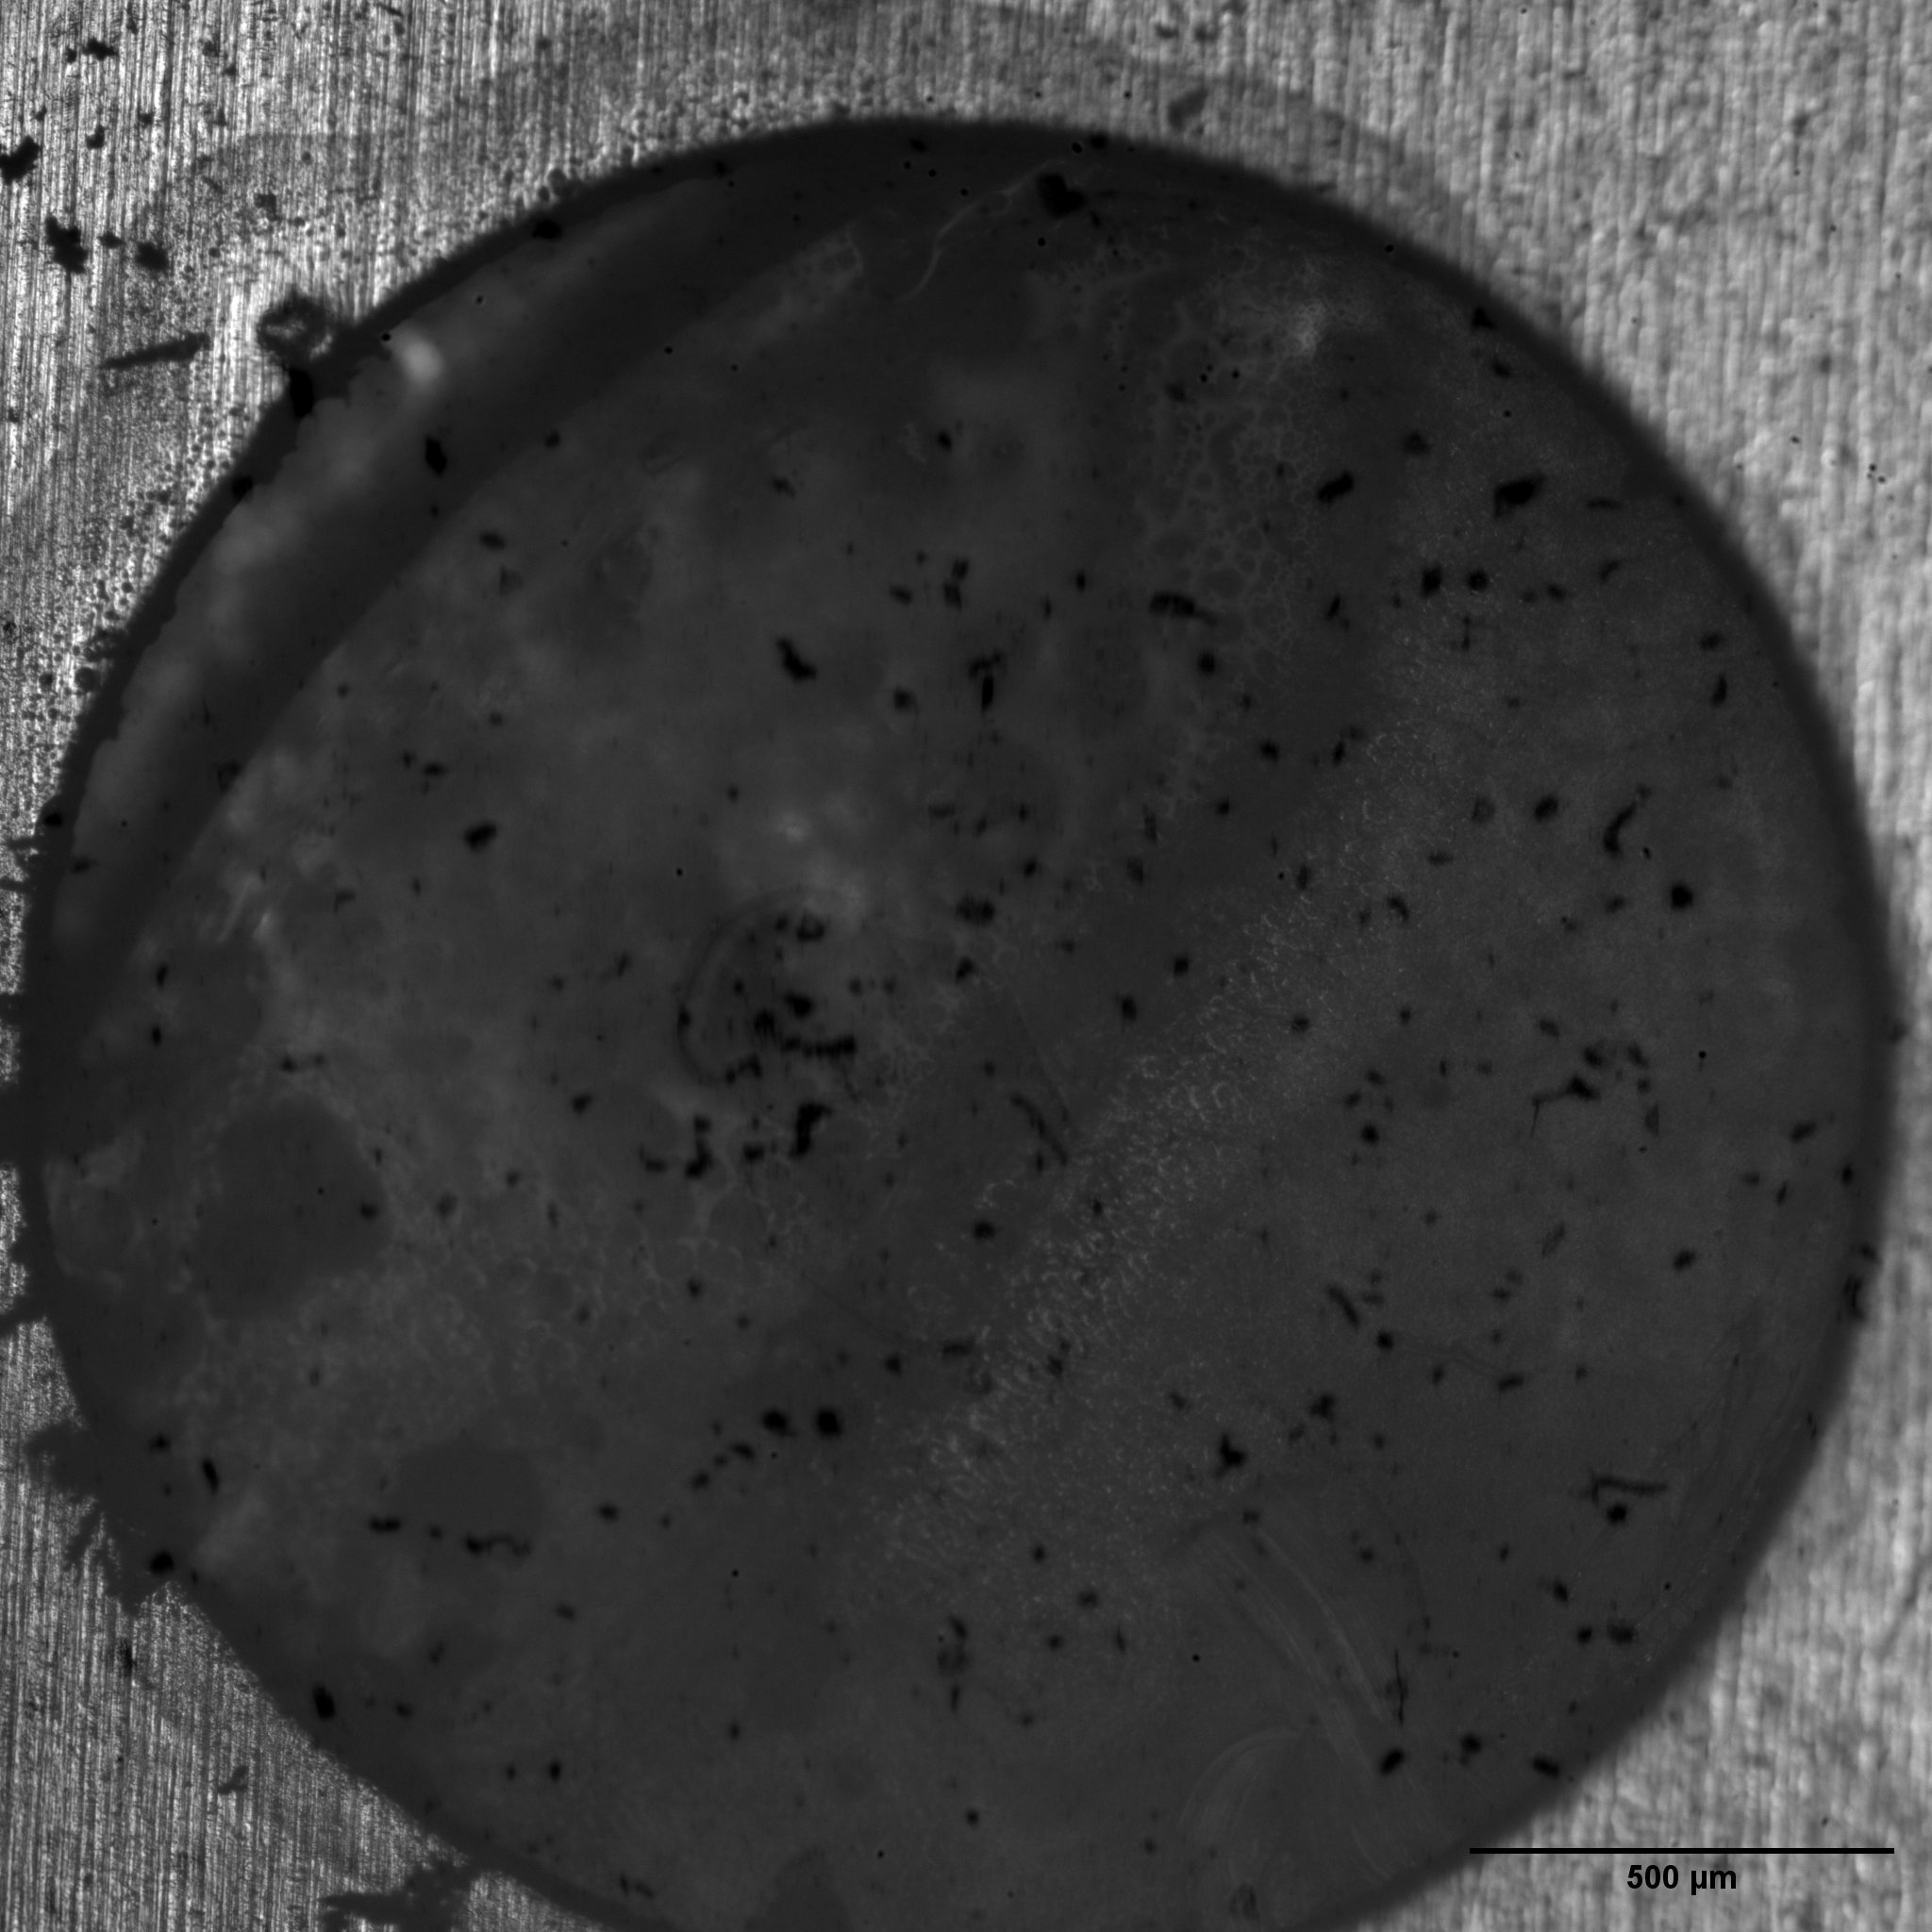
\includegraphics[width=7cm]{Hand freezed Lipid Continuous Echtlicht.ome}
		\caption{Sample with continuous ice layer in true light \newline}
	\end{subfigure}
	\begin{subfigure}[]{0.45\textwidth}
		\centering
		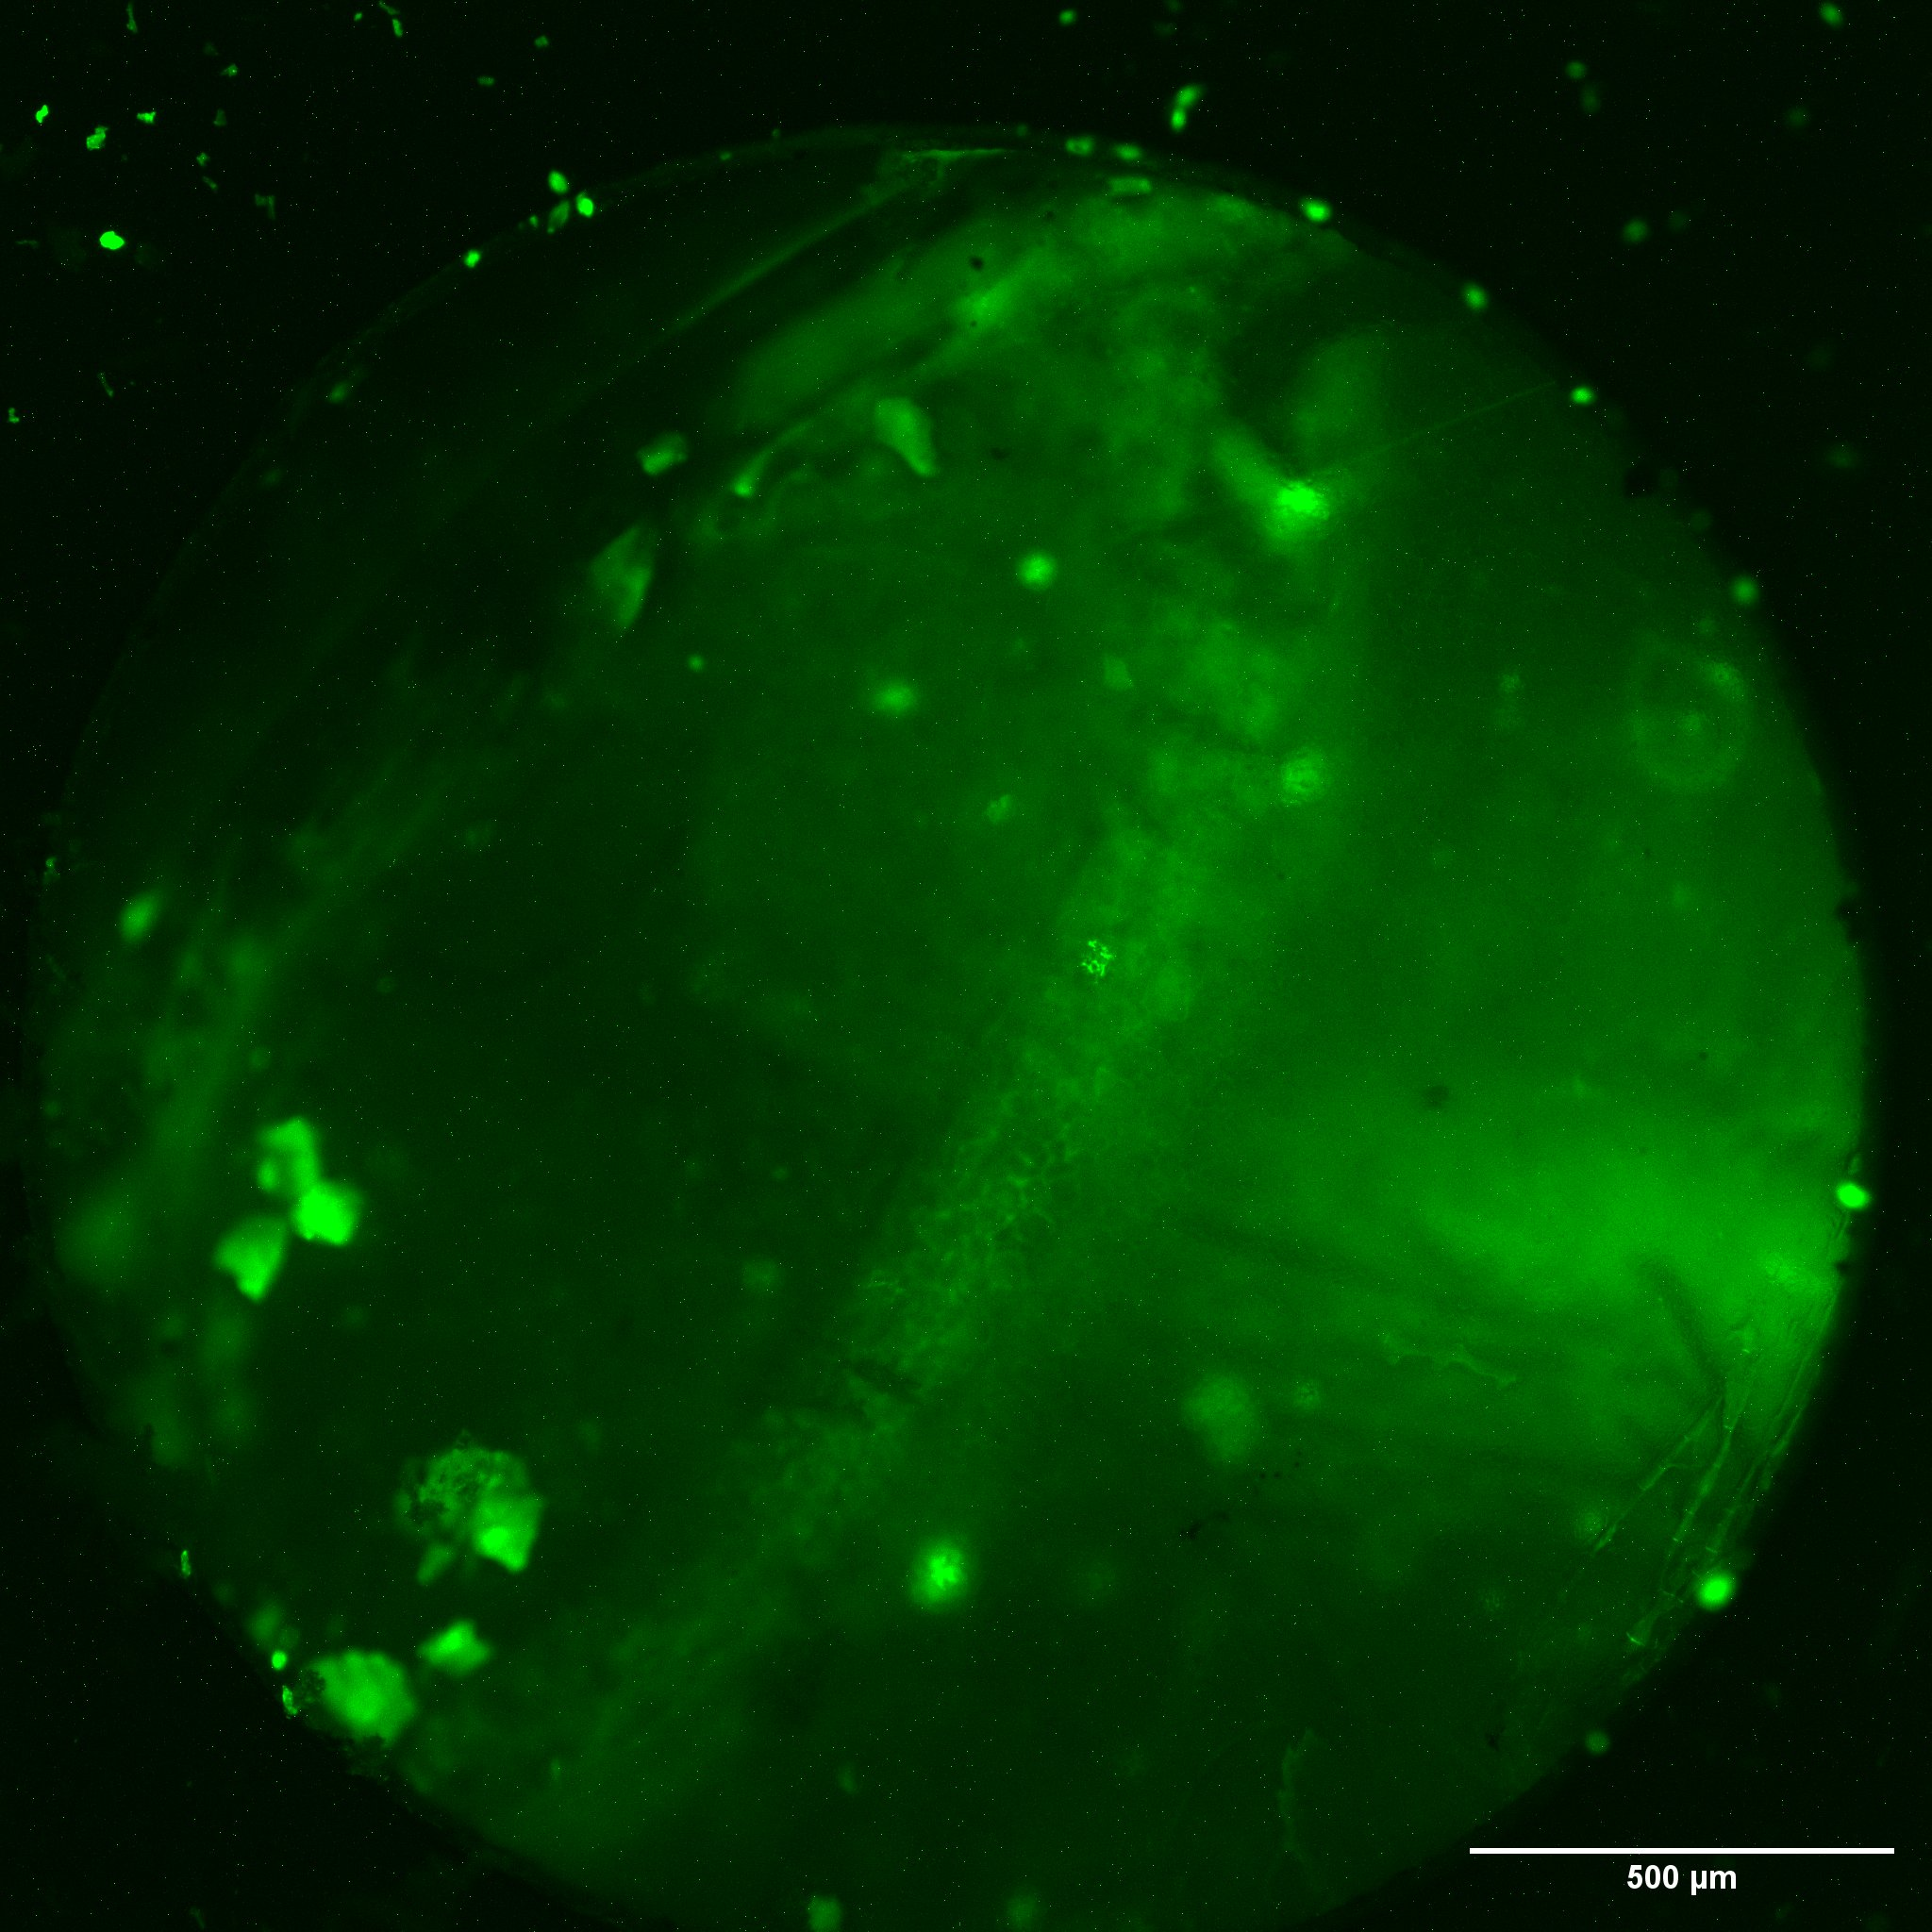
\includegraphics[width=7cm]{Hand freezed Lipid Continuous Fluorescence.ome}
		\caption{Sample with continuous ice layer with fluorescence filter}
	\end{subfigure}
	\caption{Two different examples for hand freezed ice layers on samples. }
	\label{fig:VglHandFreeze}
\end{figure}

\begin{figure}[hbt!]
	\centering
	\begin{subfigure}[]{0.45\textwidth}
		\centering
		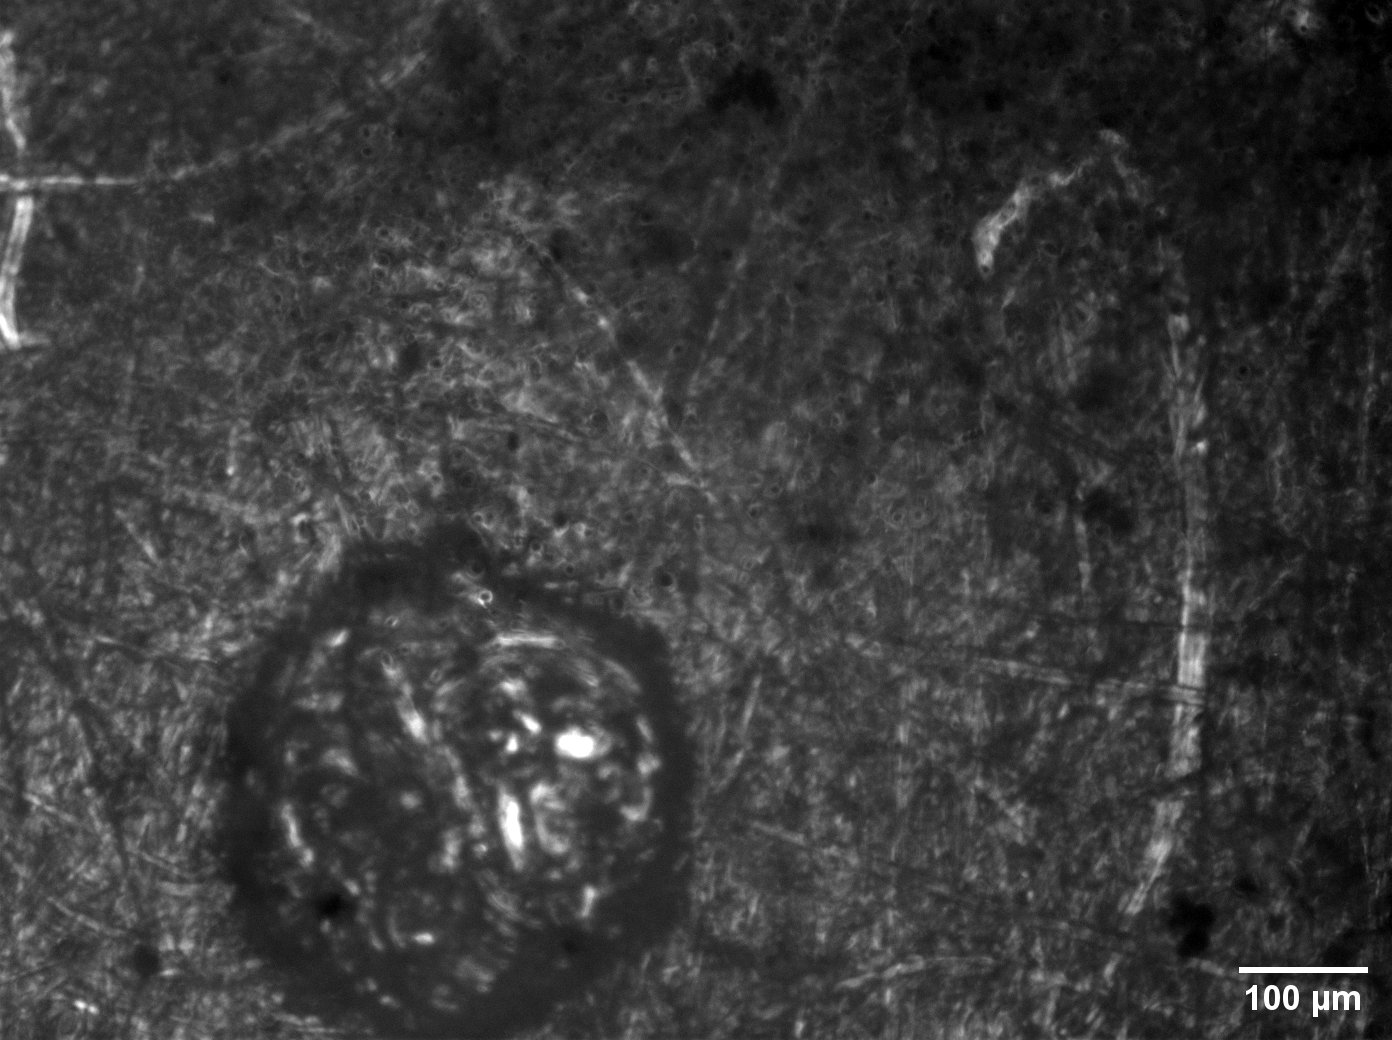
\includegraphics[width=7cm]{Thin Layer Plungefreezer Echtlicht.ome}
		\caption{Sample with thin continuous ice layer in true light \newline}
	\end{subfigure}
	\begin{subfigure}[]{0.45\textwidth}
		\centering
		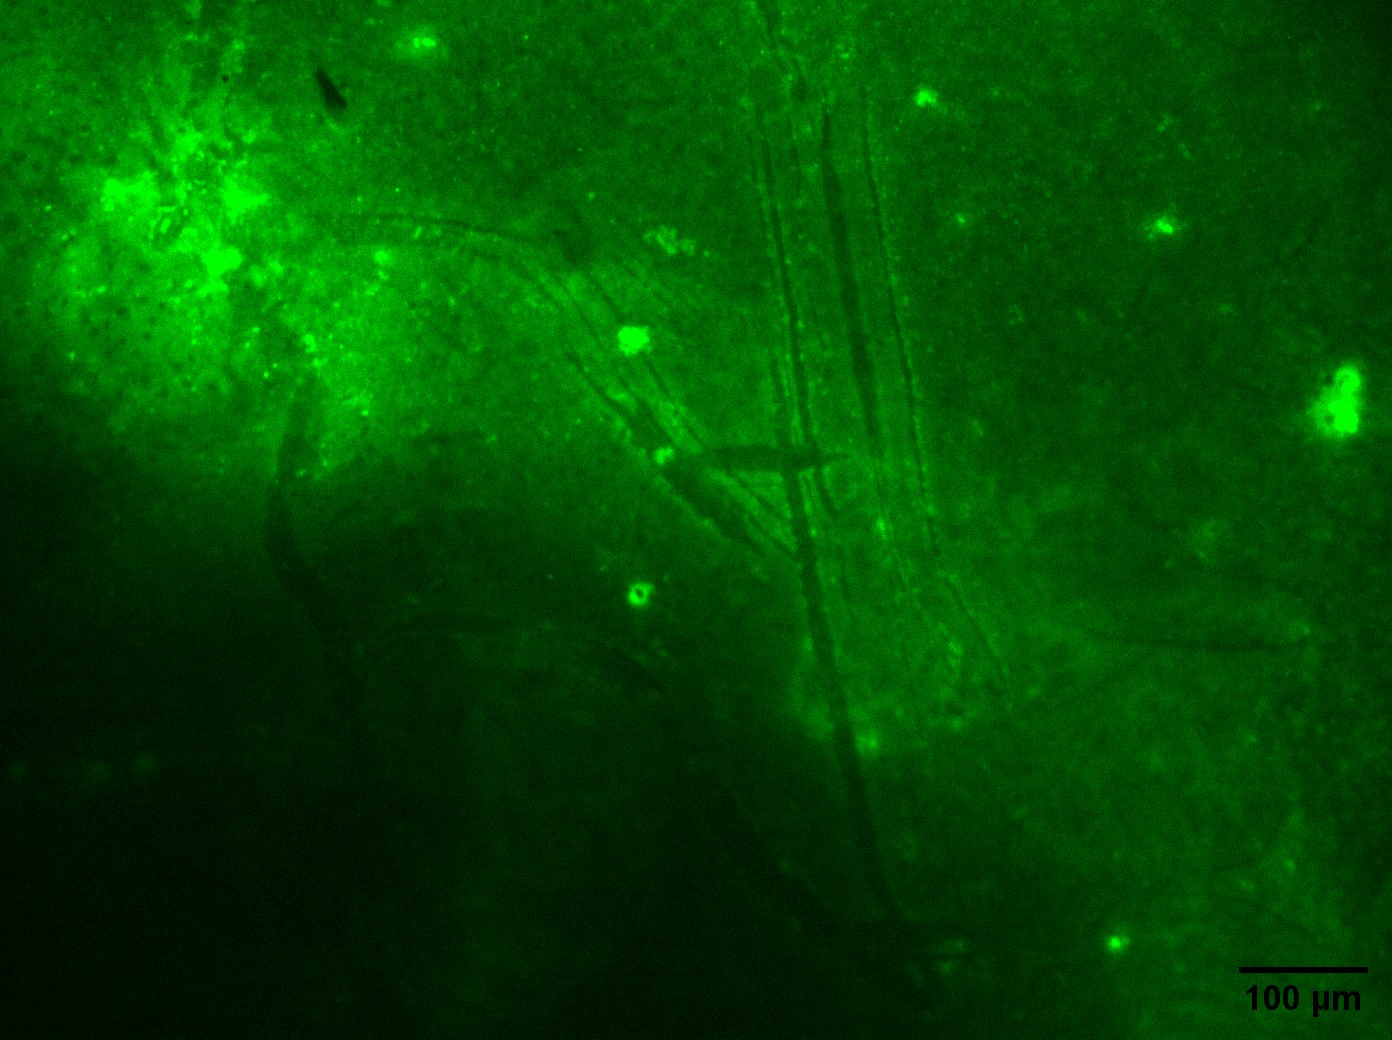
\includegraphics[width=7cm]{Thin Layer Plungefreezer Fluorescence.ome}
		\caption{Sample with thin continuous ice layer with fluorescence filter}
	\end{subfigure}
	\begin{subfigure}[]{0.45\textwidth}
		\centering
		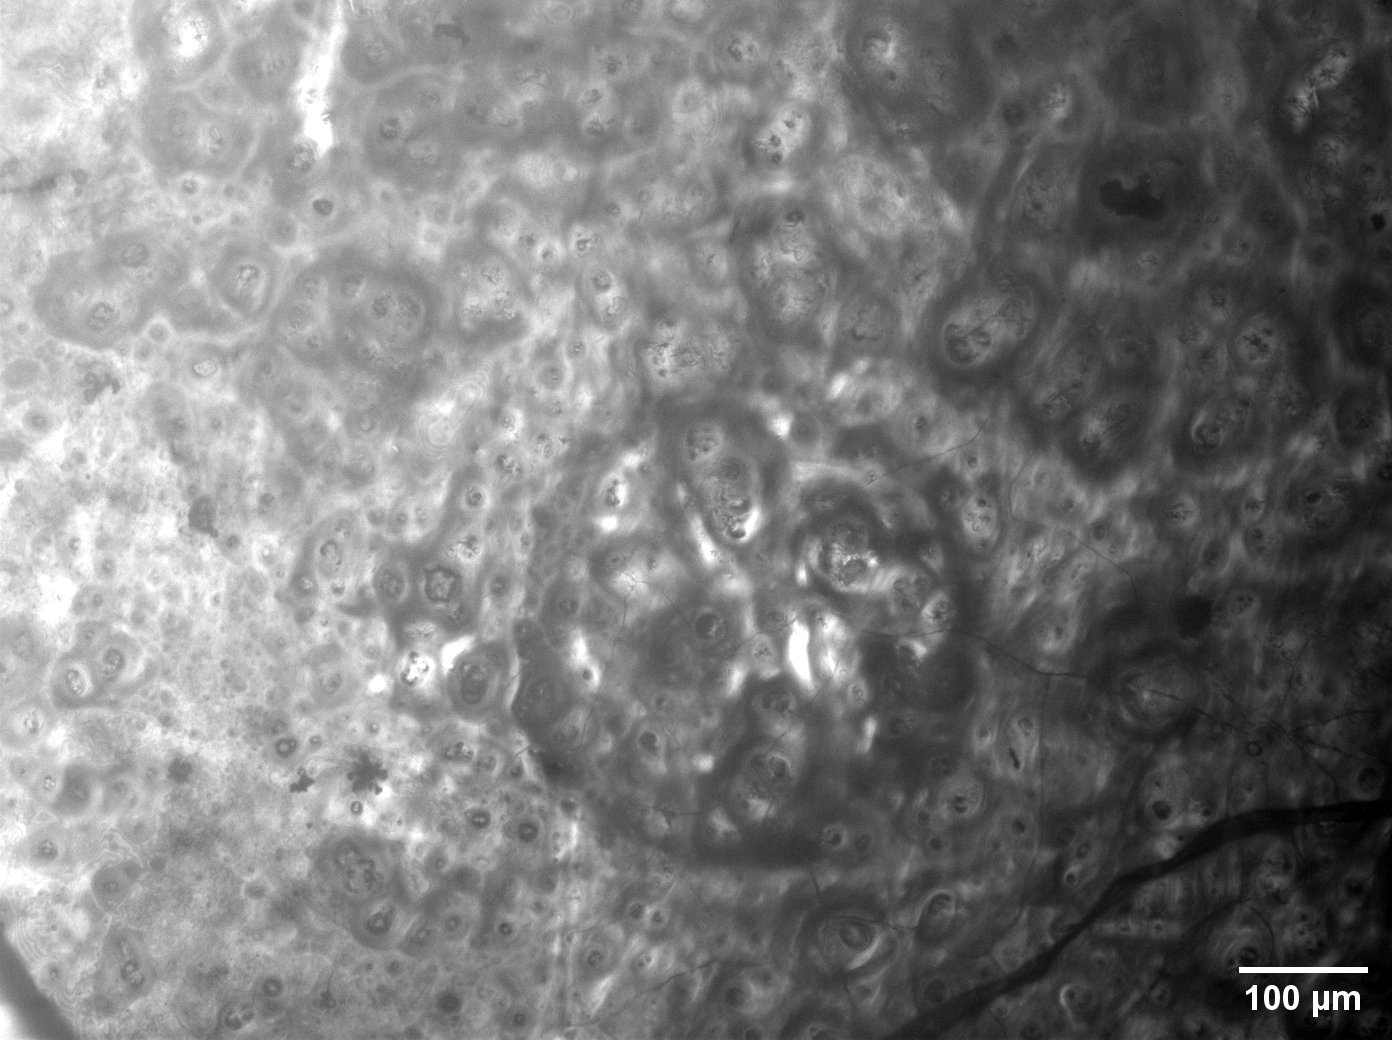
\includegraphics[width=7cm]{Thick Layer Plungefreezer Echtlicht.ome}
		\caption{Sample with thick continuous ice layer in true light with air bubbles}
	\end{subfigure}
	\begin{subfigure}[]{0.45\textwidth}
		\centering
		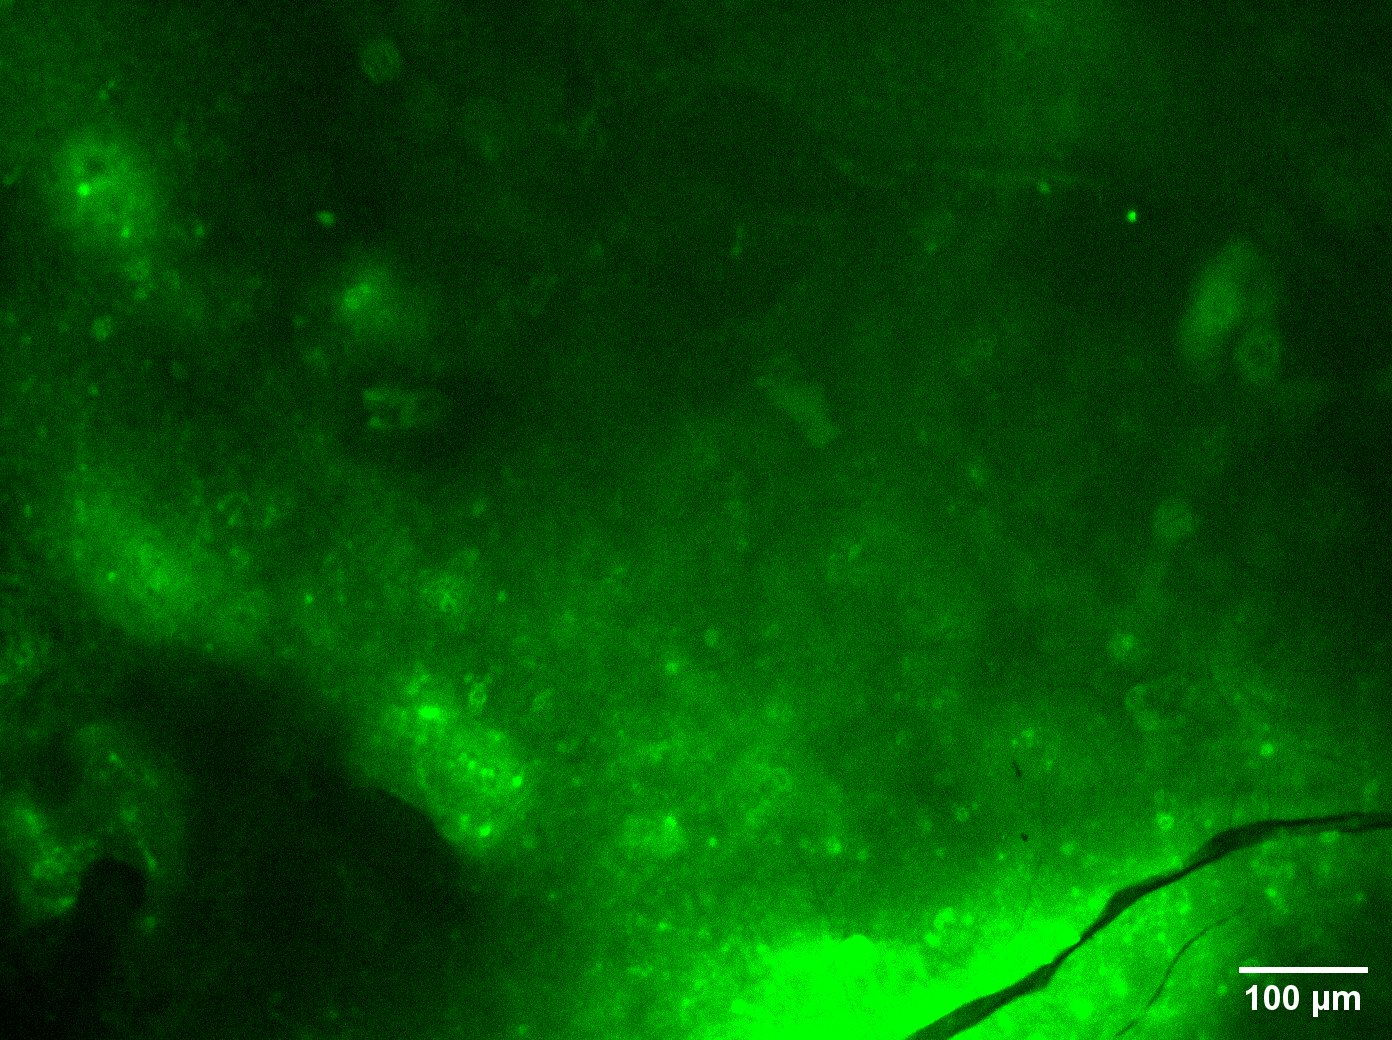
\includegraphics[width=7cm]{Thick Layer Plungefreezer Fluorescence.ome}
		\caption{Sample with thick continuous ice layer with fluorescence filter with air bubbles}
	\end{subfigure}
	\caption{Two different examples for hand freezed ice layers on samples. }
	\label{fig:VglMachineFreeze}
\end{figure}

To further compare plunge-freezed samples, 4 of each hand freezed and plunge freezed samples are compared regarding detachability. The "finger" is attached with HFE onto the sample. With movement up on the Z axis, the "finger" is inducing tensile force to the ice layer as an attempt to detach an ice piece.

The results are categorized in 4 categories: Not successful pulls don't have visible changes of the flourescent ice layer, Partially successes are visible breaks or clear movement of ice parts on the ice layer, Successful liftoff is a missing piece and a visible piece on the finger, which could be used for future steps. In the results, there is no difference between Hand freezed and plunge-freezed samples regarding detachability. Therefore Ice thickness is not a factor which makes detaching ice easier. As both methods don't show success in detaching ice pieces, it could still be a relevant factor but not a thing which should make a certain solution magically work xD

\begin{table}
	\centering
	\begin{tabular}{|c|c|c|}
		\hline
		Category & Hand-freezed & Plunge-freezed \\
		\hline
		\hline
		count executed tries & 4 & 4\\
		\hline
		unsuccessful & 3 & 3\\
		\hline
		breaks/movement of ice & 1 & 1\\
		\hline
		piece lifted with finger & 0 & 0\\
		\hline		
	\end{tabular}
	\caption{Comparison of detachability between hand-freezed and plunge-freezed samples}
\end{table}

\FloatBarrier

\subsection{other observed error sources??}

During experiments, other error sources are found. 

Zu viel abstand zu oberfläche

Integrität oberfläche

Finger kühlt zu langsam ab.

Wrong positioning, forming of ice

The formation of Ice inside the bath is largely inhibited through the Nitrogen Gas inlets. The nitrogen is forming a barrier to the atmosphere which contains humidity that turns into ice at cold temperatures. However, through turbulence and the finger, some ice can form inside the bath. 

In some experiments, high buildup of additional ice is observed on the sample. The additional ice is looser, reducing the possible grip onto the desired ice layer. The formation is traced back to a leakage in the finger. The tolerances between 3D printed part and metal bar should be able to seal the gap airtight. But trough changing out parts, the tolerances are looser, allowing a weak cold nitrogen current right on the sample. There are two possibility where the humidity itself is coming from: The cold nitrogen gas itself could contain some humidity. Second through additional turbulence, more air is sucked through the barrier. The air is directed directly on the sample, causing more ice buildup. To avoid this, the gap is sealed tight with tooth silicone????


\section{PDMS}

To speed up the process of finding the right balance of PDMS Mixture ratio and plasma curing, experiments at room temperature done. For this, a pulling machine is used. First the sample is prepared. Then, the sample is clamped to the pulling machine. Then a plexiglass stamp is aligned on top of the sample. With UV glue, the stamp is glued to the PDMS layer on the sample. Before gluing, the Force and distance is set to zero on the pulling machine. After gluing, a couple minutes are waited so no further stress changes are ongoing from the gluing process. then the Machine is pulling on the sample with constant velocity. After detachment, the measurement is stopped. Afterwards, the stamp and the layer are analyzed under a microscope. The area is determined. With the maximum force and area, the maximum stress is calculated. Each experiment is repeated multiple times.

\subsection{experiments at room temperature}

In between experiments, small variations are made: two different stamps are used, one has an area of \SI{2}{\milli\meter} x \SI{3}{\milli\meter} and another stamp is \SI{3}{\milli\meter} x \SI{3}{\milli\meter}. Since the area is measured afterwards, this should not have a significant effect on the results. Also, in the beginning, while waiting of the stress changes to subside, the pulling machine was inactive. with this, the Force before pulling will be higher as zero. Before pulling, the machine is set back to zero. After pulling, there is an offset between the neutral value and the value before because of zeroing, so the offset needs to be corrected. To avoid this, the pulling machine is set to zero force while waiting instead. Then no offset correction is needed. The offset correction and new method increased the accuracy between pull tests.

To verify the setup, samples coated with 4:1 and 1:2 curing agent to base coat weight ratio and uncoated coverglass used as slides are compared. The results show 2:1 mixture ratio with $87.3\pm19.9\,\si{\kilo\pascal}$ is easier to detach than 1:4 mixture ratio with $429.1\pm5.1\,\si{\kilo\pascal}$ (Fig. \ref{fig:vgl4:1zu1:2zuGlas}). Also glass without PDMS takes up a lot more tensile stress with $1161.5\pm111.5\,\si{\kilo\pascal}$. sometimes the machine is able to break the glass. Under the microscope, it is not visible if the PDMS layer itself was lifted from the glass or not.

\begin{figure}[hbt!]
	\centering	
	%% Creator: Matplotlib, PGF backend
%%
%% To include the figure in your LaTeX document, write
%%   \input{<filename>.pgf}
%%
%% Make sure the required packages are loaded in your preamble
%%   \usepackage{pgf}
%%
%% Also ensure that all the required font packages are loaded; for instance,
%% the lmodern package is sometimes necessary when using math font.
%%   \usepackage{lmodern}
%%
%% Figures using additional raster images can only be included by \input if
%% they are in the same directory as the main LaTeX file. For loading figures
%% from other directories you can use the `import` package
%%   \usepackage{import}
%%
%% and then include the figures with
%%   \import{<path to file>}{<filename>.pgf}
%%
%% Matplotlib used the following preamble
%%   
%%   \makeatletter\@ifpackageloaded{underscore}{}{\usepackage[strings]{underscore}}\makeatother
%%
\begingroup%
\makeatletter%
\begin{pgfpicture}%
\pgfpathrectangle{\pgfpointorigin}{\pgfqpoint{6.400000in}{4.800000in}}%
\pgfusepath{use as bounding box, clip}%
\begin{pgfscope}%
\pgfsetbuttcap%
\pgfsetmiterjoin%
\definecolor{currentfill}{rgb}{1.000000,1.000000,1.000000}%
\pgfsetfillcolor{currentfill}%
\pgfsetlinewidth{0.000000pt}%
\definecolor{currentstroke}{rgb}{1.000000,1.000000,1.000000}%
\pgfsetstrokecolor{currentstroke}%
\pgfsetdash{}{0pt}%
\pgfpathmoveto{\pgfqpoint{0.000000in}{0.000000in}}%
\pgfpathlineto{\pgfqpoint{6.400000in}{0.000000in}}%
\pgfpathlineto{\pgfqpoint{6.400000in}{4.800000in}}%
\pgfpathlineto{\pgfqpoint{0.000000in}{4.800000in}}%
\pgfpathlineto{\pgfqpoint{0.000000in}{0.000000in}}%
\pgfpathclose%
\pgfusepath{fill}%
\end{pgfscope}%
\begin{pgfscope}%
\pgfsetbuttcap%
\pgfsetmiterjoin%
\definecolor{currentfill}{rgb}{1.000000,1.000000,1.000000}%
\pgfsetfillcolor{currentfill}%
\pgfsetlinewidth{0.000000pt}%
\definecolor{currentstroke}{rgb}{0.000000,0.000000,0.000000}%
\pgfsetstrokecolor{currentstroke}%
\pgfsetstrokeopacity{0.000000}%
\pgfsetdash{}{0pt}%
\pgfpathmoveto{\pgfqpoint{0.800000in}{0.528000in}}%
\pgfpathlineto{\pgfqpoint{5.760000in}{0.528000in}}%
\pgfpathlineto{\pgfqpoint{5.760000in}{4.224000in}}%
\pgfpathlineto{\pgfqpoint{0.800000in}{4.224000in}}%
\pgfpathlineto{\pgfqpoint{0.800000in}{0.528000in}}%
\pgfpathclose%
\pgfusepath{fill}%
\end{pgfscope}%
\begin{pgfscope}%
\pgfpathrectangle{\pgfqpoint{0.800000in}{0.528000in}}{\pgfqpoint{4.960000in}{3.696000in}}%
\pgfusepath{clip}%
\pgfsetrectcap%
\pgfsetroundjoin%
\pgfsetlinewidth{0.803000pt}%
\definecolor{currentstroke}{rgb}{0.690196,0.690196,0.690196}%
\pgfsetstrokecolor{currentstroke}%
\pgfsetdash{}{0pt}%
\pgfpathmoveto{\pgfqpoint{1.626667in}{0.528000in}}%
\pgfpathlineto{\pgfqpoint{1.626667in}{4.224000in}}%
\pgfusepath{stroke}%
\end{pgfscope}%
\begin{pgfscope}%
\pgfsetbuttcap%
\pgfsetroundjoin%
\definecolor{currentfill}{rgb}{0.000000,0.000000,0.000000}%
\pgfsetfillcolor{currentfill}%
\pgfsetlinewidth{0.803000pt}%
\definecolor{currentstroke}{rgb}{0.000000,0.000000,0.000000}%
\pgfsetstrokecolor{currentstroke}%
\pgfsetdash{}{0pt}%
\pgfsys@defobject{currentmarker}{\pgfqpoint{0.000000in}{-0.048611in}}{\pgfqpoint{0.000000in}{0.000000in}}{%
\pgfpathmoveto{\pgfqpoint{0.000000in}{0.000000in}}%
\pgfpathlineto{\pgfqpoint{0.000000in}{-0.048611in}}%
\pgfusepath{stroke,fill}%
}%
\begin{pgfscope}%
\pgfsys@transformshift{1.626667in}{0.528000in}%
\pgfsys@useobject{currentmarker}{}%
\end{pgfscope}%
\end{pgfscope}%
\begin{pgfscope}%
\definecolor{textcolor}{rgb}{0.000000,0.000000,0.000000}%
\pgfsetstrokecolor{textcolor}%
\pgfsetfillcolor{textcolor}%
\pgftext[x=1.626667in,y=0.430778in,,top]{\color{textcolor}\rmfamily\fontsize{9.000000}{10.800000}\selectfont 1:2}%
\end{pgfscope}%
\begin{pgfscope}%
\pgfpathrectangle{\pgfqpoint{0.800000in}{0.528000in}}{\pgfqpoint{4.960000in}{3.696000in}}%
\pgfusepath{clip}%
\pgfsetrectcap%
\pgfsetroundjoin%
\pgfsetlinewidth{0.803000pt}%
\definecolor{currentstroke}{rgb}{0.690196,0.690196,0.690196}%
\pgfsetstrokecolor{currentstroke}%
\pgfsetdash{}{0pt}%
\pgfpathmoveto{\pgfqpoint{3.280000in}{0.528000in}}%
\pgfpathlineto{\pgfqpoint{3.280000in}{4.224000in}}%
\pgfusepath{stroke}%
\end{pgfscope}%
\begin{pgfscope}%
\pgfsetbuttcap%
\pgfsetroundjoin%
\definecolor{currentfill}{rgb}{0.000000,0.000000,0.000000}%
\pgfsetfillcolor{currentfill}%
\pgfsetlinewidth{0.803000pt}%
\definecolor{currentstroke}{rgb}{0.000000,0.000000,0.000000}%
\pgfsetstrokecolor{currentstroke}%
\pgfsetdash{}{0pt}%
\pgfsys@defobject{currentmarker}{\pgfqpoint{0.000000in}{-0.048611in}}{\pgfqpoint{0.000000in}{0.000000in}}{%
\pgfpathmoveto{\pgfqpoint{0.000000in}{0.000000in}}%
\pgfpathlineto{\pgfqpoint{0.000000in}{-0.048611in}}%
\pgfusepath{stroke,fill}%
}%
\begin{pgfscope}%
\pgfsys@transformshift{3.280000in}{0.528000in}%
\pgfsys@useobject{currentmarker}{}%
\end{pgfscope}%
\end{pgfscope}%
\begin{pgfscope}%
\definecolor{textcolor}{rgb}{0.000000,0.000000,0.000000}%
\pgfsetstrokecolor{textcolor}%
\pgfsetfillcolor{textcolor}%
\pgftext[x=3.280000in,y=0.430778in,,top]{\color{textcolor}\rmfamily\fontsize{9.000000}{10.800000}\selectfont 4:1}%
\end{pgfscope}%
\begin{pgfscope}%
\pgfpathrectangle{\pgfqpoint{0.800000in}{0.528000in}}{\pgfqpoint{4.960000in}{3.696000in}}%
\pgfusepath{clip}%
\pgfsetrectcap%
\pgfsetroundjoin%
\pgfsetlinewidth{0.803000pt}%
\definecolor{currentstroke}{rgb}{0.690196,0.690196,0.690196}%
\pgfsetstrokecolor{currentstroke}%
\pgfsetdash{}{0pt}%
\pgfpathmoveto{\pgfqpoint{4.933333in}{0.528000in}}%
\pgfpathlineto{\pgfqpoint{4.933333in}{4.224000in}}%
\pgfusepath{stroke}%
\end{pgfscope}%
\begin{pgfscope}%
\pgfsetbuttcap%
\pgfsetroundjoin%
\definecolor{currentfill}{rgb}{0.000000,0.000000,0.000000}%
\pgfsetfillcolor{currentfill}%
\pgfsetlinewidth{0.803000pt}%
\definecolor{currentstroke}{rgb}{0.000000,0.000000,0.000000}%
\pgfsetstrokecolor{currentstroke}%
\pgfsetdash{}{0pt}%
\pgfsys@defobject{currentmarker}{\pgfqpoint{0.000000in}{-0.048611in}}{\pgfqpoint{0.000000in}{0.000000in}}{%
\pgfpathmoveto{\pgfqpoint{0.000000in}{0.000000in}}%
\pgfpathlineto{\pgfqpoint{0.000000in}{-0.048611in}}%
\pgfusepath{stroke,fill}%
}%
\begin{pgfscope}%
\pgfsys@transformshift{4.933333in}{0.528000in}%
\pgfsys@useobject{currentmarker}{}%
\end{pgfscope}%
\end{pgfscope}%
\begin{pgfscope}%
\definecolor{textcolor}{rgb}{0.000000,0.000000,0.000000}%
\pgfsetstrokecolor{textcolor}%
\pgfsetfillcolor{textcolor}%
\pgftext[x=4.933333in,y=0.430778in,,top]{\color{textcolor}\rmfamily\fontsize{9.000000}{10.800000}\selectfont Glass without PDMS}%
\end{pgfscope}%
\begin{pgfscope}%
\pgfpathrectangle{\pgfqpoint{0.800000in}{0.528000in}}{\pgfqpoint{4.960000in}{3.696000in}}%
\pgfusepath{clip}%
\pgfsetrectcap%
\pgfsetroundjoin%
\pgfsetlinewidth{0.803000pt}%
\definecolor{currentstroke}{rgb}{0.690196,0.690196,0.690196}%
\pgfsetstrokecolor{currentstroke}%
\pgfsetdash{}{0pt}%
\pgfpathmoveto{\pgfqpoint{0.800000in}{1.065463in}}%
\pgfpathlineto{\pgfqpoint{5.760000in}{1.065463in}}%
\pgfusepath{stroke}%
\end{pgfscope}%
\begin{pgfscope}%
\pgfsetbuttcap%
\pgfsetroundjoin%
\definecolor{currentfill}{rgb}{0.000000,0.000000,0.000000}%
\pgfsetfillcolor{currentfill}%
\pgfsetlinewidth{0.803000pt}%
\definecolor{currentstroke}{rgb}{0.000000,0.000000,0.000000}%
\pgfsetstrokecolor{currentstroke}%
\pgfsetdash{}{0pt}%
\pgfsys@defobject{currentmarker}{\pgfqpoint{-0.048611in}{0.000000in}}{\pgfqpoint{-0.000000in}{0.000000in}}{%
\pgfpathmoveto{\pgfqpoint{-0.000000in}{0.000000in}}%
\pgfpathlineto{\pgfqpoint{-0.048611in}{0.000000in}}%
\pgfusepath{stroke,fill}%
}%
\begin{pgfscope}%
\pgfsys@transformshift{0.800000in}{1.065463in}%
\pgfsys@useobject{currentmarker}{}%
\end{pgfscope}%
\end{pgfscope}%
\begin{pgfscope}%
\definecolor{textcolor}{rgb}{0.000000,0.000000,0.000000}%
\pgfsetstrokecolor{textcolor}%
\pgfsetfillcolor{textcolor}%
\pgftext[x=0.494444in, y=1.017237in, left, base]{\color{textcolor}\rmfamily\fontsize{10.000000}{12.000000}\selectfont \(\displaystyle {200}\)}%
\end{pgfscope}%
\begin{pgfscope}%
\pgfpathrectangle{\pgfqpoint{0.800000in}{0.528000in}}{\pgfqpoint{4.960000in}{3.696000in}}%
\pgfusepath{clip}%
\pgfsetrectcap%
\pgfsetroundjoin%
\pgfsetlinewidth{0.803000pt}%
\definecolor{currentstroke}{rgb}{0.690196,0.690196,0.690196}%
\pgfsetstrokecolor{currentstroke}%
\pgfsetdash{}{0pt}%
\pgfpathmoveto{\pgfqpoint{0.800000in}{1.622908in}}%
\pgfpathlineto{\pgfqpoint{5.760000in}{1.622908in}}%
\pgfusepath{stroke}%
\end{pgfscope}%
\begin{pgfscope}%
\pgfsetbuttcap%
\pgfsetroundjoin%
\definecolor{currentfill}{rgb}{0.000000,0.000000,0.000000}%
\pgfsetfillcolor{currentfill}%
\pgfsetlinewidth{0.803000pt}%
\definecolor{currentstroke}{rgb}{0.000000,0.000000,0.000000}%
\pgfsetstrokecolor{currentstroke}%
\pgfsetdash{}{0pt}%
\pgfsys@defobject{currentmarker}{\pgfqpoint{-0.048611in}{0.000000in}}{\pgfqpoint{-0.000000in}{0.000000in}}{%
\pgfpathmoveto{\pgfqpoint{-0.000000in}{0.000000in}}%
\pgfpathlineto{\pgfqpoint{-0.048611in}{0.000000in}}%
\pgfusepath{stroke,fill}%
}%
\begin{pgfscope}%
\pgfsys@transformshift{0.800000in}{1.622908in}%
\pgfsys@useobject{currentmarker}{}%
\end{pgfscope}%
\end{pgfscope}%
\begin{pgfscope}%
\definecolor{textcolor}{rgb}{0.000000,0.000000,0.000000}%
\pgfsetstrokecolor{textcolor}%
\pgfsetfillcolor{textcolor}%
\pgftext[x=0.494444in, y=1.574683in, left, base]{\color{textcolor}\rmfamily\fontsize{10.000000}{12.000000}\selectfont \(\displaystyle {400}\)}%
\end{pgfscope}%
\begin{pgfscope}%
\pgfpathrectangle{\pgfqpoint{0.800000in}{0.528000in}}{\pgfqpoint{4.960000in}{3.696000in}}%
\pgfusepath{clip}%
\pgfsetrectcap%
\pgfsetroundjoin%
\pgfsetlinewidth{0.803000pt}%
\definecolor{currentstroke}{rgb}{0.690196,0.690196,0.690196}%
\pgfsetstrokecolor{currentstroke}%
\pgfsetdash{}{0pt}%
\pgfpathmoveto{\pgfqpoint{0.800000in}{2.180354in}}%
\pgfpathlineto{\pgfqpoint{5.760000in}{2.180354in}}%
\pgfusepath{stroke}%
\end{pgfscope}%
\begin{pgfscope}%
\pgfsetbuttcap%
\pgfsetroundjoin%
\definecolor{currentfill}{rgb}{0.000000,0.000000,0.000000}%
\pgfsetfillcolor{currentfill}%
\pgfsetlinewidth{0.803000pt}%
\definecolor{currentstroke}{rgb}{0.000000,0.000000,0.000000}%
\pgfsetstrokecolor{currentstroke}%
\pgfsetdash{}{0pt}%
\pgfsys@defobject{currentmarker}{\pgfqpoint{-0.048611in}{0.000000in}}{\pgfqpoint{-0.000000in}{0.000000in}}{%
\pgfpathmoveto{\pgfqpoint{-0.000000in}{0.000000in}}%
\pgfpathlineto{\pgfqpoint{-0.048611in}{0.000000in}}%
\pgfusepath{stroke,fill}%
}%
\begin{pgfscope}%
\pgfsys@transformshift{0.800000in}{2.180354in}%
\pgfsys@useobject{currentmarker}{}%
\end{pgfscope}%
\end{pgfscope}%
\begin{pgfscope}%
\definecolor{textcolor}{rgb}{0.000000,0.000000,0.000000}%
\pgfsetstrokecolor{textcolor}%
\pgfsetfillcolor{textcolor}%
\pgftext[x=0.494444in, y=2.132128in, left, base]{\color{textcolor}\rmfamily\fontsize{10.000000}{12.000000}\selectfont \(\displaystyle {600}\)}%
\end{pgfscope}%
\begin{pgfscope}%
\pgfpathrectangle{\pgfqpoint{0.800000in}{0.528000in}}{\pgfqpoint{4.960000in}{3.696000in}}%
\pgfusepath{clip}%
\pgfsetrectcap%
\pgfsetroundjoin%
\pgfsetlinewidth{0.803000pt}%
\definecolor{currentstroke}{rgb}{0.690196,0.690196,0.690196}%
\pgfsetstrokecolor{currentstroke}%
\pgfsetdash{}{0pt}%
\pgfpathmoveto{\pgfqpoint{0.800000in}{2.737799in}}%
\pgfpathlineto{\pgfqpoint{5.760000in}{2.737799in}}%
\pgfusepath{stroke}%
\end{pgfscope}%
\begin{pgfscope}%
\pgfsetbuttcap%
\pgfsetroundjoin%
\definecolor{currentfill}{rgb}{0.000000,0.000000,0.000000}%
\pgfsetfillcolor{currentfill}%
\pgfsetlinewidth{0.803000pt}%
\definecolor{currentstroke}{rgb}{0.000000,0.000000,0.000000}%
\pgfsetstrokecolor{currentstroke}%
\pgfsetdash{}{0pt}%
\pgfsys@defobject{currentmarker}{\pgfqpoint{-0.048611in}{0.000000in}}{\pgfqpoint{-0.000000in}{0.000000in}}{%
\pgfpathmoveto{\pgfqpoint{-0.000000in}{0.000000in}}%
\pgfpathlineto{\pgfqpoint{-0.048611in}{0.000000in}}%
\pgfusepath{stroke,fill}%
}%
\begin{pgfscope}%
\pgfsys@transformshift{0.800000in}{2.737799in}%
\pgfsys@useobject{currentmarker}{}%
\end{pgfscope}%
\end{pgfscope}%
\begin{pgfscope}%
\definecolor{textcolor}{rgb}{0.000000,0.000000,0.000000}%
\pgfsetstrokecolor{textcolor}%
\pgfsetfillcolor{textcolor}%
\pgftext[x=0.494444in, y=2.689574in, left, base]{\color{textcolor}\rmfamily\fontsize{10.000000}{12.000000}\selectfont \(\displaystyle {800}\)}%
\end{pgfscope}%
\begin{pgfscope}%
\pgfpathrectangle{\pgfqpoint{0.800000in}{0.528000in}}{\pgfqpoint{4.960000in}{3.696000in}}%
\pgfusepath{clip}%
\pgfsetrectcap%
\pgfsetroundjoin%
\pgfsetlinewidth{0.803000pt}%
\definecolor{currentstroke}{rgb}{0.690196,0.690196,0.690196}%
\pgfsetstrokecolor{currentstroke}%
\pgfsetdash{}{0pt}%
\pgfpathmoveto{\pgfqpoint{0.800000in}{3.295245in}}%
\pgfpathlineto{\pgfqpoint{5.760000in}{3.295245in}}%
\pgfusepath{stroke}%
\end{pgfscope}%
\begin{pgfscope}%
\pgfsetbuttcap%
\pgfsetroundjoin%
\definecolor{currentfill}{rgb}{0.000000,0.000000,0.000000}%
\pgfsetfillcolor{currentfill}%
\pgfsetlinewidth{0.803000pt}%
\definecolor{currentstroke}{rgb}{0.000000,0.000000,0.000000}%
\pgfsetstrokecolor{currentstroke}%
\pgfsetdash{}{0pt}%
\pgfsys@defobject{currentmarker}{\pgfqpoint{-0.048611in}{0.000000in}}{\pgfqpoint{-0.000000in}{0.000000in}}{%
\pgfpathmoveto{\pgfqpoint{-0.000000in}{0.000000in}}%
\pgfpathlineto{\pgfqpoint{-0.048611in}{0.000000in}}%
\pgfusepath{stroke,fill}%
}%
\begin{pgfscope}%
\pgfsys@transformshift{0.800000in}{3.295245in}%
\pgfsys@useobject{currentmarker}{}%
\end{pgfscope}%
\end{pgfscope}%
\begin{pgfscope}%
\definecolor{textcolor}{rgb}{0.000000,0.000000,0.000000}%
\pgfsetstrokecolor{textcolor}%
\pgfsetfillcolor{textcolor}%
\pgftext[x=0.424999in, y=3.247020in, left, base]{\color{textcolor}\rmfamily\fontsize{10.000000}{12.000000}\selectfont \(\displaystyle {1000}\)}%
\end{pgfscope}%
\begin{pgfscope}%
\pgfpathrectangle{\pgfqpoint{0.800000in}{0.528000in}}{\pgfqpoint{4.960000in}{3.696000in}}%
\pgfusepath{clip}%
\pgfsetrectcap%
\pgfsetroundjoin%
\pgfsetlinewidth{0.803000pt}%
\definecolor{currentstroke}{rgb}{0.690196,0.690196,0.690196}%
\pgfsetstrokecolor{currentstroke}%
\pgfsetdash{}{0pt}%
\pgfpathmoveto{\pgfqpoint{0.800000in}{3.852690in}}%
\pgfpathlineto{\pgfqpoint{5.760000in}{3.852690in}}%
\pgfusepath{stroke}%
\end{pgfscope}%
\begin{pgfscope}%
\pgfsetbuttcap%
\pgfsetroundjoin%
\definecolor{currentfill}{rgb}{0.000000,0.000000,0.000000}%
\pgfsetfillcolor{currentfill}%
\pgfsetlinewidth{0.803000pt}%
\definecolor{currentstroke}{rgb}{0.000000,0.000000,0.000000}%
\pgfsetstrokecolor{currentstroke}%
\pgfsetdash{}{0pt}%
\pgfsys@defobject{currentmarker}{\pgfqpoint{-0.048611in}{0.000000in}}{\pgfqpoint{-0.000000in}{0.000000in}}{%
\pgfpathmoveto{\pgfqpoint{-0.000000in}{0.000000in}}%
\pgfpathlineto{\pgfqpoint{-0.048611in}{0.000000in}}%
\pgfusepath{stroke,fill}%
}%
\begin{pgfscope}%
\pgfsys@transformshift{0.800000in}{3.852690in}%
\pgfsys@useobject{currentmarker}{}%
\end{pgfscope}%
\end{pgfscope}%
\begin{pgfscope}%
\definecolor{textcolor}{rgb}{0.000000,0.000000,0.000000}%
\pgfsetstrokecolor{textcolor}%
\pgfsetfillcolor{textcolor}%
\pgftext[x=0.424999in, y=3.804465in, left, base]{\color{textcolor}\rmfamily\fontsize{10.000000}{12.000000}\selectfont \(\displaystyle {1200}\)}%
\end{pgfscope}%
\begin{pgfscope}%
\definecolor{textcolor}{rgb}{0.000000,0.000000,0.000000}%
\pgfsetstrokecolor{textcolor}%
\pgfsetfillcolor{textcolor}%
\pgftext[x=0.369444in,y=2.376000in,,bottom,rotate=90.000000]{\color{textcolor}\rmfamily\fontsize{10.000000}{12.000000}\selectfont Tensile stress in kPA}%
\end{pgfscope}%
\begin{pgfscope}%
\pgfpathrectangle{\pgfqpoint{0.800000in}{0.528000in}}{\pgfqpoint{4.960000in}{3.696000in}}%
\pgfusepath{clip}%
\pgfsetbuttcap%
\pgfsetroundjoin%
\pgfsetlinewidth{1.505625pt}%
\definecolor{currentstroke}{rgb}{0.121569,0.466667,0.705882}%
\pgfsetstrokecolor{currentstroke}%
\pgfsetdash{}{0pt}%
\pgfpathmoveto{\pgfqpoint{1.626667in}{0.696000in}}%
\pgfpathlineto{\pgfqpoint{1.626667in}{0.807188in}}%
\pgfusepath{stroke}%
\end{pgfscope}%
\begin{pgfscope}%
\pgfpathrectangle{\pgfqpoint{0.800000in}{0.528000in}}{\pgfqpoint{4.960000in}{3.696000in}}%
\pgfusepath{clip}%
\pgfsetbuttcap%
\pgfsetroundjoin%
\pgfsetlinewidth{1.505625pt}%
\definecolor{currentstroke}{rgb}{0.121569,0.466667,0.705882}%
\pgfsetstrokecolor{currentstroke}%
\pgfsetdash{}{0pt}%
\pgfpathmoveto{\pgfqpoint{3.280000in}{1.690009in}}%
\pgfpathlineto{\pgfqpoint{3.280000in}{1.718231in}}%
\pgfusepath{stroke}%
\end{pgfscope}%
\begin{pgfscope}%
\pgfpathrectangle{\pgfqpoint{0.800000in}{0.528000in}}{\pgfqpoint{4.960000in}{3.696000in}}%
\pgfusepath{clip}%
\pgfsetbuttcap%
\pgfsetroundjoin%
\pgfsetlinewidth{1.505625pt}%
\definecolor{currentstroke}{rgb}{0.121569,0.466667,0.705882}%
\pgfsetstrokecolor{currentstroke}%
\pgfsetdash{}{0pt}%
\pgfpathmoveto{\pgfqpoint{4.933333in}{3.434536in}}%
\pgfpathlineto{\pgfqpoint{4.933333in}{4.056000in}}%
\pgfusepath{stroke}%
\end{pgfscope}%
\begin{pgfscope}%
\pgfpathrectangle{\pgfqpoint{0.800000in}{0.528000in}}{\pgfqpoint{4.960000in}{3.696000in}}%
\pgfusepath{clip}%
\pgfsetbuttcap%
\pgfsetroundjoin%
\definecolor{currentfill}{rgb}{0.121569,0.466667,0.705882}%
\pgfsetfillcolor{currentfill}%
\pgfsetlinewidth{1.003750pt}%
\definecolor{currentstroke}{rgb}{0.121569,0.466667,0.705882}%
\pgfsetstrokecolor{currentstroke}%
\pgfsetdash{}{0pt}%
\pgfsys@defobject{currentmarker}{\pgfqpoint{-0.111111in}{-0.000000in}}{\pgfqpoint{0.111111in}{0.000000in}}{%
\pgfpathmoveto{\pgfqpoint{0.111111in}{-0.000000in}}%
\pgfpathlineto{\pgfqpoint{-0.111111in}{0.000000in}}%
\pgfusepath{stroke,fill}%
}%
\begin{pgfscope}%
\pgfsys@transformshift{1.626667in}{0.696000in}%
\pgfsys@useobject{currentmarker}{}%
\end{pgfscope}%
\begin{pgfscope}%
\pgfsys@transformshift{3.280000in}{1.690009in}%
\pgfsys@useobject{currentmarker}{}%
\end{pgfscope}%
\begin{pgfscope}%
\pgfsys@transformshift{4.933333in}{3.434536in}%
\pgfsys@useobject{currentmarker}{}%
\end{pgfscope}%
\end{pgfscope}%
\begin{pgfscope}%
\pgfpathrectangle{\pgfqpoint{0.800000in}{0.528000in}}{\pgfqpoint{4.960000in}{3.696000in}}%
\pgfusepath{clip}%
\pgfsetbuttcap%
\pgfsetroundjoin%
\definecolor{currentfill}{rgb}{0.121569,0.466667,0.705882}%
\pgfsetfillcolor{currentfill}%
\pgfsetlinewidth{1.003750pt}%
\definecolor{currentstroke}{rgb}{0.121569,0.466667,0.705882}%
\pgfsetstrokecolor{currentstroke}%
\pgfsetdash{}{0pt}%
\pgfsys@defobject{currentmarker}{\pgfqpoint{-0.111111in}{-0.000000in}}{\pgfqpoint{0.111111in}{0.000000in}}{%
\pgfpathmoveto{\pgfqpoint{0.111111in}{-0.000000in}}%
\pgfpathlineto{\pgfqpoint{-0.111111in}{0.000000in}}%
\pgfusepath{stroke,fill}%
}%
\begin{pgfscope}%
\pgfsys@transformshift{1.626667in}{0.807188in}%
\pgfsys@useobject{currentmarker}{}%
\end{pgfscope}%
\begin{pgfscope}%
\pgfsys@transformshift{3.280000in}{1.718231in}%
\pgfsys@useobject{currentmarker}{}%
\end{pgfscope}%
\begin{pgfscope}%
\pgfsys@transformshift{4.933333in}{4.056000in}%
\pgfsys@useobject{currentmarker}{}%
\end{pgfscope}%
\end{pgfscope}%
\begin{pgfscope}%
\pgfpathrectangle{\pgfqpoint{0.800000in}{0.528000in}}{\pgfqpoint{4.960000in}{3.696000in}}%
\pgfusepath{clip}%
\pgfsetbuttcap%
\pgfsetroundjoin%
\definecolor{currentfill}{rgb}{0.121569,0.466667,0.705882}%
\pgfsetfillcolor{currentfill}%
\pgfsetlinewidth{1.003750pt}%
\definecolor{currentstroke}{rgb}{0.121569,0.466667,0.705882}%
\pgfsetstrokecolor{currentstroke}%
\pgfsetdash{}{0pt}%
\pgfsys@defobject{currentmarker}{\pgfqpoint{-0.041667in}{-0.041667in}}{\pgfqpoint{0.041667in}{0.041667in}}{%
\pgfpathmoveto{\pgfqpoint{0.000000in}{-0.041667in}}%
\pgfpathcurveto{\pgfqpoint{0.011050in}{-0.041667in}}{\pgfqpoint{0.021649in}{-0.037276in}}{\pgfqpoint{0.029463in}{-0.029463in}}%
\pgfpathcurveto{\pgfqpoint{0.037276in}{-0.021649in}}{\pgfqpoint{0.041667in}{-0.011050in}}{\pgfqpoint{0.041667in}{0.000000in}}%
\pgfpathcurveto{\pgfqpoint{0.041667in}{0.011050in}}{\pgfqpoint{0.037276in}{0.021649in}}{\pgfqpoint{0.029463in}{0.029463in}}%
\pgfpathcurveto{\pgfqpoint{0.021649in}{0.037276in}}{\pgfqpoint{0.011050in}{0.041667in}}{\pgfqpoint{0.000000in}{0.041667in}}%
\pgfpathcurveto{\pgfqpoint{-0.011050in}{0.041667in}}{\pgfqpoint{-0.021649in}{0.037276in}}{\pgfqpoint{-0.029463in}{0.029463in}}%
\pgfpathcurveto{\pgfqpoint{-0.037276in}{0.021649in}}{\pgfqpoint{-0.041667in}{0.011050in}}{\pgfqpoint{-0.041667in}{0.000000in}}%
\pgfpathcurveto{\pgfqpoint{-0.041667in}{-0.011050in}}{\pgfqpoint{-0.037276in}{-0.021649in}}{\pgfqpoint{-0.029463in}{-0.029463in}}%
\pgfpathcurveto{\pgfqpoint{-0.021649in}{-0.037276in}}{\pgfqpoint{-0.011050in}{-0.041667in}}{\pgfqpoint{0.000000in}{-0.041667in}}%
\pgfpathlineto{\pgfqpoint{0.000000in}{-0.041667in}}%
\pgfpathclose%
\pgfusepath{stroke,fill}%
}%
\begin{pgfscope}%
\pgfsys@transformshift{1.626667in}{0.751594in}%
\pgfsys@useobject{currentmarker}{}%
\end{pgfscope}%
\begin{pgfscope}%
\pgfsys@transformshift{3.280000in}{1.704120in}%
\pgfsys@useobject{currentmarker}{}%
\end{pgfscope}%
\begin{pgfscope}%
\pgfsys@transformshift{4.933333in}{3.745268in}%
\pgfsys@useobject{currentmarker}{}%
\end{pgfscope}%
\end{pgfscope}%
\begin{pgfscope}%
\pgfsetrectcap%
\pgfsetmiterjoin%
\pgfsetlinewidth{0.803000pt}%
\definecolor{currentstroke}{rgb}{0.000000,0.000000,0.000000}%
\pgfsetstrokecolor{currentstroke}%
\pgfsetdash{}{0pt}%
\pgfpathmoveto{\pgfqpoint{0.800000in}{0.528000in}}%
\pgfpathlineto{\pgfqpoint{0.800000in}{4.224000in}}%
\pgfusepath{stroke}%
\end{pgfscope}%
\begin{pgfscope}%
\pgfsetrectcap%
\pgfsetmiterjoin%
\pgfsetlinewidth{0.803000pt}%
\definecolor{currentstroke}{rgb}{0.000000,0.000000,0.000000}%
\pgfsetstrokecolor{currentstroke}%
\pgfsetdash{}{0pt}%
\pgfpathmoveto{\pgfqpoint{5.760000in}{0.528000in}}%
\pgfpathlineto{\pgfqpoint{5.760000in}{4.224000in}}%
\pgfusepath{stroke}%
\end{pgfscope}%
\begin{pgfscope}%
\pgfsetrectcap%
\pgfsetmiterjoin%
\pgfsetlinewidth{0.803000pt}%
\definecolor{currentstroke}{rgb}{0.000000,0.000000,0.000000}%
\pgfsetstrokecolor{currentstroke}%
\pgfsetdash{}{0pt}%
\pgfpathmoveto{\pgfqpoint{0.800000in}{0.528000in}}%
\pgfpathlineto{\pgfqpoint{5.760000in}{0.528000in}}%
\pgfusepath{stroke}%
\end{pgfscope}%
\begin{pgfscope}%
\pgfsetrectcap%
\pgfsetmiterjoin%
\pgfsetlinewidth{0.803000pt}%
\definecolor{currentstroke}{rgb}{0.000000,0.000000,0.000000}%
\pgfsetstrokecolor{currentstroke}%
\pgfsetdash{}{0pt}%
\pgfpathmoveto{\pgfqpoint{0.800000in}{4.224000in}}%
\pgfpathlineto{\pgfqpoint{5.760000in}{4.224000in}}%
\pgfusepath{stroke}%
\end{pgfscope}%
\end{pgfpicture}%
\makeatother%
\endgroup%

	\caption{Comparison 4:1, 1:2 Base coat to curing Agent and glass without PDMS}
	\label{fig:vgl4:1zu1:2zuGlas}
\end{figure}

In literature, the ice adhesion on PDMS without plasma treatment is \SI{35}{\kilo\pascal}. for 2:1 and 5:1 the stress is between $60$ to \SI{80}{\kilo\pascal} \cite{IbanezIbanez.2022}. This is lower considerably lower than the experiment before. Therefore, one limitation is that the actual adhesion between ice and PDMS cannot be simulated by this experiment. Still, there is a correlation between the values and the experiment can give an insight of PDMS durability. In the end, if the separation happens between ice and pdms or pdms and glass are both good results. 

\begin{figure}[hbt!]
	\centering
	%% Creator: Matplotlib, PGF backend
%%
%% To include the figure in your LaTeX document, write
%%   \input{<filename>.pgf}
%%
%% Make sure the required packages are loaded in your preamble
%%   \usepackage{pgf}
%%
%% Also ensure that all the required font packages are loaded; for instance,
%% the lmodern package is sometimes necessary when using math font.
%%   \usepackage{lmodern}
%%
%% Figures using additional raster images can only be included by \input if
%% they are in the same directory as the main LaTeX file. For loading figures
%% from other directories you can use the `import` package
%%   \usepackage{import}
%%
%% and then include the figures with
%%   \import{<path to file>}{<filename>.pgf}
%%
%% Matplotlib used the following preamble
%%
\begingroup%
\makeatletter%
\begin{pgfpicture}%
\pgfpathrectangle{\pgfpointorigin}{\pgfqpoint{6.400000in}{4.800000in}}%
\pgfusepath{use as bounding box, clip}%
\begin{pgfscope}%
\pgfsetbuttcap%
\pgfsetmiterjoin%
\definecolor{currentfill}{rgb}{1.000000,1.000000,1.000000}%
\pgfsetfillcolor{currentfill}%
\pgfsetlinewidth{0.000000pt}%
\definecolor{currentstroke}{rgb}{1.000000,1.000000,1.000000}%
\pgfsetstrokecolor{currentstroke}%
\pgfsetdash{}{0pt}%
\pgfpathmoveto{\pgfqpoint{0.000000in}{0.000000in}}%
\pgfpathlineto{\pgfqpoint{6.400000in}{0.000000in}}%
\pgfpathlineto{\pgfqpoint{6.400000in}{4.800000in}}%
\pgfpathlineto{\pgfqpoint{0.000000in}{4.800000in}}%
\pgfpathlineto{\pgfqpoint{0.000000in}{0.000000in}}%
\pgfpathclose%
\pgfusepath{fill}%
\end{pgfscope}%
\begin{pgfscope}%
\pgfsetbuttcap%
\pgfsetmiterjoin%
\definecolor{currentfill}{rgb}{1.000000,1.000000,1.000000}%
\pgfsetfillcolor{currentfill}%
\pgfsetlinewidth{0.000000pt}%
\definecolor{currentstroke}{rgb}{0.000000,0.000000,0.000000}%
\pgfsetstrokecolor{currentstroke}%
\pgfsetstrokeopacity{0.000000}%
\pgfsetdash{}{0pt}%
\pgfpathmoveto{\pgfqpoint{0.800000in}{0.528000in}}%
\pgfpathlineto{\pgfqpoint{5.760000in}{0.528000in}}%
\pgfpathlineto{\pgfqpoint{5.760000in}{4.224000in}}%
\pgfpathlineto{\pgfqpoint{0.800000in}{4.224000in}}%
\pgfpathlineto{\pgfqpoint{0.800000in}{0.528000in}}%
\pgfpathclose%
\pgfusepath{fill}%
\end{pgfscope}%
\begin{pgfscope}%
\pgfpathrectangle{\pgfqpoint{0.800000in}{0.528000in}}{\pgfqpoint{4.960000in}{3.696000in}}%
\pgfusepath{clip}%
\pgfsetrectcap%
\pgfsetroundjoin%
\pgfsetlinewidth{0.803000pt}%
\definecolor{currentstroke}{rgb}{0.690196,0.690196,0.690196}%
\pgfsetstrokecolor{currentstroke}%
\pgfsetdash{}{0pt}%
\pgfpathmoveto{\pgfqpoint{1.025455in}{0.528000in}}%
\pgfpathlineto{\pgfqpoint{1.025455in}{4.224000in}}%
\pgfusepath{stroke}%
\end{pgfscope}%
\begin{pgfscope}%
\pgfsetbuttcap%
\pgfsetroundjoin%
\definecolor{currentfill}{rgb}{0.000000,0.000000,0.000000}%
\pgfsetfillcolor{currentfill}%
\pgfsetlinewidth{0.803000pt}%
\definecolor{currentstroke}{rgb}{0.000000,0.000000,0.000000}%
\pgfsetstrokecolor{currentstroke}%
\pgfsetdash{}{0pt}%
\pgfsys@defobject{currentmarker}{\pgfqpoint{0.000000in}{-0.048611in}}{\pgfqpoint{0.000000in}{0.000000in}}{%
\pgfpathmoveto{\pgfqpoint{0.000000in}{0.000000in}}%
\pgfpathlineto{\pgfqpoint{0.000000in}{-0.048611in}}%
\pgfusepath{stroke,fill}%
}%
\begin{pgfscope}%
\pgfsys@transformshift{1.025455in}{0.528000in}%
\pgfsys@useobject{currentmarker}{}%
\end{pgfscope}%
\end{pgfscope}%
\begin{pgfscope}%
\definecolor{textcolor}{rgb}{0.000000,0.000000,0.000000}%
\pgfsetstrokecolor{textcolor}%
\pgfsetfillcolor{textcolor}%
\pgftext[x=1.025455in,y=0.430778in,,top]{\color{textcolor}\rmfamily\fontsize{9.000000}{10.800000}\selectfont \(\displaystyle {0.0}\)}%
\end{pgfscope}%
\begin{pgfscope}%
\pgfpathrectangle{\pgfqpoint{0.800000in}{0.528000in}}{\pgfqpoint{4.960000in}{3.696000in}}%
\pgfusepath{clip}%
\pgfsetrectcap%
\pgfsetroundjoin%
\pgfsetlinewidth{0.803000pt}%
\definecolor{currentstroke}{rgb}{0.690196,0.690196,0.690196}%
\pgfsetstrokecolor{currentstroke}%
\pgfsetdash{}{0pt}%
\pgfpathmoveto{\pgfqpoint{1.852963in}{0.528000in}}%
\pgfpathlineto{\pgfqpoint{1.852963in}{4.224000in}}%
\pgfusepath{stroke}%
\end{pgfscope}%
\begin{pgfscope}%
\pgfsetbuttcap%
\pgfsetroundjoin%
\definecolor{currentfill}{rgb}{0.000000,0.000000,0.000000}%
\pgfsetfillcolor{currentfill}%
\pgfsetlinewidth{0.803000pt}%
\definecolor{currentstroke}{rgb}{0.000000,0.000000,0.000000}%
\pgfsetstrokecolor{currentstroke}%
\pgfsetdash{}{0pt}%
\pgfsys@defobject{currentmarker}{\pgfqpoint{0.000000in}{-0.048611in}}{\pgfqpoint{0.000000in}{0.000000in}}{%
\pgfpathmoveto{\pgfqpoint{0.000000in}{0.000000in}}%
\pgfpathlineto{\pgfqpoint{0.000000in}{-0.048611in}}%
\pgfusepath{stroke,fill}%
}%
\begin{pgfscope}%
\pgfsys@transformshift{1.852963in}{0.528000in}%
\pgfsys@useobject{currentmarker}{}%
\end{pgfscope}%
\end{pgfscope}%
\begin{pgfscope}%
\definecolor{textcolor}{rgb}{0.000000,0.000000,0.000000}%
\pgfsetstrokecolor{textcolor}%
\pgfsetfillcolor{textcolor}%
\pgftext[x=1.852963in,y=0.430778in,,top]{\color{textcolor}\rmfamily\fontsize{9.000000}{10.800000}\selectfont \(\displaystyle {0.1}\)}%
\end{pgfscope}%
\begin{pgfscope}%
\pgfpathrectangle{\pgfqpoint{0.800000in}{0.528000in}}{\pgfqpoint{4.960000in}{3.696000in}}%
\pgfusepath{clip}%
\pgfsetrectcap%
\pgfsetroundjoin%
\pgfsetlinewidth{0.803000pt}%
\definecolor{currentstroke}{rgb}{0.690196,0.690196,0.690196}%
\pgfsetstrokecolor{currentstroke}%
\pgfsetdash{}{0pt}%
\pgfpathmoveto{\pgfqpoint{2.680470in}{0.528000in}}%
\pgfpathlineto{\pgfqpoint{2.680470in}{4.224000in}}%
\pgfusepath{stroke}%
\end{pgfscope}%
\begin{pgfscope}%
\pgfsetbuttcap%
\pgfsetroundjoin%
\definecolor{currentfill}{rgb}{0.000000,0.000000,0.000000}%
\pgfsetfillcolor{currentfill}%
\pgfsetlinewidth{0.803000pt}%
\definecolor{currentstroke}{rgb}{0.000000,0.000000,0.000000}%
\pgfsetstrokecolor{currentstroke}%
\pgfsetdash{}{0pt}%
\pgfsys@defobject{currentmarker}{\pgfqpoint{0.000000in}{-0.048611in}}{\pgfqpoint{0.000000in}{0.000000in}}{%
\pgfpathmoveto{\pgfqpoint{0.000000in}{0.000000in}}%
\pgfpathlineto{\pgfqpoint{0.000000in}{-0.048611in}}%
\pgfusepath{stroke,fill}%
}%
\begin{pgfscope}%
\pgfsys@transformshift{2.680470in}{0.528000in}%
\pgfsys@useobject{currentmarker}{}%
\end{pgfscope}%
\end{pgfscope}%
\begin{pgfscope}%
\definecolor{textcolor}{rgb}{0.000000,0.000000,0.000000}%
\pgfsetstrokecolor{textcolor}%
\pgfsetfillcolor{textcolor}%
\pgftext[x=2.680470in,y=0.430778in,,top]{\color{textcolor}\rmfamily\fontsize{9.000000}{10.800000}\selectfont \(\displaystyle {0.2}\)}%
\end{pgfscope}%
\begin{pgfscope}%
\pgfpathrectangle{\pgfqpoint{0.800000in}{0.528000in}}{\pgfqpoint{4.960000in}{3.696000in}}%
\pgfusepath{clip}%
\pgfsetrectcap%
\pgfsetroundjoin%
\pgfsetlinewidth{0.803000pt}%
\definecolor{currentstroke}{rgb}{0.690196,0.690196,0.690196}%
\pgfsetstrokecolor{currentstroke}%
\pgfsetdash{}{0pt}%
\pgfpathmoveto{\pgfqpoint{3.507978in}{0.528000in}}%
\pgfpathlineto{\pgfqpoint{3.507978in}{4.224000in}}%
\pgfusepath{stroke}%
\end{pgfscope}%
\begin{pgfscope}%
\pgfsetbuttcap%
\pgfsetroundjoin%
\definecolor{currentfill}{rgb}{0.000000,0.000000,0.000000}%
\pgfsetfillcolor{currentfill}%
\pgfsetlinewidth{0.803000pt}%
\definecolor{currentstroke}{rgb}{0.000000,0.000000,0.000000}%
\pgfsetstrokecolor{currentstroke}%
\pgfsetdash{}{0pt}%
\pgfsys@defobject{currentmarker}{\pgfqpoint{0.000000in}{-0.048611in}}{\pgfqpoint{0.000000in}{0.000000in}}{%
\pgfpathmoveto{\pgfqpoint{0.000000in}{0.000000in}}%
\pgfpathlineto{\pgfqpoint{0.000000in}{-0.048611in}}%
\pgfusepath{stroke,fill}%
}%
\begin{pgfscope}%
\pgfsys@transformshift{3.507978in}{0.528000in}%
\pgfsys@useobject{currentmarker}{}%
\end{pgfscope}%
\end{pgfscope}%
\begin{pgfscope}%
\definecolor{textcolor}{rgb}{0.000000,0.000000,0.000000}%
\pgfsetstrokecolor{textcolor}%
\pgfsetfillcolor{textcolor}%
\pgftext[x=3.507978in,y=0.430778in,,top]{\color{textcolor}\rmfamily\fontsize{9.000000}{10.800000}\selectfont \(\displaystyle {0.3}\)}%
\end{pgfscope}%
\begin{pgfscope}%
\pgfpathrectangle{\pgfqpoint{0.800000in}{0.528000in}}{\pgfqpoint{4.960000in}{3.696000in}}%
\pgfusepath{clip}%
\pgfsetrectcap%
\pgfsetroundjoin%
\pgfsetlinewidth{0.803000pt}%
\definecolor{currentstroke}{rgb}{0.690196,0.690196,0.690196}%
\pgfsetstrokecolor{currentstroke}%
\pgfsetdash{}{0pt}%
\pgfpathmoveto{\pgfqpoint{4.335486in}{0.528000in}}%
\pgfpathlineto{\pgfqpoint{4.335486in}{4.224000in}}%
\pgfusepath{stroke}%
\end{pgfscope}%
\begin{pgfscope}%
\pgfsetbuttcap%
\pgfsetroundjoin%
\definecolor{currentfill}{rgb}{0.000000,0.000000,0.000000}%
\pgfsetfillcolor{currentfill}%
\pgfsetlinewidth{0.803000pt}%
\definecolor{currentstroke}{rgb}{0.000000,0.000000,0.000000}%
\pgfsetstrokecolor{currentstroke}%
\pgfsetdash{}{0pt}%
\pgfsys@defobject{currentmarker}{\pgfqpoint{0.000000in}{-0.048611in}}{\pgfqpoint{0.000000in}{0.000000in}}{%
\pgfpathmoveto{\pgfqpoint{0.000000in}{0.000000in}}%
\pgfpathlineto{\pgfqpoint{0.000000in}{-0.048611in}}%
\pgfusepath{stroke,fill}%
}%
\begin{pgfscope}%
\pgfsys@transformshift{4.335486in}{0.528000in}%
\pgfsys@useobject{currentmarker}{}%
\end{pgfscope}%
\end{pgfscope}%
\begin{pgfscope}%
\definecolor{textcolor}{rgb}{0.000000,0.000000,0.000000}%
\pgfsetstrokecolor{textcolor}%
\pgfsetfillcolor{textcolor}%
\pgftext[x=4.335486in,y=0.430778in,,top]{\color{textcolor}\rmfamily\fontsize{9.000000}{10.800000}\selectfont \(\displaystyle {0.4}\)}%
\end{pgfscope}%
\begin{pgfscope}%
\pgfpathrectangle{\pgfqpoint{0.800000in}{0.528000in}}{\pgfqpoint{4.960000in}{3.696000in}}%
\pgfusepath{clip}%
\pgfsetrectcap%
\pgfsetroundjoin%
\pgfsetlinewidth{0.803000pt}%
\definecolor{currentstroke}{rgb}{0.690196,0.690196,0.690196}%
\pgfsetstrokecolor{currentstroke}%
\pgfsetdash{}{0pt}%
\pgfpathmoveto{\pgfqpoint{5.162994in}{0.528000in}}%
\pgfpathlineto{\pgfqpoint{5.162994in}{4.224000in}}%
\pgfusepath{stroke}%
\end{pgfscope}%
\begin{pgfscope}%
\pgfsetbuttcap%
\pgfsetroundjoin%
\definecolor{currentfill}{rgb}{0.000000,0.000000,0.000000}%
\pgfsetfillcolor{currentfill}%
\pgfsetlinewidth{0.803000pt}%
\definecolor{currentstroke}{rgb}{0.000000,0.000000,0.000000}%
\pgfsetstrokecolor{currentstroke}%
\pgfsetdash{}{0pt}%
\pgfsys@defobject{currentmarker}{\pgfqpoint{0.000000in}{-0.048611in}}{\pgfqpoint{0.000000in}{0.000000in}}{%
\pgfpathmoveto{\pgfqpoint{0.000000in}{0.000000in}}%
\pgfpathlineto{\pgfqpoint{0.000000in}{-0.048611in}}%
\pgfusepath{stroke,fill}%
}%
\begin{pgfscope}%
\pgfsys@transformshift{5.162994in}{0.528000in}%
\pgfsys@useobject{currentmarker}{}%
\end{pgfscope}%
\end{pgfscope}%
\begin{pgfscope}%
\definecolor{textcolor}{rgb}{0.000000,0.000000,0.000000}%
\pgfsetstrokecolor{textcolor}%
\pgfsetfillcolor{textcolor}%
\pgftext[x=5.162994in,y=0.430778in,,top]{\color{textcolor}\rmfamily\fontsize{9.000000}{10.800000}\selectfont \(\displaystyle {0.5}\)}%
\end{pgfscope}%
\begin{pgfscope}%
\definecolor{textcolor}{rgb}{0.000000,0.000000,0.000000}%
\pgfsetstrokecolor{textcolor}%
\pgfsetfillcolor{textcolor}%
\pgftext[x=3.280000in,y=0.264111in,,top]{\color{textcolor}\rmfamily\fontsize{10.000000}{12.000000}\selectfont Displacement in mm}%
\end{pgfscope}%
\begin{pgfscope}%
\pgfpathrectangle{\pgfqpoint{0.800000in}{0.528000in}}{\pgfqpoint{4.960000in}{3.696000in}}%
\pgfusepath{clip}%
\pgfsetrectcap%
\pgfsetroundjoin%
\pgfsetlinewidth{0.803000pt}%
\definecolor{currentstroke}{rgb}{0.690196,0.690196,0.690196}%
\pgfsetstrokecolor{currentstroke}%
\pgfsetdash{}{0pt}%
\pgfpathmoveto{\pgfqpoint{0.800000in}{0.842955in}}%
\pgfpathlineto{\pgfqpoint{5.760000in}{0.842955in}}%
\pgfusepath{stroke}%
\end{pgfscope}%
\begin{pgfscope}%
\pgfsetbuttcap%
\pgfsetroundjoin%
\definecolor{currentfill}{rgb}{0.000000,0.000000,0.000000}%
\pgfsetfillcolor{currentfill}%
\pgfsetlinewidth{0.803000pt}%
\definecolor{currentstroke}{rgb}{0.000000,0.000000,0.000000}%
\pgfsetstrokecolor{currentstroke}%
\pgfsetdash{}{0pt}%
\pgfsys@defobject{currentmarker}{\pgfqpoint{-0.048611in}{0.000000in}}{\pgfqpoint{-0.000000in}{0.000000in}}{%
\pgfpathmoveto{\pgfqpoint{-0.000000in}{0.000000in}}%
\pgfpathlineto{\pgfqpoint{-0.048611in}{0.000000in}}%
\pgfusepath{stroke,fill}%
}%
\begin{pgfscope}%
\pgfsys@transformshift{0.800000in}{0.842955in}%
\pgfsys@useobject{currentmarker}{}%
\end{pgfscope}%
\end{pgfscope}%
\begin{pgfscope}%
\definecolor{textcolor}{rgb}{0.000000,0.000000,0.000000}%
\pgfsetstrokecolor{textcolor}%
\pgfsetfillcolor{textcolor}%
\pgftext[x=0.633333in, y=0.794730in, left, base]{\color{textcolor}\rmfamily\fontsize{10.000000}{12.000000}\selectfont \(\displaystyle {0}\)}%
\end{pgfscope}%
\begin{pgfscope}%
\pgfpathrectangle{\pgfqpoint{0.800000in}{0.528000in}}{\pgfqpoint{4.960000in}{3.696000in}}%
\pgfusepath{clip}%
\pgfsetrectcap%
\pgfsetroundjoin%
\pgfsetlinewidth{0.803000pt}%
\definecolor{currentstroke}{rgb}{0.690196,0.690196,0.690196}%
\pgfsetstrokecolor{currentstroke}%
\pgfsetdash{}{0pt}%
\pgfpathmoveto{\pgfqpoint{0.800000in}{1.283732in}}%
\pgfpathlineto{\pgfqpoint{5.760000in}{1.283732in}}%
\pgfusepath{stroke}%
\end{pgfscope}%
\begin{pgfscope}%
\pgfsetbuttcap%
\pgfsetroundjoin%
\definecolor{currentfill}{rgb}{0.000000,0.000000,0.000000}%
\pgfsetfillcolor{currentfill}%
\pgfsetlinewidth{0.803000pt}%
\definecolor{currentstroke}{rgb}{0.000000,0.000000,0.000000}%
\pgfsetstrokecolor{currentstroke}%
\pgfsetdash{}{0pt}%
\pgfsys@defobject{currentmarker}{\pgfqpoint{-0.048611in}{0.000000in}}{\pgfqpoint{-0.000000in}{0.000000in}}{%
\pgfpathmoveto{\pgfqpoint{-0.000000in}{0.000000in}}%
\pgfpathlineto{\pgfqpoint{-0.048611in}{0.000000in}}%
\pgfusepath{stroke,fill}%
}%
\begin{pgfscope}%
\pgfsys@transformshift{0.800000in}{1.283732in}%
\pgfsys@useobject{currentmarker}{}%
\end{pgfscope}%
\end{pgfscope}%
\begin{pgfscope}%
\definecolor{textcolor}{rgb}{0.000000,0.000000,0.000000}%
\pgfsetstrokecolor{textcolor}%
\pgfsetfillcolor{textcolor}%
\pgftext[x=0.633333in, y=1.235507in, left, base]{\color{textcolor}\rmfamily\fontsize{10.000000}{12.000000}\selectfont \(\displaystyle {2}\)}%
\end{pgfscope}%
\begin{pgfscope}%
\pgfpathrectangle{\pgfqpoint{0.800000in}{0.528000in}}{\pgfqpoint{4.960000in}{3.696000in}}%
\pgfusepath{clip}%
\pgfsetrectcap%
\pgfsetroundjoin%
\pgfsetlinewidth{0.803000pt}%
\definecolor{currentstroke}{rgb}{0.690196,0.690196,0.690196}%
\pgfsetstrokecolor{currentstroke}%
\pgfsetdash{}{0pt}%
\pgfpathmoveto{\pgfqpoint{0.800000in}{1.724509in}}%
\pgfpathlineto{\pgfqpoint{5.760000in}{1.724509in}}%
\pgfusepath{stroke}%
\end{pgfscope}%
\begin{pgfscope}%
\pgfsetbuttcap%
\pgfsetroundjoin%
\definecolor{currentfill}{rgb}{0.000000,0.000000,0.000000}%
\pgfsetfillcolor{currentfill}%
\pgfsetlinewidth{0.803000pt}%
\definecolor{currentstroke}{rgb}{0.000000,0.000000,0.000000}%
\pgfsetstrokecolor{currentstroke}%
\pgfsetdash{}{0pt}%
\pgfsys@defobject{currentmarker}{\pgfqpoint{-0.048611in}{0.000000in}}{\pgfqpoint{-0.000000in}{0.000000in}}{%
\pgfpathmoveto{\pgfqpoint{-0.000000in}{0.000000in}}%
\pgfpathlineto{\pgfqpoint{-0.048611in}{0.000000in}}%
\pgfusepath{stroke,fill}%
}%
\begin{pgfscope}%
\pgfsys@transformshift{0.800000in}{1.724509in}%
\pgfsys@useobject{currentmarker}{}%
\end{pgfscope}%
\end{pgfscope}%
\begin{pgfscope}%
\definecolor{textcolor}{rgb}{0.000000,0.000000,0.000000}%
\pgfsetstrokecolor{textcolor}%
\pgfsetfillcolor{textcolor}%
\pgftext[x=0.633333in, y=1.676284in, left, base]{\color{textcolor}\rmfamily\fontsize{10.000000}{12.000000}\selectfont \(\displaystyle {4}\)}%
\end{pgfscope}%
\begin{pgfscope}%
\pgfpathrectangle{\pgfqpoint{0.800000in}{0.528000in}}{\pgfqpoint{4.960000in}{3.696000in}}%
\pgfusepath{clip}%
\pgfsetrectcap%
\pgfsetroundjoin%
\pgfsetlinewidth{0.803000pt}%
\definecolor{currentstroke}{rgb}{0.690196,0.690196,0.690196}%
\pgfsetstrokecolor{currentstroke}%
\pgfsetdash{}{0pt}%
\pgfpathmoveto{\pgfqpoint{0.800000in}{2.165286in}}%
\pgfpathlineto{\pgfqpoint{5.760000in}{2.165286in}}%
\pgfusepath{stroke}%
\end{pgfscope}%
\begin{pgfscope}%
\pgfsetbuttcap%
\pgfsetroundjoin%
\definecolor{currentfill}{rgb}{0.000000,0.000000,0.000000}%
\pgfsetfillcolor{currentfill}%
\pgfsetlinewidth{0.803000pt}%
\definecolor{currentstroke}{rgb}{0.000000,0.000000,0.000000}%
\pgfsetstrokecolor{currentstroke}%
\pgfsetdash{}{0pt}%
\pgfsys@defobject{currentmarker}{\pgfqpoint{-0.048611in}{0.000000in}}{\pgfqpoint{-0.000000in}{0.000000in}}{%
\pgfpathmoveto{\pgfqpoint{-0.000000in}{0.000000in}}%
\pgfpathlineto{\pgfqpoint{-0.048611in}{0.000000in}}%
\pgfusepath{stroke,fill}%
}%
\begin{pgfscope}%
\pgfsys@transformshift{0.800000in}{2.165286in}%
\pgfsys@useobject{currentmarker}{}%
\end{pgfscope}%
\end{pgfscope}%
\begin{pgfscope}%
\definecolor{textcolor}{rgb}{0.000000,0.000000,0.000000}%
\pgfsetstrokecolor{textcolor}%
\pgfsetfillcolor{textcolor}%
\pgftext[x=0.633333in, y=2.117061in, left, base]{\color{textcolor}\rmfamily\fontsize{10.000000}{12.000000}\selectfont \(\displaystyle {6}\)}%
\end{pgfscope}%
\begin{pgfscope}%
\pgfpathrectangle{\pgfqpoint{0.800000in}{0.528000in}}{\pgfqpoint{4.960000in}{3.696000in}}%
\pgfusepath{clip}%
\pgfsetrectcap%
\pgfsetroundjoin%
\pgfsetlinewidth{0.803000pt}%
\definecolor{currentstroke}{rgb}{0.690196,0.690196,0.690196}%
\pgfsetstrokecolor{currentstroke}%
\pgfsetdash{}{0pt}%
\pgfpathmoveto{\pgfqpoint{0.800000in}{2.606064in}}%
\pgfpathlineto{\pgfqpoint{5.760000in}{2.606064in}}%
\pgfusepath{stroke}%
\end{pgfscope}%
\begin{pgfscope}%
\pgfsetbuttcap%
\pgfsetroundjoin%
\definecolor{currentfill}{rgb}{0.000000,0.000000,0.000000}%
\pgfsetfillcolor{currentfill}%
\pgfsetlinewidth{0.803000pt}%
\definecolor{currentstroke}{rgb}{0.000000,0.000000,0.000000}%
\pgfsetstrokecolor{currentstroke}%
\pgfsetdash{}{0pt}%
\pgfsys@defobject{currentmarker}{\pgfqpoint{-0.048611in}{0.000000in}}{\pgfqpoint{-0.000000in}{0.000000in}}{%
\pgfpathmoveto{\pgfqpoint{-0.000000in}{0.000000in}}%
\pgfpathlineto{\pgfqpoint{-0.048611in}{0.000000in}}%
\pgfusepath{stroke,fill}%
}%
\begin{pgfscope}%
\pgfsys@transformshift{0.800000in}{2.606064in}%
\pgfsys@useobject{currentmarker}{}%
\end{pgfscope}%
\end{pgfscope}%
\begin{pgfscope}%
\definecolor{textcolor}{rgb}{0.000000,0.000000,0.000000}%
\pgfsetstrokecolor{textcolor}%
\pgfsetfillcolor{textcolor}%
\pgftext[x=0.633333in, y=2.557838in, left, base]{\color{textcolor}\rmfamily\fontsize{10.000000}{12.000000}\selectfont \(\displaystyle {8}\)}%
\end{pgfscope}%
\begin{pgfscope}%
\pgfpathrectangle{\pgfqpoint{0.800000in}{0.528000in}}{\pgfqpoint{4.960000in}{3.696000in}}%
\pgfusepath{clip}%
\pgfsetrectcap%
\pgfsetroundjoin%
\pgfsetlinewidth{0.803000pt}%
\definecolor{currentstroke}{rgb}{0.690196,0.690196,0.690196}%
\pgfsetstrokecolor{currentstroke}%
\pgfsetdash{}{0pt}%
\pgfpathmoveto{\pgfqpoint{0.800000in}{3.046841in}}%
\pgfpathlineto{\pgfqpoint{5.760000in}{3.046841in}}%
\pgfusepath{stroke}%
\end{pgfscope}%
\begin{pgfscope}%
\pgfsetbuttcap%
\pgfsetroundjoin%
\definecolor{currentfill}{rgb}{0.000000,0.000000,0.000000}%
\pgfsetfillcolor{currentfill}%
\pgfsetlinewidth{0.803000pt}%
\definecolor{currentstroke}{rgb}{0.000000,0.000000,0.000000}%
\pgfsetstrokecolor{currentstroke}%
\pgfsetdash{}{0pt}%
\pgfsys@defobject{currentmarker}{\pgfqpoint{-0.048611in}{0.000000in}}{\pgfqpoint{-0.000000in}{0.000000in}}{%
\pgfpathmoveto{\pgfqpoint{-0.000000in}{0.000000in}}%
\pgfpathlineto{\pgfqpoint{-0.048611in}{0.000000in}}%
\pgfusepath{stroke,fill}%
}%
\begin{pgfscope}%
\pgfsys@transformshift{0.800000in}{3.046841in}%
\pgfsys@useobject{currentmarker}{}%
\end{pgfscope}%
\end{pgfscope}%
\begin{pgfscope}%
\definecolor{textcolor}{rgb}{0.000000,0.000000,0.000000}%
\pgfsetstrokecolor{textcolor}%
\pgfsetfillcolor{textcolor}%
\pgftext[x=0.563888in, y=2.998615in, left, base]{\color{textcolor}\rmfamily\fontsize{10.000000}{12.000000}\selectfont \(\displaystyle {10}\)}%
\end{pgfscope}%
\begin{pgfscope}%
\pgfpathrectangle{\pgfqpoint{0.800000in}{0.528000in}}{\pgfqpoint{4.960000in}{3.696000in}}%
\pgfusepath{clip}%
\pgfsetrectcap%
\pgfsetroundjoin%
\pgfsetlinewidth{0.803000pt}%
\definecolor{currentstroke}{rgb}{0.690196,0.690196,0.690196}%
\pgfsetstrokecolor{currentstroke}%
\pgfsetdash{}{0pt}%
\pgfpathmoveto{\pgfqpoint{0.800000in}{3.487618in}}%
\pgfpathlineto{\pgfqpoint{5.760000in}{3.487618in}}%
\pgfusepath{stroke}%
\end{pgfscope}%
\begin{pgfscope}%
\pgfsetbuttcap%
\pgfsetroundjoin%
\definecolor{currentfill}{rgb}{0.000000,0.000000,0.000000}%
\pgfsetfillcolor{currentfill}%
\pgfsetlinewidth{0.803000pt}%
\definecolor{currentstroke}{rgb}{0.000000,0.000000,0.000000}%
\pgfsetstrokecolor{currentstroke}%
\pgfsetdash{}{0pt}%
\pgfsys@defobject{currentmarker}{\pgfqpoint{-0.048611in}{0.000000in}}{\pgfqpoint{-0.000000in}{0.000000in}}{%
\pgfpathmoveto{\pgfqpoint{-0.000000in}{0.000000in}}%
\pgfpathlineto{\pgfqpoint{-0.048611in}{0.000000in}}%
\pgfusepath{stroke,fill}%
}%
\begin{pgfscope}%
\pgfsys@transformshift{0.800000in}{3.487618in}%
\pgfsys@useobject{currentmarker}{}%
\end{pgfscope}%
\end{pgfscope}%
\begin{pgfscope}%
\definecolor{textcolor}{rgb}{0.000000,0.000000,0.000000}%
\pgfsetstrokecolor{textcolor}%
\pgfsetfillcolor{textcolor}%
\pgftext[x=0.563888in, y=3.439393in, left, base]{\color{textcolor}\rmfamily\fontsize{10.000000}{12.000000}\selectfont \(\displaystyle {12}\)}%
\end{pgfscope}%
\begin{pgfscope}%
\pgfpathrectangle{\pgfqpoint{0.800000in}{0.528000in}}{\pgfqpoint{4.960000in}{3.696000in}}%
\pgfusepath{clip}%
\pgfsetrectcap%
\pgfsetroundjoin%
\pgfsetlinewidth{0.803000pt}%
\definecolor{currentstroke}{rgb}{0.690196,0.690196,0.690196}%
\pgfsetstrokecolor{currentstroke}%
\pgfsetdash{}{0pt}%
\pgfpathmoveto{\pgfqpoint{0.800000in}{3.928395in}}%
\pgfpathlineto{\pgfqpoint{5.760000in}{3.928395in}}%
\pgfusepath{stroke}%
\end{pgfscope}%
\begin{pgfscope}%
\pgfsetbuttcap%
\pgfsetroundjoin%
\definecolor{currentfill}{rgb}{0.000000,0.000000,0.000000}%
\pgfsetfillcolor{currentfill}%
\pgfsetlinewidth{0.803000pt}%
\definecolor{currentstroke}{rgb}{0.000000,0.000000,0.000000}%
\pgfsetstrokecolor{currentstroke}%
\pgfsetdash{}{0pt}%
\pgfsys@defobject{currentmarker}{\pgfqpoint{-0.048611in}{0.000000in}}{\pgfqpoint{-0.000000in}{0.000000in}}{%
\pgfpathmoveto{\pgfqpoint{-0.000000in}{0.000000in}}%
\pgfpathlineto{\pgfqpoint{-0.048611in}{0.000000in}}%
\pgfusepath{stroke,fill}%
}%
\begin{pgfscope}%
\pgfsys@transformshift{0.800000in}{3.928395in}%
\pgfsys@useobject{currentmarker}{}%
\end{pgfscope}%
\end{pgfscope}%
\begin{pgfscope}%
\definecolor{textcolor}{rgb}{0.000000,0.000000,0.000000}%
\pgfsetstrokecolor{textcolor}%
\pgfsetfillcolor{textcolor}%
\pgftext[x=0.563888in, y=3.880170in, left, base]{\color{textcolor}\rmfamily\fontsize{10.000000}{12.000000}\selectfont \(\displaystyle {14}\)}%
\end{pgfscope}%
\begin{pgfscope}%
\definecolor{textcolor}{rgb}{0.000000,0.000000,0.000000}%
\pgfsetstrokecolor{textcolor}%
\pgfsetfillcolor{textcolor}%
\pgftext[x=0.508333in,y=2.376000in,,bottom,rotate=90.000000]{\color{textcolor}\rmfamily\fontsize{10.000000}{12.000000}\selectfont Force in N}%
\end{pgfscope}%
\begin{pgfscope}%
\pgfpathrectangle{\pgfqpoint{0.800000in}{0.528000in}}{\pgfqpoint{4.960000in}{3.696000in}}%
\pgfusepath{clip}%
\pgfsetrectcap%
\pgfsetroundjoin%
\pgfsetlinewidth{1.505625pt}%
\definecolor{currentstroke}{rgb}{0.121569,0.466667,0.705882}%
\pgfsetstrokecolor{currentstroke}%
\pgfsetdash{}{0pt}%
\pgfpathmoveto{\pgfqpoint{1.025455in}{0.843418in}}%
\pgfpathlineto{\pgfqpoint{1.025595in}{0.842911in}}%
\pgfpathlineto{\pgfqpoint{1.026439in}{0.844167in}}%
\pgfpathlineto{\pgfqpoint{1.027490in}{0.844167in}}%
\pgfpathlineto{\pgfqpoint{1.029592in}{0.845688in}}%
\pgfpathlineto{\pgfqpoint{1.050991in}{0.865920in}}%
\pgfpathlineto{\pgfqpoint{1.055758in}{0.870966in}}%
\pgfpathlineto{\pgfqpoint{1.058778in}{0.873501in}}%
\pgfpathlineto{\pgfqpoint{1.093567in}{0.900036in}}%
\pgfpathlineto{\pgfqpoint{1.100725in}{0.905612in}}%
\pgfpathlineto{\pgfqpoint{1.102405in}{0.906361in}}%
\pgfpathlineto{\pgfqpoint{1.104159in}{0.907617in}}%
\pgfpathlineto{\pgfqpoint{1.107386in}{0.910152in}}%
\pgfpathlineto{\pgfqpoint{1.109000in}{0.911165in}}%
\pgfpathlineto{\pgfqpoint{1.113915in}{0.915463in}}%
\pgfpathlineto{\pgfqpoint{1.114825in}{0.915463in}}%
\pgfpathlineto{\pgfqpoint{1.117349in}{0.917997in}}%
\pgfpathlineto{\pgfqpoint{1.119948in}{0.919761in}}%
\pgfpathlineto{\pgfqpoint{1.123382in}{0.922802in}}%
\pgfpathlineto{\pgfqpoint{1.129836in}{0.927584in}}%
\pgfpathlineto{\pgfqpoint{1.134115in}{0.931397in}}%
\pgfpathlineto{\pgfqpoint{1.135728in}{0.932389in}}%
\pgfpathlineto{\pgfqpoint{1.141554in}{0.936686in}}%
\pgfpathlineto{\pgfqpoint{1.145758in}{0.940235in}}%
\pgfpathlineto{\pgfqpoint{1.147305in}{0.941491in}}%
\pgfpathlineto{\pgfqpoint{1.155862in}{0.947574in}}%
\pgfpathlineto{\pgfqpoint{1.159792in}{0.947309in}}%
\pgfpathlineto{\pgfqpoint{1.161613in}{0.942505in}}%
\pgfpathlineto{\pgfqpoint{1.162382in}{0.935937in}}%
\pgfpathlineto{\pgfqpoint{1.165750in}{0.820916in}}%
\pgfpathlineto{\pgfqpoint{1.168208in}{0.820674in}}%
\pgfpathlineto{\pgfqpoint{1.173190in}{0.819902in}}%
\pgfpathlineto{\pgfqpoint{1.176483in}{0.811814in}}%
\pgfpathlineto{\pgfqpoint{1.177253in}{0.811065in}}%
\pgfpathlineto{\pgfqpoint{1.178097in}{0.812079in}}%
\pgfpathlineto{\pgfqpoint{1.179785in}{0.811572in}}%
\pgfpathlineto{\pgfqpoint{1.270976in}{0.810800in}}%
\pgfpathlineto{\pgfqpoint{1.271820in}{0.810316in}}%
\pgfpathlineto{\pgfqpoint{1.272656in}{0.811307in}}%
\pgfpathlineto{\pgfqpoint{1.273434in}{0.810558in}}%
\pgfpathlineto{\pgfqpoint{1.280021in}{0.811307in}}%
\pgfpathlineto{\pgfqpoint{1.281634in}{0.811307in}}%
\pgfpathlineto{\pgfqpoint{1.423130in}{0.811065in}}%
\pgfpathlineto{\pgfqpoint{1.424040in}{0.809809in}}%
\pgfpathlineto{\pgfqpoint{1.425654in}{0.812321in}}%
\pgfpathlineto{\pgfqpoint{1.427268in}{0.809544in}}%
\pgfpathlineto{\pgfqpoint{1.429022in}{0.811307in}}%
\pgfpathlineto{\pgfqpoint{1.430702in}{0.810800in}}%
\pgfpathlineto{\pgfqpoint{1.431471in}{0.810316in}}%
\pgfpathlineto{\pgfqpoint{1.432249in}{0.811307in}}%
\pgfpathlineto{\pgfqpoint{1.433929in}{0.810800in}}%
\pgfpathlineto{\pgfqpoint{1.434773in}{0.810558in}}%
\pgfpathlineto{\pgfqpoint{1.436453in}{0.811065in}}%
\pgfpathlineto{\pgfqpoint{1.439680in}{0.810800in}}%
\pgfpathlineto{\pgfqpoint{1.671738in}{0.811065in}}%
\pgfpathlineto{\pgfqpoint{1.672508in}{0.809037in}}%
\pgfpathlineto{\pgfqpoint{1.673352in}{0.815362in}}%
\pgfpathlineto{\pgfqpoint{1.674328in}{0.807274in}}%
\pgfpathlineto{\pgfqpoint{1.675098in}{0.811307in}}%
\pgfpathlineto{\pgfqpoint{1.676016in}{0.809809in}}%
\pgfpathlineto{\pgfqpoint{1.676786in}{0.812586in}}%
\pgfpathlineto{\pgfqpoint{1.677630in}{0.810051in}}%
\pgfpathlineto{\pgfqpoint{1.678466in}{0.810558in}}%
\pgfpathlineto{\pgfqpoint{1.679384in}{0.812321in}}%
\pgfpathlineto{\pgfqpoint{1.680154in}{0.808288in}}%
\pgfpathlineto{\pgfqpoint{1.680924in}{0.812828in}}%
\pgfpathlineto{\pgfqpoint{1.681768in}{0.808530in}}%
\pgfpathlineto{\pgfqpoint{1.682537in}{0.812586in}}%
\pgfpathlineto{\pgfqpoint{1.683381in}{0.809302in}}%
\pgfpathlineto{\pgfqpoint{1.684217in}{0.811572in}}%
\pgfpathlineto{\pgfqpoint{1.684995in}{0.809809in}}%
\pgfpathlineto{\pgfqpoint{1.685698in}{0.811814in}}%
\pgfpathlineto{\pgfqpoint{1.687444in}{0.810558in}}%
\pgfpathlineto{\pgfqpoint{1.692145in}{0.810316in}}%
\pgfpathlineto{\pgfqpoint{1.692922in}{0.812079in}}%
\pgfpathlineto{\pgfqpoint{1.693692in}{0.809302in}}%
\pgfpathlineto{\pgfqpoint{1.694536in}{0.812079in}}%
\pgfpathlineto{\pgfqpoint{1.695306in}{0.811065in}}%
\pgfpathlineto{\pgfqpoint{1.696150in}{0.810051in}}%
\pgfpathlineto{\pgfqpoint{1.697830in}{0.811307in}}%
\pgfpathlineto{\pgfqpoint{1.698533in}{0.809809in}}%
\pgfpathlineto{\pgfqpoint{1.699518in}{0.810316in}}%
\pgfpathlineto{\pgfqpoint{1.700353in}{0.811572in}}%
\pgfpathlineto{\pgfqpoint{1.701198in}{0.810051in}}%
\pgfpathlineto{\pgfqpoint{1.702811in}{0.810800in}}%
\pgfpathlineto{\pgfqpoint{1.704566in}{0.811065in}}%
\pgfpathlineto{\pgfqpoint{1.710524in}{0.811065in}}%
\pgfpathlineto{\pgfqpoint{1.711301in}{0.807010in}}%
\pgfpathlineto{\pgfqpoint{1.712212in}{0.816883in}}%
\pgfpathlineto{\pgfqpoint{1.713056in}{0.806018in}}%
\pgfpathlineto{\pgfqpoint{1.713966in}{0.813842in}}%
\pgfpathlineto{\pgfqpoint{1.714876in}{0.807517in}}%
\pgfpathlineto{\pgfqpoint{1.715580in}{0.814106in}}%
\pgfpathlineto{\pgfqpoint{1.716490in}{0.808288in}}%
\pgfpathlineto{\pgfqpoint{1.717259in}{0.811572in}}%
\pgfpathlineto{\pgfqpoint{1.718170in}{0.809037in}}%
\pgfpathlineto{\pgfqpoint{1.719014in}{0.812079in}}%
\pgfpathlineto{\pgfqpoint{1.720702in}{0.809809in}}%
\pgfpathlineto{\pgfqpoint{1.721471in}{0.812586in}}%
\pgfpathlineto{\pgfqpoint{1.722241in}{0.809302in}}%
\pgfpathlineto{\pgfqpoint{1.723929in}{0.811065in}}%
\pgfpathlineto{\pgfqpoint{1.727148in}{0.810316in}}%
\pgfpathlineto{\pgfqpoint{1.728762in}{0.810558in}}%
\pgfpathlineto{\pgfqpoint{1.730450in}{0.810800in}}%
\pgfpathlineto{\pgfqpoint{1.732064in}{0.810051in}}%
\pgfpathlineto{\pgfqpoint{1.732908in}{0.811572in}}%
\pgfpathlineto{\pgfqpoint{1.733677in}{0.810051in}}%
\pgfpathlineto{\pgfqpoint{1.734521in}{0.810800in}}%
\pgfpathlineto{\pgfqpoint{1.736060in}{0.810800in}}%
\pgfpathlineto{\pgfqpoint{1.736971in}{0.809544in}}%
\pgfpathlineto{\pgfqpoint{1.738659in}{0.811065in}}%
\pgfpathlineto{\pgfqpoint{1.742027in}{0.810316in}}%
\pgfpathlineto{\pgfqpoint{1.742796in}{0.811307in}}%
\pgfpathlineto{\pgfqpoint{1.743566in}{0.810558in}}%
\pgfpathlineto{\pgfqpoint{1.745180in}{0.810800in}}%
\pgfpathlineto{\pgfqpoint{1.746090in}{0.809809in}}%
\pgfpathlineto{\pgfqpoint{1.747637in}{0.811065in}}%
\pgfpathlineto{\pgfqpoint{1.749458in}{0.810800in}}%
\pgfpathlineto{\pgfqpoint{1.750227in}{0.811307in}}%
\pgfpathlineto{\pgfqpoint{1.751071in}{0.810316in}}%
\pgfpathlineto{\pgfqpoint{1.751841in}{0.811065in}}%
\pgfpathlineto{\pgfqpoint{1.756823in}{0.810316in}}%
\pgfpathlineto{\pgfqpoint{1.758370in}{0.810800in}}%
\pgfpathlineto{\pgfqpoint{1.761597in}{0.810316in}}%
\pgfpathlineto{\pgfqpoint{1.763211in}{0.810558in}}%
\pgfpathlineto{\pgfqpoint{1.767208in}{0.810800in}}%
\pgfpathlineto{\pgfqpoint{2.143625in}{0.810051in}}%
\pgfpathlineto{\pgfqpoint{2.144535in}{0.812079in}}%
\pgfpathlineto{\pgfqpoint{2.145379in}{0.807517in}}%
\pgfpathlineto{\pgfqpoint{2.146223in}{0.813335in}}%
\pgfpathlineto{\pgfqpoint{2.147059in}{0.810316in}}%
\pgfpathlineto{\pgfqpoint{2.147837in}{0.811307in}}%
\pgfpathlineto{\pgfqpoint{2.148747in}{0.809302in}}%
\pgfpathlineto{\pgfqpoint{2.149517in}{0.812079in}}%
\pgfpathlineto{\pgfqpoint{2.150427in}{0.809809in}}%
\pgfpathlineto{\pgfqpoint{2.152115in}{0.810800in}}%
\pgfpathlineto{\pgfqpoint{2.154705in}{0.810316in}}%
\pgfpathlineto{\pgfqpoint{2.155624in}{0.811307in}}%
\pgfpathlineto{\pgfqpoint{2.156393in}{0.810558in}}%
\pgfpathlineto{\pgfqpoint{2.158917in}{0.811307in}}%
\pgfpathlineto{\pgfqpoint{2.159827in}{0.810316in}}%
\pgfpathlineto{\pgfqpoint{2.160605in}{0.811572in}}%
\pgfpathlineto{\pgfqpoint{2.161441in}{0.809809in}}%
\pgfpathlineto{\pgfqpoint{2.162285in}{0.811572in}}%
\pgfpathlineto{\pgfqpoint{2.163055in}{0.810051in}}%
\pgfpathlineto{\pgfqpoint{2.163965in}{0.811307in}}%
\pgfpathlineto{\pgfqpoint{2.164743in}{0.810316in}}%
\pgfpathlineto{\pgfqpoint{2.166356in}{0.810800in}}%
\pgfpathlineto{\pgfqpoint{2.169021in}{0.810316in}}%
\pgfpathlineto{\pgfqpoint{2.169790in}{0.811065in}}%
\pgfpathlineto{\pgfqpoint{2.171545in}{0.810800in}}%
\pgfpathlineto{\pgfqpoint{2.179117in}{0.811065in}}%
\pgfpathlineto{\pgfqpoint{2.179894in}{0.809302in}}%
\pgfpathlineto{\pgfqpoint{2.181649in}{0.810800in}}%
\pgfpathlineto{\pgfqpoint{2.182484in}{0.811065in}}%
\pgfpathlineto{\pgfqpoint{2.183262in}{0.810051in}}%
\pgfpathlineto{\pgfqpoint{2.184098in}{0.812321in}}%
\pgfpathlineto{\pgfqpoint{2.184876in}{0.809544in}}%
\pgfpathlineto{\pgfqpoint{2.185712in}{0.810558in}}%
\pgfpathlineto{\pgfqpoint{2.186556in}{0.810316in}}%
\pgfpathlineto{\pgfqpoint{2.188236in}{0.810800in}}%
\pgfpathlineto{\pgfqpoint{2.188939in}{0.810316in}}%
\pgfpathlineto{\pgfqpoint{2.189924in}{0.811307in}}%
\pgfpathlineto{\pgfqpoint{2.191604in}{0.810800in}}%
\pgfpathlineto{\pgfqpoint{2.194905in}{0.811307in}}%
\pgfpathlineto{\pgfqpoint{2.196585in}{0.810051in}}%
\pgfpathlineto{\pgfqpoint{2.197363in}{0.811814in}}%
\pgfpathlineto{\pgfqpoint{2.198199in}{0.809544in}}%
\pgfpathlineto{\pgfqpoint{2.199887in}{0.811814in}}%
\pgfpathlineto{\pgfqpoint{2.200723in}{0.809809in}}%
\pgfpathlineto{\pgfqpoint{2.201567in}{0.810316in}}%
\pgfpathlineto{\pgfqpoint{2.202336in}{0.811065in}}%
\pgfpathlineto{\pgfqpoint{2.203180in}{0.810051in}}%
\pgfpathlineto{\pgfqpoint{2.204024in}{0.811572in}}%
\pgfpathlineto{\pgfqpoint{2.204935in}{0.811065in}}%
\pgfpathlineto{\pgfqpoint{2.205704in}{0.809809in}}%
\pgfpathlineto{\pgfqpoint{2.207392in}{0.811307in}}%
\pgfpathlineto{\pgfqpoint{2.209072in}{0.810316in}}%
\pgfpathlineto{\pgfqpoint{2.209842in}{0.811307in}}%
\pgfpathlineto{\pgfqpoint{2.211530in}{0.810558in}}%
\pgfpathlineto{\pgfqpoint{2.213988in}{0.810558in}}%
\pgfpathlineto{\pgfqpoint{2.214757in}{0.810316in}}%
\pgfpathlineto{\pgfqpoint{2.215601in}{0.811307in}}%
\pgfpathlineto{\pgfqpoint{2.218051in}{0.810051in}}%
\pgfpathlineto{\pgfqpoint{2.220434in}{0.810800in}}%
\pgfpathlineto{\pgfqpoint{2.222122in}{0.810558in}}%
\pgfpathlineto{\pgfqpoint{2.222892in}{0.811307in}}%
\pgfpathlineto{\pgfqpoint{2.223802in}{0.810316in}}%
\pgfpathlineto{\pgfqpoint{2.225416in}{0.810316in}}%
\pgfpathlineto{\pgfqpoint{2.227948in}{0.811065in}}%
\pgfpathlineto{\pgfqpoint{2.229694in}{0.810558in}}%
\pgfpathlineto{\pgfqpoint{2.275786in}{0.809809in}}%
\pgfpathlineto{\pgfqpoint{2.276556in}{0.812828in}}%
\pgfpathlineto{\pgfqpoint{2.277400in}{0.809037in}}%
\pgfpathlineto{\pgfqpoint{2.279013in}{0.811307in}}%
\pgfpathlineto{\pgfqpoint{2.280693in}{0.810558in}}%
\pgfpathlineto{\pgfqpoint{2.281537in}{0.811065in}}%
\pgfpathlineto{\pgfqpoint{2.282381in}{0.810051in}}%
\pgfpathlineto{\pgfqpoint{2.284061in}{0.810558in}}%
\pgfpathlineto{\pgfqpoint{2.284905in}{0.810800in}}%
\pgfpathlineto{\pgfqpoint{2.285749in}{0.809544in}}%
\pgfpathlineto{\pgfqpoint{2.286585in}{0.811814in}}%
\pgfpathlineto{\pgfqpoint{2.288273in}{0.810316in}}%
\pgfpathlineto{\pgfqpoint{2.289043in}{0.810316in}}%
\pgfpathlineto{\pgfqpoint{2.290027in}{0.812079in}}%
\pgfpathlineto{\pgfqpoint{2.290797in}{0.809302in}}%
\pgfpathlineto{\pgfqpoint{2.291641in}{0.811572in}}%
\pgfpathlineto{\pgfqpoint{2.293255in}{0.810558in}}%
\pgfpathlineto{\pgfqpoint{2.296623in}{0.810316in}}%
\pgfpathlineto{\pgfqpoint{2.298236in}{0.811065in}}%
\pgfpathlineto{\pgfqpoint{2.299916in}{0.810051in}}%
\pgfpathlineto{\pgfqpoint{2.300686in}{0.811572in}}%
\pgfpathlineto{\pgfqpoint{2.302299in}{0.810316in}}%
\pgfpathlineto{\pgfqpoint{2.303143in}{0.811572in}}%
\pgfpathlineto{\pgfqpoint{2.303847in}{0.810316in}}%
\pgfpathlineto{\pgfqpoint{2.304757in}{0.811307in}}%
\pgfpathlineto{\pgfqpoint{2.306371in}{0.810800in}}%
\pgfpathlineto{\pgfqpoint{2.307215in}{0.810051in}}%
\pgfpathlineto{\pgfqpoint{2.307984in}{0.811572in}}%
\pgfpathlineto{\pgfqpoint{2.309598in}{0.810800in}}%
\pgfpathlineto{\pgfqpoint{2.313810in}{0.811065in}}%
\pgfpathlineto{\pgfqpoint{2.316334in}{0.810558in}}%
\pgfpathlineto{\pgfqpoint{2.317948in}{0.810800in}}%
\pgfpathlineto{\pgfqpoint{2.322995in}{0.810558in}}%
\pgfpathlineto{\pgfqpoint{2.396089in}{0.810558in}}%
\pgfpathlineto{\pgfqpoint{2.396089in}{0.810558in}}%
\pgfusepath{stroke}%
\end{pgfscope}%
\begin{pgfscope}%
\pgfpathrectangle{\pgfqpoint{0.800000in}{0.528000in}}{\pgfqpoint{4.960000in}{3.696000in}}%
\pgfusepath{clip}%
\pgfsetrectcap%
\pgfsetroundjoin%
\pgfsetlinewidth{1.505625pt}%
\definecolor{currentstroke}{rgb}{1.000000,0.498039,0.054902}%
\pgfsetstrokecolor{currentstroke}%
\pgfsetdash{}{0pt}%
\pgfpathmoveto{\pgfqpoint{1.025455in}{0.844630in}}%
\pgfpathlineto{\pgfqpoint{1.026721in}{0.846658in}}%
\pgfpathlineto{\pgfqpoint{1.028541in}{0.849677in}}%
\pgfpathlineto{\pgfqpoint{1.031562in}{0.859793in}}%
\pgfpathlineto{\pgfqpoint{1.048252in}{0.920708in}}%
\pgfpathlineto{\pgfqpoint{1.063123in}{0.973800in}}%
\pgfpathlineto{\pgfqpoint{1.093848in}{1.070110in}}%
\pgfpathlineto{\pgfqpoint{1.107883in}{1.109537in}}%
\pgfpathlineto{\pgfqpoint{1.120229in}{1.143653in}}%
\pgfpathlineto{\pgfqpoint{1.135381in}{1.181075in}}%
\pgfpathlineto{\pgfqpoint{1.140354in}{1.188150in}}%
\pgfpathlineto{\pgfqpoint{1.142042in}{1.187643in}}%
\pgfpathlineto{\pgfqpoint{1.143581in}{1.185373in}}%
\pgfpathlineto{\pgfqpoint{1.146883in}{1.184866in}}%
\pgfpathlineto{\pgfqpoint{1.155373in}{1.193703in}}%
\pgfpathlineto{\pgfqpoint{1.160214in}{1.200029in}}%
\pgfpathlineto{\pgfqpoint{1.165121in}{1.205340in}}%
\pgfpathlineto{\pgfqpoint{1.168274in}{1.209880in}}%
\pgfpathlineto{\pgfqpoint{1.191006in}{1.240470in}}%
\pgfpathlineto{\pgfqpoint{1.194299in}{1.244768in}}%
\pgfpathlineto{\pgfqpoint{1.318185in}{1.405519in}}%
\pgfpathlineto{\pgfqpoint{1.329622in}{1.419932in}}%
\pgfpathlineto{\pgfqpoint{1.337756in}{1.430555in}}%
\pgfpathlineto{\pgfqpoint{1.345890in}{1.440164in}}%
\pgfpathlineto{\pgfqpoint{1.350731in}{1.446225in}}%
\pgfpathlineto{\pgfqpoint{1.364129in}{1.462644in}}%
\pgfpathlineto{\pgfqpoint{1.365883in}{1.464164in}}%
\pgfpathlineto{\pgfqpoint{1.369325in}{1.469233in}}%
\pgfpathlineto{\pgfqpoint{1.382648in}{1.485410in}}%
\pgfpathlineto{\pgfqpoint{1.407416in}{1.514721in}}%
\pgfpathlineto{\pgfqpoint{1.412182in}{1.520540in}}%
\pgfpathlineto{\pgfqpoint{1.479243in}{1.595869in}}%
\pgfpathlineto{\pgfqpoint{1.482686in}{1.599152in}}%
\pgfpathlineto{\pgfqpoint{1.487808in}{1.604464in}}%
\pgfpathlineto{\pgfqpoint{1.502538in}{1.619869in}}%
\pgfpathlineto{\pgfqpoint{1.595277in}{1.711639in}}%
\pgfpathlineto{\pgfqpoint{1.723714in}{1.824874in}}%
\pgfpathlineto{\pgfqpoint{1.792323in}{1.877437in}}%
\pgfpathlineto{\pgfqpoint{1.793862in}{1.877701in}}%
\pgfpathlineto{\pgfqpoint{1.798637in}{1.881735in}}%
\pgfpathlineto{\pgfqpoint{1.806978in}{1.887817in}}%
\pgfpathlineto{\pgfqpoint{1.813929in}{1.893614in}}%
\pgfpathlineto{\pgfqpoint{1.822345in}{1.900203in}}%
\pgfpathlineto{\pgfqpoint{1.854328in}{1.925217in}}%
\pgfpathlineto{\pgfqpoint{1.856016in}{1.817535in}}%
\pgfpathlineto{\pgfqpoint{1.857696in}{1.289749in}}%
\pgfpathlineto{\pgfqpoint{1.861064in}{1.245010in}}%
\pgfpathlineto{\pgfqpoint{1.864366in}{1.228833in}}%
\pgfpathlineto{\pgfqpoint{1.867734in}{1.228833in}}%
\pgfpathlineto{\pgfqpoint{1.869413in}{1.225307in}}%
\pgfpathlineto{\pgfqpoint{1.875934in}{1.199257in}}%
\pgfpathlineto{\pgfqpoint{1.879302in}{1.196987in}}%
\pgfpathlineto{\pgfqpoint{1.882670in}{1.193461in}}%
\pgfpathlineto{\pgfqpoint{1.889613in}{1.180568in}}%
\pgfpathlineto{\pgfqpoint{1.897962in}{1.172987in}}%
\pgfpathlineto{\pgfqpoint{1.909192in}{1.162100in}}%
\pgfpathlineto{\pgfqpoint{1.910872in}{1.161350in}}%
\pgfpathlineto{\pgfqpoint{1.914024in}{1.158067in}}%
\pgfpathlineto{\pgfqpoint{1.922233in}{1.152755in}}%
\pgfpathlineto{\pgfqpoint{1.935564in}{1.145923in}}%
\pgfpathlineto{\pgfqpoint{1.940546in}{1.143146in}}%
\pgfpathlineto{\pgfqpoint{1.945528in}{1.141383in}}%
\pgfpathlineto{\pgfqpoint{1.981723in}{1.131025in}}%
\pgfpathlineto{\pgfqpoint{1.988244in}{1.130254in}}%
\pgfpathlineto{\pgfqpoint{1.993084in}{1.128997in}}%
\pgfpathlineto{\pgfqpoint{2.000946in}{1.127741in}}%
\pgfpathlineto{\pgfqpoint{2.005787in}{1.126970in}}%
\pgfpathlineto{\pgfqpoint{2.010346in}{1.126463in}}%
\pgfpathlineto{\pgfqpoint{2.025001in}{1.125207in}}%
\pgfpathlineto{\pgfqpoint{2.030124in}{1.125207in}}%
\pgfpathlineto{\pgfqpoint{2.035105in}{1.124457in}}%
\pgfpathlineto{\pgfqpoint{2.040294in}{1.124942in}}%
\pgfpathlineto{\pgfqpoint{2.090101in}{1.125714in}}%
\pgfpathlineto{\pgfqpoint{2.093676in}{1.126221in}}%
\pgfpathlineto{\pgfqpoint{2.097044in}{1.125956in}}%
\pgfpathlineto{\pgfqpoint{2.110094in}{1.126727in}}%
\pgfpathlineto{\pgfqpoint{2.111708in}{1.127477in}}%
\pgfpathlineto{\pgfqpoint{2.115142in}{1.127477in}}%
\pgfpathlineto{\pgfqpoint{2.125453in}{1.128491in}}%
\pgfpathlineto{\pgfqpoint{2.152256in}{1.131532in}}%
\pgfpathlineto{\pgfqpoint{2.154010in}{1.131025in}}%
\pgfpathlineto{\pgfqpoint{2.157444in}{1.132039in}}%
\pgfpathlineto{\pgfqpoint{2.166282in}{1.132788in}}%
\pgfpathlineto{\pgfqpoint{2.172877in}{1.134044in}}%
\pgfpathlineto{\pgfqpoint{2.174772in}{1.133802in}}%
\pgfpathlineto{\pgfqpoint{2.176386in}{1.134816in}}%
\pgfpathlineto{\pgfqpoint{2.178140in}{1.134044in}}%
\pgfpathlineto{\pgfqpoint{2.181508in}{1.135058in}}%
\pgfpathlineto{\pgfqpoint{2.199531in}{1.137086in}}%
\pgfpathlineto{\pgfqpoint{2.202552in}{1.137328in}}%
\pgfpathlineto{\pgfqpoint{2.209006in}{1.138099in}}%
\pgfpathlineto{\pgfqpoint{2.223521in}{1.139863in}}%
\pgfpathlineto{\pgfqpoint{2.225134in}{1.139356in}}%
\pgfpathlineto{\pgfqpoint{2.226822in}{1.140369in}}%
\pgfpathlineto{\pgfqpoint{2.228643in}{1.140127in}}%
\pgfpathlineto{\pgfqpoint{2.231945in}{1.141119in}}%
\pgfpathlineto{\pgfqpoint{2.346778in}{1.158067in}}%
\pgfpathlineto{\pgfqpoint{2.353373in}{1.159323in}}%
\pgfpathlineto{\pgfqpoint{2.360035in}{1.160337in}}%
\pgfpathlineto{\pgfqpoint{2.361714in}{1.161108in}}%
\pgfpathlineto{\pgfqpoint{2.363328in}{1.160601in}}%
\pgfpathlineto{\pgfqpoint{2.368103in}{1.161857in}}%
\pgfpathlineto{\pgfqpoint{2.373010in}{1.162607in}}%
\pgfpathlineto{\pgfqpoint{2.383321in}{1.164634in}}%
\pgfpathlineto{\pgfqpoint{2.426111in}{1.171973in}}%
\pgfpathlineto{\pgfqpoint{2.429620in}{1.172987in}}%
\pgfpathlineto{\pgfqpoint{2.448561in}{1.176271in}}%
\pgfpathlineto{\pgfqpoint{2.450316in}{1.177527in}}%
\pgfpathlineto{\pgfqpoint{2.453750in}{1.178034in}}%
\pgfpathlineto{\pgfqpoint{2.475853in}{1.182067in}}%
\pgfpathlineto{\pgfqpoint{2.510012in}{1.187885in}}%
\pgfpathlineto{\pgfqpoint{2.513165in}{1.188899in}}%
\pgfpathlineto{\pgfqpoint{2.516467in}{1.189163in}}%
\pgfpathlineto{\pgfqpoint{2.519835in}{1.189913in}}%
\pgfpathlineto{\pgfqpoint{2.524742in}{1.191169in}}%
\pgfpathlineto{\pgfqpoint{2.576444in}{1.200778in}}%
\pgfpathlineto{\pgfqpoint{2.581211in}{1.201792in}}%
\pgfpathlineto{\pgfqpoint{2.585911in}{1.202541in}}%
\pgfpathlineto{\pgfqpoint{2.595593in}{1.204569in}}%
\pgfpathlineto{\pgfqpoint{2.602188in}{1.205340in}}%
\pgfpathlineto{\pgfqpoint{2.608850in}{1.207346in}}%
\pgfpathlineto{\pgfqpoint{2.612218in}{1.207346in}}%
\pgfpathlineto{\pgfqpoint{2.615652in}{1.208359in}}%
\pgfpathlineto{\pgfqpoint{2.625830in}{1.210651in}}%
\pgfpathlineto{\pgfqpoint{2.646030in}{1.214684in}}%
\pgfpathlineto{\pgfqpoint{2.652832in}{1.216448in}}%
\pgfpathlineto{\pgfqpoint{2.654379in}{1.215698in}}%
\pgfpathlineto{\pgfqpoint{2.657813in}{1.216954in}}%
\pgfpathlineto{\pgfqpoint{2.676192in}{1.221010in}}%
\pgfpathlineto{\pgfqpoint{2.677806in}{1.221759in}}%
\pgfpathlineto{\pgfqpoint{2.679560in}{1.221252in}}%
\pgfpathlineto{\pgfqpoint{2.681174in}{1.222266in}}%
\pgfpathlineto{\pgfqpoint{2.682928in}{1.222023in}}%
\pgfpathlineto{\pgfqpoint{2.686155in}{1.223037in}}%
\pgfpathlineto{\pgfqpoint{2.704328in}{1.226563in}}%
\pgfpathlineto{\pgfqpoint{2.709582in}{1.227820in}}%
\pgfpathlineto{\pgfqpoint{2.711337in}{1.227577in}}%
\pgfpathlineto{\pgfqpoint{2.714704in}{1.228327in}}%
\pgfpathlineto{\pgfqpoint{2.723195in}{1.230861in}}%
\pgfpathlineto{\pgfqpoint{2.726629in}{1.231125in}}%
\pgfpathlineto{\pgfqpoint{2.741996in}{1.234652in}}%
\pgfpathlineto{\pgfqpoint{2.748450in}{1.235401in}}%
\pgfpathlineto{\pgfqpoint{2.751678in}{1.235908in}}%
\pgfpathlineto{\pgfqpoint{2.788080in}{1.242498in}}%
\pgfpathlineto{\pgfqpoint{2.793061in}{1.243511in}}%
\pgfpathlineto{\pgfqpoint{2.806533in}{1.246531in}}%
\pgfpathlineto{\pgfqpoint{2.855282in}{1.255126in}}%
\pgfpathlineto{\pgfqpoint{2.863284in}{1.256889in}}%
\pgfpathlineto{\pgfqpoint{2.869664in}{1.257396in}}%
\pgfpathlineto{\pgfqpoint{2.874571in}{1.258674in}}%
\pgfpathlineto{\pgfqpoint{2.899123in}{1.263479in}}%
\pgfpathlineto{\pgfqpoint{2.907266in}{1.264977in}}%
\pgfpathlineto{\pgfqpoint{2.913927in}{1.266498in}}%
\pgfpathlineto{\pgfqpoint{2.915541in}{1.265991in}}%
\pgfpathlineto{\pgfqpoint{2.917229in}{1.267269in}}%
\pgfpathlineto{\pgfqpoint{2.918975in}{1.267005in}}%
\pgfpathlineto{\pgfqpoint{2.920588in}{1.268261in}}%
\pgfpathlineto{\pgfqpoint{2.922202in}{1.267776in}}%
\pgfpathlineto{\pgfqpoint{2.927465in}{1.269275in}}%
\pgfpathlineto{\pgfqpoint{2.951529in}{1.273837in}}%
\pgfpathlineto{\pgfqpoint{2.954756in}{1.274851in}}%
\pgfpathlineto{\pgfqpoint{2.961070in}{1.275357in}}%
\pgfpathlineto{\pgfqpoint{2.964297in}{1.276614in}}%
\pgfpathlineto{\pgfqpoint{2.972291in}{1.277363in}}%
\pgfpathlineto{\pgfqpoint{2.977132in}{1.278884in}}%
\pgfpathlineto{\pgfqpoint{2.983868in}{1.279897in}}%
\pgfpathlineto{\pgfqpoint{2.988916in}{1.281154in}}%
\pgfpathlineto{\pgfqpoint{3.000915in}{1.283688in}}%
\pgfpathlineto{\pgfqpoint{3.004349in}{1.284460in}}%
\pgfpathlineto{\pgfqpoint{3.005962in}{1.283688in}}%
\pgfpathlineto{\pgfqpoint{3.007857in}{1.285958in}}%
\pgfpathlineto{\pgfqpoint{3.009537in}{1.284944in}}%
\pgfpathlineto{\pgfqpoint{3.011225in}{1.286223in}}%
\pgfpathlineto{\pgfqpoint{3.012980in}{1.285451in}}%
\pgfpathlineto{\pgfqpoint{3.016348in}{1.286972in}}%
\pgfpathlineto{\pgfqpoint{3.017887in}{1.286465in}}%
\pgfpathlineto{\pgfqpoint{3.019575in}{1.287986in}}%
\pgfpathlineto{\pgfqpoint{3.021189in}{1.286730in}}%
\pgfpathlineto{\pgfqpoint{3.022662in}{1.287986in}}%
\pgfpathlineto{\pgfqpoint{3.024135in}{1.287743in}}%
\pgfpathlineto{\pgfqpoint{3.025674in}{1.289000in}}%
\pgfpathlineto{\pgfqpoint{3.027362in}{1.287986in}}%
\pgfpathlineto{\pgfqpoint{3.028975in}{1.289506in}}%
\pgfpathlineto{\pgfqpoint{3.030589in}{1.289000in}}%
\pgfpathlineto{\pgfqpoint{3.035637in}{1.290763in}}%
\pgfpathlineto{\pgfqpoint{3.037251in}{1.289749in}}%
\pgfpathlineto{\pgfqpoint{3.040618in}{1.291027in}}%
\pgfpathlineto{\pgfqpoint{3.052684in}{1.292790in}}%
\pgfpathlineto{\pgfqpoint{3.054363in}{1.294818in}}%
\pgfpathlineto{\pgfqpoint{3.056258in}{1.294046in}}%
\pgfpathlineto{\pgfqpoint{3.057947in}{1.295325in}}%
\pgfpathlineto{\pgfqpoint{3.059419in}{1.293804in}}%
\pgfpathlineto{\pgfqpoint{3.061033in}{1.295832in}}%
\pgfpathlineto{\pgfqpoint{3.062713in}{1.295325in}}%
\pgfpathlineto{\pgfqpoint{3.064260in}{1.296074in}}%
\pgfpathlineto{\pgfqpoint{3.066015in}{1.295567in}}%
\pgfpathlineto{\pgfqpoint{3.067620in}{1.296845in}}%
\pgfpathlineto{\pgfqpoint{3.069308in}{1.296338in}}%
\pgfpathlineto{\pgfqpoint{3.072676in}{1.297595in}}%
\pgfpathlineto{\pgfqpoint{3.079338in}{1.298851in}}%
\pgfpathlineto{\pgfqpoint{3.082846in}{1.299622in}}%
\pgfpathlineto{\pgfqpoint{3.084460in}{1.300129in}}%
\pgfpathlineto{\pgfqpoint{3.086140in}{1.298851in}}%
\pgfpathlineto{\pgfqpoint{3.087828in}{1.301892in}}%
\pgfpathlineto{\pgfqpoint{3.089301in}{1.299358in}}%
\pgfpathlineto{\pgfqpoint{3.091055in}{1.301628in}}%
\pgfpathlineto{\pgfqpoint{3.092735in}{1.300636in}}%
\pgfpathlineto{\pgfqpoint{3.094423in}{1.302135in}}%
\pgfpathlineto{\pgfqpoint{3.095962in}{1.301385in}}%
\pgfpathlineto{\pgfqpoint{3.099190in}{1.303148in}}%
\pgfpathlineto{\pgfqpoint{3.100803in}{1.301121in}}%
\pgfpathlineto{\pgfqpoint{3.102491in}{1.305683in}}%
\pgfpathlineto{\pgfqpoint{3.103964in}{1.301892in}}%
\pgfpathlineto{\pgfqpoint{3.105578in}{1.304934in}}%
\pgfpathlineto{\pgfqpoint{3.107117in}{1.302135in}}%
\pgfpathlineto{\pgfqpoint{3.108731in}{1.305925in}}%
\pgfpathlineto{\pgfqpoint{3.110278in}{1.303413in}}%
\pgfpathlineto{\pgfqpoint{3.111958in}{1.305418in}}%
\pgfpathlineto{\pgfqpoint{3.113572in}{1.304427in}}%
\pgfpathlineto{\pgfqpoint{3.118338in}{1.306432in}}%
\pgfpathlineto{\pgfqpoint{3.121499in}{1.305418in}}%
\pgfpathlineto{\pgfqpoint{3.123253in}{1.307953in}}%
\pgfpathlineto{\pgfqpoint{3.124933in}{1.306190in}}%
\pgfpathlineto{\pgfqpoint{3.126547in}{1.307953in}}%
\pgfpathlineto{\pgfqpoint{3.128235in}{1.307204in}}%
\pgfpathlineto{\pgfqpoint{3.129708in}{1.308460in}}%
\pgfpathlineto{\pgfqpoint{3.131388in}{1.307204in}}%
\pgfpathlineto{\pgfqpoint{3.133001in}{1.309231in}}%
\pgfpathlineto{\pgfqpoint{3.134474in}{1.308460in}}%
\pgfpathlineto{\pgfqpoint{3.136088in}{1.309231in}}%
\pgfpathlineto{\pgfqpoint{3.137702in}{1.308724in}}%
\pgfpathlineto{\pgfqpoint{3.139249in}{1.309981in}}%
\pgfpathlineto{\pgfqpoint{3.142261in}{1.309716in}}%
\pgfpathlineto{\pgfqpoint{3.144016in}{1.309716in}}%
\pgfpathlineto{\pgfqpoint{3.145422in}{1.311744in}}%
\pgfpathlineto{\pgfqpoint{3.146962in}{1.309231in}}%
\pgfpathlineto{\pgfqpoint{3.148575in}{1.312008in}}%
\pgfpathlineto{\pgfqpoint{3.150189in}{1.310994in}}%
\pgfpathlineto{\pgfqpoint{3.151736in}{1.312515in}}%
\pgfpathlineto{\pgfqpoint{3.153275in}{1.311237in}}%
\pgfpathlineto{\pgfqpoint{3.156428in}{1.312757in}}%
\pgfpathlineto{\pgfqpoint{3.161410in}{1.313264in}}%
\pgfpathlineto{\pgfqpoint{3.164571in}{1.314278in}}%
\pgfpathlineto{\pgfqpoint{3.169619in}{1.314521in}}%
\pgfpathlineto{\pgfqpoint{3.172780in}{1.316306in}}%
\pgfpathlineto{\pgfqpoint{3.187998in}{1.318311in}}%
\pgfpathlineto{\pgfqpoint{3.189686in}{1.320339in}}%
\pgfpathlineto{\pgfqpoint{3.191440in}{1.319083in}}%
\pgfpathlineto{\pgfqpoint{3.194800in}{1.320846in}}%
\pgfpathlineto{\pgfqpoint{3.196413in}{1.320096in}}%
\pgfpathlineto{\pgfqpoint{3.199781in}{1.320846in}}%
\pgfpathlineto{\pgfqpoint{3.203364in}{1.321617in}}%
\pgfpathlineto{\pgfqpoint{3.204978in}{1.325143in}}%
\pgfpathlineto{\pgfqpoint{3.206732in}{1.319589in}}%
\pgfpathlineto{\pgfqpoint{3.208346in}{1.323116in}}%
\pgfpathlineto{\pgfqpoint{3.210092in}{1.323887in}}%
\pgfpathlineto{\pgfqpoint{3.211846in}{1.323116in}}%
\pgfpathlineto{\pgfqpoint{3.216969in}{1.325408in}}%
\pgfpathlineto{\pgfqpoint{3.218723in}{1.323887in}}%
\pgfpathlineto{\pgfqpoint{3.220411in}{1.327171in}}%
\pgfpathlineto{\pgfqpoint{3.222091in}{1.325143in}}%
\pgfpathlineto{\pgfqpoint{3.227213in}{1.327171in}}%
\pgfpathlineto{\pgfqpoint{3.228827in}{1.326664in}}%
\pgfpathlineto{\pgfqpoint{3.230507in}{1.327920in}}%
\pgfpathlineto{\pgfqpoint{3.234015in}{1.327920in}}%
\pgfpathlineto{\pgfqpoint{3.242572in}{1.329948in}}%
\pgfpathlineto{\pgfqpoint{3.244185in}{1.329441in}}%
\pgfpathlineto{\pgfqpoint{3.245799in}{1.332218in}}%
\pgfpathlineto{\pgfqpoint{3.247413in}{1.328691in}}%
\pgfpathlineto{\pgfqpoint{3.249101in}{1.332218in}}%
\pgfpathlineto{\pgfqpoint{3.250574in}{1.330455in}}%
\pgfpathlineto{\pgfqpoint{3.252254in}{1.332482in}}%
\pgfpathlineto{\pgfqpoint{3.253867in}{1.330697in}}%
\pgfpathlineto{\pgfqpoint{3.255622in}{1.332989in}}%
\pgfpathlineto{\pgfqpoint{3.258990in}{1.332482in}}%
\pgfpathlineto{\pgfqpoint{3.262358in}{1.334245in}}%
\pgfpathlineto{\pgfqpoint{3.264112in}{1.332482in}}%
\pgfpathlineto{\pgfqpoint{3.265866in}{1.336273in}}%
\pgfpathlineto{\pgfqpoint{3.267480in}{1.332218in}}%
\pgfpathlineto{\pgfqpoint{3.269234in}{1.337287in}}%
\pgfpathlineto{\pgfqpoint{3.270914in}{1.332989in}}%
\pgfpathlineto{\pgfqpoint{3.272461in}{1.337794in}}%
\pgfpathlineto{\pgfqpoint{3.274141in}{1.333981in}}%
\pgfpathlineto{\pgfqpoint{3.275896in}{1.337022in}}%
\pgfpathlineto{\pgfqpoint{3.277509in}{1.335259in}}%
\pgfpathlineto{\pgfqpoint{3.279189in}{1.337794in}}%
\pgfpathlineto{\pgfqpoint{3.282491in}{1.336515in}}%
\pgfpathlineto{\pgfqpoint{3.284245in}{1.338543in}}%
\pgfpathlineto{\pgfqpoint{3.286066in}{1.337287in}}%
\pgfpathlineto{\pgfqpoint{3.292595in}{1.339557in}}%
\pgfpathlineto{\pgfqpoint{3.294068in}{1.339292in}}%
\pgfpathlineto{\pgfqpoint{3.295607in}{1.340813in}}%
\pgfpathlineto{\pgfqpoint{3.297502in}{1.338543in}}%
\pgfpathlineto{\pgfqpoint{3.299115in}{1.342091in}}%
\pgfpathlineto{\pgfqpoint{3.300795in}{1.339799in}}%
\pgfpathlineto{\pgfqpoint{3.302483in}{1.341320in}}%
\pgfpathlineto{\pgfqpoint{3.304238in}{1.340570in}}%
\pgfpathlineto{\pgfqpoint{3.305851in}{1.342840in}}%
\pgfpathlineto{\pgfqpoint{3.309286in}{1.341827in}}%
\pgfpathlineto{\pgfqpoint{3.310833in}{1.340813in}}%
\pgfpathlineto{\pgfqpoint{3.312372in}{1.346874in}}%
\pgfpathlineto{\pgfqpoint{3.314126in}{1.339799in}}%
\pgfpathlineto{\pgfqpoint{3.315806in}{1.345110in}}%
\pgfpathlineto{\pgfqpoint{3.317561in}{1.343854in}}%
\pgfpathlineto{\pgfqpoint{3.319034in}{1.345375in}}%
\pgfpathlineto{\pgfqpoint{3.320788in}{1.342334in}}%
\pgfpathlineto{\pgfqpoint{3.322402in}{1.347138in}}%
\pgfpathlineto{\pgfqpoint{3.324230in}{1.344097in}}%
\pgfpathlineto{\pgfqpoint{3.325844in}{1.346124in}}%
\pgfpathlineto{\pgfqpoint{3.327524in}{1.345110in}}%
\pgfpathlineto{\pgfqpoint{3.329278in}{1.346874in}}%
\pgfpathlineto{\pgfqpoint{3.330892in}{1.345375in}}%
\pgfpathlineto{\pgfqpoint{3.332580in}{1.347380in}}%
\pgfpathlineto{\pgfqpoint{3.334260in}{1.346631in}}%
\pgfpathlineto{\pgfqpoint{3.335873in}{1.347645in}}%
\pgfpathlineto{\pgfqpoint{3.337413in}{1.347138in}}%
\pgfpathlineto{\pgfqpoint{3.339101in}{1.348901in}}%
\pgfpathlineto{\pgfqpoint{3.340780in}{1.347645in}}%
\pgfpathlineto{\pgfqpoint{3.343942in}{1.348394in}}%
\pgfpathlineto{\pgfqpoint{3.347309in}{1.349672in}}%
\pgfpathlineto{\pgfqpoint{3.348642in}{1.349166in}}%
\pgfpathlineto{\pgfqpoint{3.352150in}{1.350664in}}%
\pgfpathlineto{\pgfqpoint{3.353905in}{1.349915in}}%
\pgfpathlineto{\pgfqpoint{3.355585in}{1.351678in}}%
\pgfpathlineto{\pgfqpoint{3.358878in}{1.351436in}}%
\pgfpathlineto{\pgfqpoint{3.364141in}{1.352692in}}%
\pgfpathlineto{\pgfqpoint{3.369123in}{1.353199in}}%
\pgfpathlineto{\pgfqpoint{3.370811in}{1.354477in}}%
\pgfpathlineto{\pgfqpoint{3.372350in}{1.353706in}}%
\pgfpathlineto{\pgfqpoint{3.374030in}{1.354719in}}%
\pgfpathlineto{\pgfqpoint{3.375643in}{1.354212in}}%
\pgfpathlineto{\pgfqpoint{3.378804in}{1.355733in}}%
\pgfpathlineto{\pgfqpoint{3.381891in}{1.355469in}}%
\pgfpathlineto{\pgfqpoint{3.385185in}{1.355976in}}%
\pgfpathlineto{\pgfqpoint{3.386798in}{1.358268in}}%
\pgfpathlineto{\pgfqpoint{3.388346in}{1.355733in}}%
\pgfpathlineto{\pgfqpoint{3.391639in}{1.358003in}}%
\pgfpathlineto{\pgfqpoint{3.393187in}{1.358268in}}%
\pgfpathlineto{\pgfqpoint{3.394866in}{1.356989in}}%
\pgfpathlineto{\pgfqpoint{3.396621in}{1.360780in}}%
\pgfpathlineto{\pgfqpoint{3.398309in}{1.357254in}}%
\pgfpathlineto{\pgfqpoint{3.401743in}{1.360780in}}%
\pgfpathlineto{\pgfqpoint{3.403282in}{1.358510in}}%
\pgfpathlineto{\pgfqpoint{3.406725in}{1.361045in}}%
\pgfpathlineto{\pgfqpoint{3.408338in}{1.360538in}}%
\pgfpathlineto{\pgfqpoint{3.411706in}{1.362058in}}%
\pgfpathlineto{\pgfqpoint{3.415000in}{1.361287in}}%
\pgfpathlineto{\pgfqpoint{3.416754in}{1.363050in}}%
\pgfpathlineto{\pgfqpoint{3.418368in}{1.362058in}}%
\pgfpathlineto{\pgfqpoint{3.421661in}{1.363557in}}%
\pgfpathlineto{\pgfqpoint{3.423275in}{1.362808in}}%
\pgfpathlineto{\pgfqpoint{3.424888in}{1.364571in}}%
\pgfpathlineto{\pgfqpoint{3.426436in}{1.363315in}}%
\pgfpathlineto{\pgfqpoint{3.429382in}{1.364571in}}%
\pgfpathlineto{\pgfqpoint{3.430921in}{1.365585in}}%
\pgfpathlineto{\pgfqpoint{3.432468in}{1.363821in}}%
\pgfpathlineto{\pgfqpoint{3.438501in}{1.364835in}}%
\pgfpathlineto{\pgfqpoint{3.439974in}{1.367855in}}%
\pgfpathlineto{\pgfqpoint{3.441728in}{1.365342in}}%
\pgfpathlineto{\pgfqpoint{3.446354in}{1.368361in}}%
\pgfpathlineto{\pgfqpoint{3.448042in}{1.366091in}}%
\pgfpathlineto{\pgfqpoint{3.449515in}{1.368868in}}%
\pgfpathlineto{\pgfqpoint{3.451195in}{1.367348in}}%
\pgfpathlineto{\pgfqpoint{3.452742in}{1.368626in}}%
\pgfpathlineto{\pgfqpoint{3.457790in}{1.368626in}}%
\pgfpathlineto{\pgfqpoint{3.474696in}{1.373166in}}%
\pgfpathlineto{\pgfqpoint{3.478205in}{1.373673in}}%
\pgfpathlineto{\pgfqpoint{3.483393in}{1.373937in}}%
\pgfpathlineto{\pgfqpoint{3.488590in}{1.375700in}}%
\pgfpathlineto{\pgfqpoint{3.515169in}{1.379998in}}%
\pgfpathlineto{\pgfqpoint{3.518612in}{1.380747in}}%
\pgfpathlineto{\pgfqpoint{3.523800in}{1.382026in}}%
\pgfpathlineto{\pgfqpoint{3.525414in}{1.381761in}}%
\pgfpathlineto{\pgfqpoint{3.528641in}{1.382775in}}%
\pgfpathlineto{\pgfqpoint{3.530321in}{1.383524in}}%
\pgfpathlineto{\pgfqpoint{3.532009in}{1.382775in}}%
\pgfpathlineto{\pgfqpoint{3.535237in}{1.383524in}}%
\pgfpathlineto{\pgfqpoint{3.540003in}{1.384802in}}%
\pgfpathlineto{\pgfqpoint{3.548005in}{1.385816in}}%
\pgfpathlineto{\pgfqpoint{3.571713in}{1.390356in}}%
\pgfpathlineto{\pgfqpoint{3.585532in}{1.393133in}}%
\pgfpathlineto{\pgfqpoint{3.640810in}{1.402235in}}%
\pgfpathlineto{\pgfqpoint{3.645717in}{1.403249in}}%
\pgfpathlineto{\pgfqpoint{3.652312in}{1.404263in}}%
\pgfpathlineto{\pgfqpoint{3.921964in}{1.445453in}}%
\pgfpathlineto{\pgfqpoint{3.928559in}{1.446467in}}%
\pgfpathlineto{\pgfqpoint{3.936909in}{1.447988in}}%
\pgfpathlineto{\pgfqpoint{3.940343in}{1.447988in}}%
\pgfpathlineto{\pgfqpoint{3.941957in}{1.449509in}}%
\pgfpathlineto{\pgfqpoint{3.945325in}{1.448759in}}%
\pgfpathlineto{\pgfqpoint{3.947005in}{1.450258in}}%
\pgfpathlineto{\pgfqpoint{3.948693in}{1.450258in}}%
\pgfpathlineto{\pgfqpoint{3.950232in}{1.448759in}}%
\pgfpathlineto{\pgfqpoint{3.951986in}{1.450765in}}%
\pgfpathlineto{\pgfqpoint{3.965177in}{1.451536in}}%
\pgfpathlineto{\pgfqpoint{3.966790in}{1.452792in}}%
\pgfpathlineto{\pgfqpoint{3.968545in}{1.452043in}}%
\pgfpathlineto{\pgfqpoint{3.980328in}{1.454313in}}%
\pgfpathlineto{\pgfqpoint{3.990010in}{1.455327in}}%
\pgfpathlineto{\pgfqpoint{3.999055in}{1.456076in}}%
\pgfpathlineto{\pgfqpoint{4.006701in}{1.456341in}}%
\pgfpathlineto{\pgfqpoint{4.009928in}{1.457332in}}%
\pgfpathlineto{\pgfqpoint{4.027819in}{1.459117in}}%
\pgfpathlineto{\pgfqpoint{4.035813in}{1.459867in}}%
\pgfpathlineto{\pgfqpoint{4.040654in}{1.460881in}}%
\pgfpathlineto{\pgfqpoint{4.042267in}{1.460374in}}%
\pgfpathlineto{\pgfqpoint{4.045495in}{1.461145in}}%
\pgfpathlineto{\pgfqpoint{4.055317in}{1.462137in}}%
\pgfpathlineto{\pgfqpoint{4.058826in}{1.463151in}}%
\pgfpathlineto{\pgfqpoint{4.067457in}{1.463922in}}%
\pgfpathlineto{\pgfqpoint{4.072645in}{1.464429in}}%
\pgfpathlineto{\pgfqpoint{4.074399in}{1.464429in}}%
\pgfpathlineto{\pgfqpoint{4.076220in}{1.465685in}}%
\pgfpathlineto{\pgfqpoint{4.077908in}{1.464936in}}%
\pgfpathlineto{\pgfqpoint{4.081557in}{1.465927in}}%
\pgfpathlineto{\pgfqpoint{4.086812in}{1.466192in}}%
\pgfpathlineto{\pgfqpoint{4.088426in}{1.467448in}}%
\pgfpathlineto{\pgfqpoint{4.090039in}{1.465927in}}%
\pgfpathlineto{\pgfqpoint{4.091587in}{1.466941in}}%
\pgfpathlineto{\pgfqpoint{4.093200in}{1.466434in}}%
\pgfpathlineto{\pgfqpoint{4.094814in}{1.468219in}}%
\pgfpathlineto{\pgfqpoint{4.096494in}{1.466192in}}%
\pgfpathlineto{\pgfqpoint{4.098107in}{1.467713in}}%
\pgfpathlineto{\pgfqpoint{4.101409in}{1.467448in}}%
\pgfpathlineto{\pgfqpoint{4.103089in}{1.467955in}}%
\pgfpathlineto{\pgfqpoint{4.104703in}{1.466941in}}%
\pgfpathlineto{\pgfqpoint{4.108071in}{1.467713in}}%
\pgfpathlineto{\pgfqpoint{4.119714in}{1.468219in}}%
\pgfpathlineto{\pgfqpoint{4.123082in}{1.468726in}}%
\pgfpathlineto{\pgfqpoint{4.136198in}{1.469983in}}%
\pgfpathlineto{\pgfqpoint{4.142934in}{1.469983in}}%
\pgfpathlineto{\pgfqpoint{4.151490in}{1.470489in}}%
\pgfpathlineto{\pgfqpoint{4.153319in}{1.469983in}}%
\pgfpathlineto{\pgfqpoint{4.154999in}{1.470996in}}%
\pgfpathlineto{\pgfqpoint{4.163414in}{1.470732in}}%
\pgfpathlineto{\pgfqpoint{4.223111in}{1.469718in}}%
\pgfpathlineto{\pgfqpoint{4.250965in}{1.466434in}}%
\pgfpathlineto{\pgfqpoint{4.254399in}{1.465927in}}%
\pgfpathlineto{\pgfqpoint{4.267796in}{1.465178in}}%
\pgfpathlineto{\pgfqpoint{4.271024in}{1.464671in}}%
\pgfpathlineto{\pgfqpoint{4.344755in}{1.455569in}}%
\pgfpathlineto{\pgfqpoint{4.356960in}{1.455062in}}%
\pgfpathlineto{\pgfqpoint{4.358781in}{1.454313in}}%
\pgfpathlineto{\pgfqpoint{4.360601in}{1.455062in}}%
\pgfpathlineto{\pgfqpoint{4.364110in}{1.454313in}}%
\pgfpathlineto{\pgfqpoint{4.427671in}{1.442941in}}%
\pgfpathlineto{\pgfqpoint{4.450253in}{1.435360in}}%
\pgfpathlineto{\pgfqpoint{4.464842in}{1.427514in}}%
\pgfpathlineto{\pgfqpoint{4.487922in}{1.412087in}}%
\pgfpathlineto{\pgfqpoint{4.516760in}{1.386566in}}%
\pgfpathlineto{\pgfqpoint{4.550705in}{1.337287in}}%
\pgfpathlineto{\pgfqpoint{4.562282in}{1.312515in}}%
\pgfpathlineto{\pgfqpoint{4.568811in}{1.293540in}}%
\pgfpathlineto{\pgfqpoint{4.579403in}{1.251600in}}%
\pgfpathlineto{\pgfqpoint{4.585576in}{1.219489in}}%
\pgfpathlineto{\pgfqpoint{4.588803in}{1.193461in}}%
\pgfpathlineto{\pgfqpoint{4.595183in}{1.105482in}}%
\pgfpathlineto{\pgfqpoint{4.603318in}{0.992753in}}%
\pgfpathlineto{\pgfqpoint{4.609987in}{0.931331in}}%
\pgfpathlineto{\pgfqpoint{4.618262in}{0.883044in}}%
\pgfpathlineto{\pgfqpoint{4.623103in}{0.862327in}}%
\pgfpathlineto{\pgfqpoint{4.643444in}{0.806966in}}%
\pgfpathlineto{\pgfqpoint{4.648566in}{0.797114in}}%
\pgfpathlineto{\pgfqpoint{4.655724in}{0.778668in}}%
\pgfpathlineto{\pgfqpoint{4.660705in}{0.773599in}}%
\pgfpathlineto{\pgfqpoint{4.669121in}{0.769566in}}%
\pgfpathlineto{\pgfqpoint{4.677471in}{0.768045in}}%
\pgfpathlineto{\pgfqpoint{4.685812in}{0.766524in}}%
\pgfpathlineto{\pgfqpoint{4.690587in}{0.766524in}}%
\pgfpathlineto{\pgfqpoint{4.715842in}{0.763747in}}%
\pgfpathlineto{\pgfqpoint{4.719343in}{0.763747in}}%
\pgfpathlineto{\pgfqpoint{4.722710in}{0.763241in}}%
\pgfpathlineto{\pgfqpoint{4.742984in}{0.761213in}}%
\pgfpathlineto{\pgfqpoint{4.747900in}{0.760971in}}%
\pgfpathlineto{\pgfqpoint{4.767537in}{0.758943in}}%
\pgfpathlineto{\pgfqpoint{4.786271in}{0.758194in}}%
\pgfpathlineto{\pgfqpoint{4.792792in}{0.757180in}}%
\pgfpathlineto{\pgfqpoint{4.801001in}{0.756409in}}%
\pgfpathlineto{\pgfqpoint{4.812222in}{0.753632in}}%
\pgfpathlineto{\pgfqpoint{4.817129in}{0.753389in}}%
\pgfpathlineto{\pgfqpoint{4.825413in}{0.750612in}}%
\pgfpathlineto{\pgfqpoint{4.827092in}{0.754403in}}%
\pgfpathlineto{\pgfqpoint{4.828780in}{0.750855in}}%
\pgfpathlineto{\pgfqpoint{4.830535in}{0.751869in}}%
\pgfpathlineto{\pgfqpoint{4.832008in}{0.751362in}}%
\pgfpathlineto{\pgfqpoint{4.833688in}{0.752375in}}%
\pgfpathlineto{\pgfqpoint{4.835376in}{0.750348in}}%
\pgfpathlineto{\pgfqpoint{4.836915in}{0.751362in}}%
\pgfpathlineto{\pgfqpoint{4.838595in}{0.750105in}}%
\pgfpathlineto{\pgfqpoint{4.841822in}{0.750612in}}%
\pgfpathlineto{\pgfqpoint{4.843369in}{0.749092in}}%
\pgfpathlineto{\pgfqpoint{4.844983in}{0.749841in}}%
\pgfpathlineto{\pgfqpoint{4.846456in}{0.748827in}}%
\pgfpathlineto{\pgfqpoint{4.848136in}{0.750105in}}%
\pgfpathlineto{\pgfqpoint{4.849683in}{0.747571in}}%
\pgfpathlineto{\pgfqpoint{4.851222in}{0.748320in}}%
\pgfpathlineto{\pgfqpoint{4.852836in}{0.747306in}}%
\pgfpathlineto{\pgfqpoint{4.854384in}{0.748320in}}%
\pgfpathlineto{\pgfqpoint{4.857611in}{0.746800in}}%
\pgfpathlineto{\pgfqpoint{4.860697in}{0.746800in}}%
\pgfpathlineto{\pgfqpoint{4.862237in}{0.747306in}}%
\pgfpathlineto{\pgfqpoint{4.865257in}{0.745036in}}%
\pgfpathlineto{\pgfqpoint{4.866730in}{0.746050in}}%
\pgfpathlineto{\pgfqpoint{4.871356in}{0.743009in}}%
\pgfpathlineto{\pgfqpoint{4.872969in}{0.745301in}}%
\pgfpathlineto{\pgfqpoint{4.874517in}{0.743009in}}%
\pgfpathlineto{\pgfqpoint{4.876197in}{0.744287in}}%
\pgfpathlineto{\pgfqpoint{4.877810in}{0.743009in}}%
\pgfpathlineto{\pgfqpoint{4.879424in}{0.744530in}}%
\pgfpathlineto{\pgfqpoint{4.881112in}{0.743009in}}%
\pgfpathlineto{\pgfqpoint{4.882933in}{0.744023in}}%
\pgfpathlineto{\pgfqpoint{4.884480in}{0.742502in}}%
\pgfpathlineto{\pgfqpoint{4.886085in}{0.744023in}}%
\pgfpathlineto{\pgfqpoint{4.891067in}{0.742502in}}%
\pgfpathlineto{\pgfqpoint{4.894294in}{0.742766in}}%
\pgfpathlineto{\pgfqpoint{4.896049in}{0.741510in}}%
\pgfpathlineto{\pgfqpoint{4.897522in}{0.743009in}}%
\pgfpathlineto{\pgfqpoint{4.900749in}{0.742017in}}%
\pgfpathlineto{\pgfqpoint{4.902296in}{0.743009in}}%
\pgfpathlineto{\pgfqpoint{4.905664in}{0.741510in}}%
\pgfpathlineto{\pgfqpoint{4.908958in}{0.742260in}}%
\pgfpathlineto{\pgfqpoint{4.912326in}{0.741510in}}%
\pgfpathlineto{\pgfqpoint{4.913939in}{0.743009in}}%
\pgfpathlineto{\pgfqpoint{4.915760in}{0.740232in}}%
\pgfpathlineto{\pgfqpoint{4.917448in}{0.742766in}}%
\pgfpathlineto{\pgfqpoint{4.919062in}{0.742766in}}%
\pgfpathlineto{\pgfqpoint{4.920816in}{0.740496in}}%
\pgfpathlineto{\pgfqpoint{4.927759in}{0.741753in}}%
\pgfpathlineto{\pgfqpoint{4.929513in}{0.740496in}}%
\pgfpathlineto{\pgfqpoint{4.934776in}{0.742017in}}%
\pgfpathlineto{\pgfqpoint{4.936456in}{0.739483in}}%
\pgfpathlineto{\pgfqpoint{4.938276in}{0.740739in}}%
\pgfpathlineto{\pgfqpoint{4.958765in}{0.738469in}}%
\pgfpathlineto{\pgfqpoint{4.962200in}{0.738469in}}%
\pgfpathlineto{\pgfqpoint{4.965501in}{0.737962in}}%
\pgfpathlineto{\pgfqpoint{4.968795in}{0.738469in}}%
\pgfpathlineto{\pgfqpoint{4.977070in}{0.737213in}}%
\pgfpathlineto{\pgfqpoint{4.978684in}{0.737962in}}%
\pgfpathlineto{\pgfqpoint{4.980512in}{0.736948in}}%
\pgfpathlineto{\pgfqpoint{4.982051in}{0.737455in}}%
\pgfpathlineto{\pgfqpoint{4.983665in}{0.736706in}}%
\pgfpathlineto{\pgfqpoint{4.985279in}{0.737962in}}%
\pgfpathlineto{\pgfqpoint{4.986892in}{0.735934in}}%
\pgfpathlineto{\pgfqpoint{4.988440in}{0.737962in}}%
\pgfpathlineto{\pgfqpoint{4.993347in}{0.735692in}}%
\pgfpathlineto{\pgfqpoint{4.995167in}{0.736706in}}%
\pgfpathlineto{\pgfqpoint{4.998676in}{0.734921in}}%
\pgfpathlineto{\pgfqpoint{5.000364in}{0.736199in}}%
\pgfpathlineto{\pgfqpoint{5.005487in}{0.734921in}}%
\pgfpathlineto{\pgfqpoint{5.007166in}{0.735934in}}%
\pgfpathlineto{\pgfqpoint{5.008921in}{0.734414in}}%
\pgfpathlineto{\pgfqpoint{5.010534in}{0.735428in}}%
\pgfpathlineto{\pgfqpoint{5.015582in}{0.734414in}}%
\pgfpathlineto{\pgfqpoint{5.018884in}{0.734414in}}%
\pgfpathlineto{\pgfqpoint{5.025612in}{0.734414in}}%
\pgfpathlineto{\pgfqpoint{5.027300in}{0.733664in}}%
\pgfpathlineto{\pgfqpoint{5.030734in}{0.733929in}}%
\pgfpathlineto{\pgfqpoint{5.039017in}{0.732915in}}%
\pgfpathlineto{\pgfqpoint{5.040556in}{0.733664in}}%
\pgfpathlineto{\pgfqpoint{5.045604in}{0.732408in}}%
\pgfpathlineto{\pgfqpoint{5.048765in}{0.732408in}}%
\pgfpathlineto{\pgfqpoint{5.055501in}{0.732408in}}%
\pgfpathlineto{\pgfqpoint{5.070653in}{0.731901in}}%
\pgfpathlineto{\pgfqpoint{5.075701in}{0.730138in}}%
\pgfpathlineto{\pgfqpoint{5.077389in}{0.730888in}}%
\pgfpathlineto{\pgfqpoint{5.079002in}{0.730381in}}%
\pgfpathlineto{\pgfqpoint{5.080608in}{0.731394in}}%
\pgfpathlineto{\pgfqpoint{5.082296in}{0.729874in}}%
\pgfpathlineto{\pgfqpoint{5.084050in}{0.730381in}}%
\pgfpathlineto{\pgfqpoint{5.085589in}{0.729124in}}%
\pgfpathlineto{\pgfqpoint{5.088957in}{0.731394in}}%
\pgfpathlineto{\pgfqpoint{5.090505in}{0.728860in}}%
\pgfpathlineto{\pgfqpoint{5.092118in}{0.730623in}}%
\pgfpathlineto{\pgfqpoint{5.093732in}{0.729367in}}%
\pgfpathlineto{\pgfqpoint{5.095346in}{0.730138in}}%
\pgfpathlineto{\pgfqpoint{5.096959in}{0.728860in}}%
\pgfpathlineto{\pgfqpoint{5.098639in}{0.730623in}}%
\pgfpathlineto{\pgfqpoint{5.100187in}{0.728111in}}%
\pgfpathlineto{\pgfqpoint{5.101800in}{0.730138in}}%
\pgfpathlineto{\pgfqpoint{5.105160in}{0.728860in}}%
\pgfpathlineto{\pgfqpoint{5.118350in}{0.727846in}}%
\pgfpathlineto{\pgfqpoint{5.136522in}{0.727339in}}%
\pgfpathlineto{\pgfqpoint{5.138062in}{0.726590in}}%
\pgfpathlineto{\pgfqpoint{5.139609in}{0.727339in}}%
\pgfpathlineto{\pgfqpoint{5.141363in}{0.725841in}}%
\pgfpathlineto{\pgfqpoint{5.142977in}{0.727604in}}%
\pgfpathlineto{\pgfqpoint{5.144516in}{0.725841in}}%
\pgfpathlineto{\pgfqpoint{5.146130in}{0.726832in}}%
\pgfpathlineto{\pgfqpoint{5.147537in}{0.725841in}}%
\pgfpathlineto{\pgfqpoint{5.149150in}{0.726590in}}%
\pgfpathlineto{\pgfqpoint{5.150549in}{0.725841in}}%
\pgfpathlineto{\pgfqpoint{5.152162in}{0.726590in}}%
\pgfpathlineto{\pgfqpoint{5.156863in}{0.725334in}}%
\pgfpathlineto{\pgfqpoint{5.163251in}{0.723813in}}%
\pgfpathlineto{\pgfqpoint{5.165071in}{0.725841in}}%
\pgfpathlineto{\pgfqpoint{5.166611in}{0.724827in}}%
\pgfpathlineto{\pgfqpoint{5.168158in}{0.725576in}}%
\pgfpathlineto{\pgfqpoint{5.169697in}{0.723813in}}%
\pgfpathlineto{\pgfqpoint{5.171385in}{0.725576in}}%
\pgfpathlineto{\pgfqpoint{5.172999in}{0.723549in}}%
\pgfpathlineto{\pgfqpoint{5.176226in}{0.724055in}}%
\pgfpathlineto{\pgfqpoint{5.185693in}{0.723813in}}%
\pgfpathlineto{\pgfqpoint{5.187307in}{0.722799in}}%
\pgfpathlineto{\pgfqpoint{5.190393in}{0.723306in}}%
\pgfpathlineto{\pgfqpoint{5.193480in}{0.723306in}}%
\pgfpathlineto{\pgfqpoint{5.211999in}{0.722799in}}%
\pgfpathlineto{\pgfqpoint{5.213754in}{0.721785in}}%
\pgfpathlineto{\pgfqpoint{5.215574in}{0.723306in}}%
\pgfpathlineto{\pgfqpoint{5.217403in}{0.721785in}}%
\pgfpathlineto{\pgfqpoint{5.220978in}{0.721543in}}%
\pgfpathlineto{\pgfqpoint{5.222873in}{0.723306in}}%
\pgfpathlineto{\pgfqpoint{5.224693in}{0.721543in}}%
\pgfpathlineto{\pgfqpoint{5.226663in}{0.721279in}}%
\pgfpathlineto{\pgfqpoint{5.228558in}{0.722535in}}%
\pgfpathlineto{\pgfqpoint{5.230378in}{0.721279in}}%
\pgfpathlineto{\pgfqpoint{5.232066in}{0.722028in}}%
\pgfpathlineto{\pgfqpoint{5.233953in}{0.721036in}}%
\pgfpathlineto{\pgfqpoint{5.235708in}{0.722028in}}%
\pgfpathlineto{\pgfqpoint{5.237462in}{0.721036in}}%
\pgfpathlineto{\pgfqpoint{5.239216in}{0.721543in}}%
\pgfpathlineto{\pgfqpoint{5.240904in}{0.720772in}}%
\pgfpathlineto{\pgfqpoint{5.245952in}{0.721279in}}%
\pgfpathlineto{\pgfqpoint{5.250718in}{0.720772in}}%
\pgfpathlineto{\pgfqpoint{5.256892in}{0.721036in}}%
\pgfpathlineto{\pgfqpoint{5.260053in}{0.720529in}}%
\pgfpathlineto{\pgfqpoint{5.263206in}{0.720772in}}%
\pgfpathlineto{\pgfqpoint{5.271274in}{0.720529in}}%
\pgfpathlineto{\pgfqpoint{5.287410in}{0.719515in}}%
\pgfpathlineto{\pgfqpoint{5.296182in}{0.719251in}}%
\pgfpathlineto{\pgfqpoint{5.314768in}{0.718237in}}%
\pgfpathlineto{\pgfqpoint{5.319956in}{0.717752in}}%
\pgfpathlineto{\pgfqpoint{5.333353in}{0.716232in}}%
\pgfpathlineto{\pgfqpoint{5.336721in}{0.715967in}}%
\pgfpathlineto{\pgfqpoint{5.341637in}{0.715460in}}%
\pgfpathlineto{\pgfqpoint{5.346900in}{0.715218in}}%
\pgfpathlineto{\pgfqpoint{5.365279in}{0.714447in}}%
\pgfpathlineto{\pgfqpoint{5.370326in}{0.713697in}}%
\pgfpathlineto{\pgfqpoint{5.379934in}{0.713190in}}%
\pgfpathlineto{\pgfqpoint{5.384849in}{0.711934in}}%
\pgfpathlineto{\pgfqpoint{5.386529in}{0.712441in}}%
\pgfpathlineto{\pgfqpoint{5.391445in}{0.711163in}}%
\pgfpathlineto{\pgfqpoint{5.406315in}{0.707130in}}%
\pgfpathlineto{\pgfqpoint{5.407995in}{0.707372in}}%
\pgfpathlineto{\pgfqpoint{5.409608in}{0.706358in}}%
\pgfpathlineto{\pgfqpoint{5.411222in}{0.707130in}}%
\pgfpathlineto{\pgfqpoint{5.414449in}{0.706358in}}%
\pgfpathlineto{\pgfqpoint{5.437876in}{0.703339in}}%
\pgfpathlineto{\pgfqpoint{5.440822in}{0.703339in}}%
\pgfpathlineto{\pgfqpoint{5.446854in}{0.702325in}}%
\pgfpathlineto{\pgfqpoint{5.453450in}{0.701311in}}%
\pgfpathlineto{\pgfqpoint{5.488313in}{0.696771in}}%
\pgfpathlineto{\pgfqpoint{5.495189in}{0.696771in}}%
\pgfpathlineto{\pgfqpoint{5.505856in}{0.696264in}}%
\pgfpathlineto{\pgfqpoint{5.511185in}{0.696507in}}%
\pgfpathlineto{\pgfqpoint{5.512939in}{0.696000in}}%
\pgfpathlineto{\pgfqpoint{5.514694in}{0.696771in}}%
\pgfpathlineto{\pgfqpoint{5.516448in}{0.696000in}}%
\pgfpathlineto{\pgfqpoint{5.519816in}{0.696507in}}%
\pgfpathlineto{\pgfqpoint{5.523184in}{0.696264in}}%
\pgfpathlineto{\pgfqpoint{5.534545in}{0.696264in}}%
\pgfpathlineto{\pgfqpoint{5.534545in}{0.696264in}}%
\pgfusepath{stroke}%
\end{pgfscope}%
\begin{pgfscope}%
\pgfpathrectangle{\pgfqpoint{0.800000in}{0.528000in}}{\pgfqpoint{4.960000in}{3.696000in}}%
\pgfusepath{clip}%
\pgfsetrectcap%
\pgfsetroundjoin%
\pgfsetlinewidth{1.505625pt}%
\definecolor{currentstroke}{rgb}{0.172549,0.627451,0.172549}%
\pgfsetstrokecolor{currentstroke}%
\pgfsetdash{}{0pt}%
\pgfpathmoveto{\pgfqpoint{1.025455in}{0.843308in}}%
\pgfpathlineto{\pgfqpoint{1.026861in}{0.844586in}}%
\pgfpathlineto{\pgfqpoint{1.027275in}{0.844079in}}%
\pgfpathlineto{\pgfqpoint{1.027772in}{0.844828in}}%
\pgfpathlineto{\pgfqpoint{1.047549in}{0.878702in}}%
\pgfpathlineto{\pgfqpoint{1.056809in}{0.893116in}}%
\pgfpathlineto{\pgfqpoint{1.064529in}{0.905744in}}%
\pgfpathlineto{\pgfqpoint{1.076379in}{0.923948in}}%
\pgfpathlineto{\pgfqpoint{1.099674in}{0.959849in}}%
\pgfpathlineto{\pgfqpoint{1.101569in}{0.961612in}}%
\pgfpathlineto{\pgfqpoint{1.105210in}{0.967673in}}%
\pgfpathlineto{\pgfqpoint{1.112302in}{0.978803in}}%
\pgfpathlineto{\pgfqpoint{1.124995in}{0.996742in}}%
\pgfpathlineto{\pgfqpoint{1.129977in}{1.004830in}}%
\pgfpathlineto{\pgfqpoint{1.133626in}{1.009899in}}%
\pgfpathlineto{\pgfqpoint{1.140635in}{1.020500in}}%
\pgfpathlineto{\pgfqpoint{1.144218in}{1.025811in}}%
\pgfpathlineto{\pgfqpoint{1.180414in}{1.078639in}}%
\pgfpathlineto{\pgfqpoint{1.234144in}{1.153725in}}%
\pgfpathlineto{\pgfqpoint{1.244107in}{1.168116in}}%
\pgfpathlineto{\pgfqpoint{1.249089in}{1.172678in}}%
\pgfpathlineto{\pgfqpoint{1.252382in}{1.176205in}}%
\pgfpathlineto{\pgfqpoint{1.277712in}{1.211357in}}%
\pgfpathlineto{\pgfqpoint{1.287808in}{1.224492in}}%
\pgfpathlineto{\pgfqpoint{1.296232in}{1.235357in}}%
\pgfpathlineto{\pgfqpoint{1.306327in}{1.247236in}}%
\pgfpathlineto{\pgfqpoint{1.308082in}{1.247500in}}%
\pgfpathlineto{\pgfqpoint{1.317979in}{1.259886in}}%
\pgfpathlineto{\pgfqpoint{1.322886in}{1.266454in}}%
\pgfpathlineto{\pgfqpoint{1.339651in}{1.288691in}}%
\pgfpathlineto{\pgfqpoint{1.341405in}{1.289705in}}%
\pgfpathlineto{\pgfqpoint{1.346312in}{1.296779in}}%
\pgfpathlineto{\pgfqpoint{1.359503in}{1.312956in}}%
\pgfpathlineto{\pgfqpoint{1.375921in}{1.331909in}}%
\pgfpathlineto{\pgfqpoint{1.389103in}{1.346323in}}%
\pgfpathlineto{\pgfqpoint{1.397386in}{1.355425in}}%
\pgfpathlineto{\pgfqpoint{1.415691in}{1.374885in}}%
\pgfpathlineto{\pgfqpoint{1.425720in}{1.383745in}}%
\pgfpathlineto{\pgfqpoint{1.430636in}{1.389541in}}%
\pgfpathlineto{\pgfqpoint{1.432315in}{1.390555in}}%
\pgfpathlineto{\pgfqpoint{1.435683in}{1.395359in}}%
\pgfpathlineto{\pgfqpoint{1.437297in}{1.396130in}}%
\pgfpathlineto{\pgfqpoint{1.440599in}{1.401177in}}%
\pgfpathlineto{\pgfqpoint{1.442279in}{1.401927in}}%
\pgfpathlineto{\pgfqpoint{1.447186in}{1.408516in}}%
\pgfpathlineto{\pgfqpoint{1.452242in}{1.413563in}}%
\pgfpathlineto{\pgfqpoint{1.455610in}{1.417618in}}%
\pgfpathlineto{\pgfqpoint{1.465424in}{1.428483in}}%
\pgfpathlineto{\pgfqpoint{1.478548in}{1.443139in}}%
\pgfpathlineto{\pgfqpoint{1.612315in}{1.590756in}}%
\pgfpathlineto{\pgfqpoint{1.622419in}{1.602128in}}%
\pgfpathlineto{\pgfqpoint{1.632448in}{1.612750in}}%
\pgfpathlineto{\pgfqpoint{1.637364in}{1.618569in}}%
\pgfpathlineto{\pgfqpoint{1.647459in}{1.628155in}}%
\pgfpathlineto{\pgfqpoint{1.652375in}{1.633974in}}%
\pgfpathlineto{\pgfqpoint{1.655743in}{1.637258in}}%
\pgfpathlineto{\pgfqpoint{1.682959in}{1.667847in}}%
\pgfpathlineto{\pgfqpoint{1.686393in}{1.671638in}}%
\pgfpathlineto{\pgfqpoint{1.711227in}{1.700201in}}%
\pgfpathlineto{\pgfqpoint{1.712915in}{1.701479in}}%
\pgfpathlineto{\pgfqpoint{1.716209in}{1.705269in}}%
\pgfpathlineto{\pgfqpoint{1.726519in}{1.717655in}}%
\pgfpathlineto{\pgfqpoint{1.729747in}{1.721953in}}%
\pgfpathlineto{\pgfqpoint{1.739776in}{1.732818in}}%
\pgfpathlineto{\pgfqpoint{1.744476in}{1.738614in}}%
\pgfpathlineto{\pgfqpoint{1.747637in}{1.741920in}}%
\pgfpathlineto{\pgfqpoint{1.755706in}{1.751507in}}%
\pgfpathlineto{\pgfqpoint{1.757319in}{1.752278in}}%
\pgfpathlineto{\pgfqpoint{1.762301in}{1.758846in}}%
\pgfpathlineto{\pgfqpoint{1.772678in}{1.771232in}}%
\pgfpathlineto{\pgfqpoint{1.774291in}{1.772488in}}%
\pgfpathlineto{\pgfqpoint{1.777659in}{1.776543in}}%
\pgfpathlineto{\pgfqpoint{1.862471in}{1.873867in}}%
\pgfpathlineto{\pgfqpoint{1.864084in}{1.873360in}}%
\pgfpathlineto{\pgfqpoint{1.874047in}{1.885481in}}%
\pgfpathlineto{\pgfqpoint{1.875793in}{1.887002in}}%
\pgfpathlineto{\pgfqpoint{1.877407in}{1.890286in}}%
\pgfpathlineto{\pgfqpoint{1.879161in}{1.891035in}}%
\pgfpathlineto{\pgfqpoint{1.884217in}{1.897867in}}%
\pgfpathlineto{\pgfqpoint{1.887585in}{1.901658in}}%
\pgfpathlineto{\pgfqpoint{1.896001in}{1.912016in}}%
\pgfpathlineto{\pgfqpoint{1.897615in}{1.912787in}}%
\pgfpathlineto{\pgfqpoint{1.899295in}{1.916071in}}%
\pgfpathlineto{\pgfqpoint{1.901123in}{1.916820in}}%
\pgfpathlineto{\pgfqpoint{1.905964in}{1.923146in}}%
\pgfpathlineto{\pgfqpoint{1.912551in}{1.930485in}}%
\pgfpathlineto{\pgfqpoint{1.917607in}{1.937052in}}%
\pgfpathlineto{\pgfqpoint{1.924343in}{1.944876in}}%
\pgfpathlineto{\pgfqpoint{1.963832in}{1.991642in}}%
\pgfpathlineto{\pgfqpoint{1.968747in}{1.998474in}}%
\pgfpathlineto{\pgfqpoint{2.006556in}{2.045241in}}%
\pgfpathlineto{\pgfqpoint{2.011604in}{2.051808in}}%
\pgfpathlineto{\pgfqpoint{2.014906in}{2.056106in}}%
\pgfpathlineto{\pgfqpoint{2.022825in}{2.065450in}}%
\pgfpathlineto{\pgfqpoint{2.041345in}{2.088701in}}%
\pgfpathlineto{\pgfqpoint{2.051242in}{2.100845in}}%
\pgfpathlineto{\pgfqpoint{2.064076in}{2.117021in}}%
\pgfpathlineto{\pgfqpoint{2.070456in}{2.124360in}}%
\pgfpathlineto{\pgfqpoint{2.101116in}{2.162774in}}%
\pgfpathlineto{\pgfqpoint{2.111145in}{2.175909in}}%
\pgfpathlineto{\pgfqpoint{2.119561in}{2.186025in}}%
\pgfpathlineto{\pgfqpoint{2.129665in}{2.198918in}}%
\pgfpathlineto{\pgfqpoint{2.139975in}{2.211546in}}%
\pgfpathlineto{\pgfqpoint{2.145031in}{2.218643in}}%
\pgfpathlineto{\pgfqpoint{2.148259in}{2.222676in}}%
\pgfpathlineto{\pgfqpoint{2.259724in}{2.364231in}}%
\pgfpathlineto{\pgfqpoint{2.261478in}{2.367008in}}%
\pgfpathlineto{\pgfqpoint{2.263158in}{2.367008in}}%
\pgfpathlineto{\pgfqpoint{2.267999in}{2.374854in}}%
\pgfpathlineto{\pgfqpoint{2.269753in}{2.375339in}}%
\pgfpathlineto{\pgfqpoint{2.272906in}{2.381157in}}%
\pgfpathlineto{\pgfqpoint{2.283291in}{2.394050in}}%
\pgfpathlineto{\pgfqpoint{2.290027in}{2.403152in}}%
\pgfpathlineto{\pgfqpoint{2.299494in}{2.414524in}}%
\pgfpathlineto{\pgfqpoint{2.306023in}{2.423119in}}%
\pgfpathlineto{\pgfqpoint{2.316053in}{2.435505in}}%
\pgfpathlineto{\pgfqpoint{2.447717in}{2.601325in}}%
\pgfpathlineto{\pgfqpoint{2.449405in}{2.601832in}}%
\pgfpathlineto{\pgfqpoint{2.451019in}{2.606130in}}%
\pgfpathlineto{\pgfqpoint{2.452699in}{2.605865in}}%
\pgfpathlineto{\pgfqpoint{2.454387in}{2.610670in}}%
\pgfpathlineto{\pgfqpoint{2.456141in}{2.609920in}}%
\pgfpathlineto{\pgfqpoint{2.459501in}{2.616488in}}%
\pgfpathlineto{\pgfqpoint{2.462943in}{2.619529in}}%
\pgfpathlineto{\pgfqpoint{2.476622in}{2.636962in}}%
\pgfpathlineto{\pgfqpoint{2.478376in}{2.638483in}}%
\pgfpathlineto{\pgfqpoint{2.479990in}{2.641767in}}%
\pgfpathlineto{\pgfqpoint{2.481744in}{2.642780in}}%
\pgfpathlineto{\pgfqpoint{2.490301in}{2.653910in}}%
\pgfpathlineto{\pgfqpoint{2.511907in}{2.679938in}}%
\pgfpathlineto{\pgfqpoint{2.518428in}{2.688269in}}%
\pgfpathlineto{\pgfqpoint{2.544875in}{2.720379in}}%
\pgfpathlineto{\pgfqpoint{2.592854in}{2.779774in}}%
\pgfpathlineto{\pgfqpoint{2.594468in}{2.780545in}}%
\pgfpathlineto{\pgfqpoint{2.599383in}{2.787620in}}%
\pgfpathlineto{\pgfqpoint{2.604431in}{2.793438in}}%
\pgfpathlineto{\pgfqpoint{2.619516in}{2.812898in}}%
\pgfpathlineto{\pgfqpoint{2.622669in}{2.815918in}}%
\pgfpathlineto{\pgfqpoint{2.632070in}{2.826805in}}%
\pgfpathlineto{\pgfqpoint{2.635090in}{2.831080in}}%
\pgfpathlineto{\pgfqpoint{2.638317in}{2.833615in}}%
\pgfpathlineto{\pgfqpoint{2.639790in}{2.838684in}}%
\pgfpathlineto{\pgfqpoint{2.641470in}{2.837670in}}%
\pgfpathlineto{\pgfqpoint{2.646377in}{2.845251in}}%
\pgfpathlineto{\pgfqpoint{2.651218in}{2.850563in}}%
\pgfpathlineto{\pgfqpoint{2.659501in}{2.861163in}}%
\pgfpathlineto{\pgfqpoint{2.664549in}{2.866982in}}%
\pgfpathlineto{\pgfqpoint{2.674297in}{2.879125in}}%
\pgfpathlineto{\pgfqpoint{2.716252in}{2.929660in}}%
\pgfpathlineto{\pgfqpoint{2.719545in}{2.933958in}}%
\pgfpathlineto{\pgfqpoint{2.744172in}{2.963798in}}%
\pgfpathlineto{\pgfqpoint{2.745993in}{2.965319in}}%
\pgfpathlineto{\pgfqpoint{2.751115in}{2.972636in}}%
\pgfpathlineto{\pgfqpoint{2.752795in}{2.973650in}}%
\pgfpathlineto{\pgfqpoint{2.757851in}{2.980217in}}%
\pgfpathlineto{\pgfqpoint{2.762899in}{2.985793in}}%
\pgfpathlineto{\pgfqpoint{2.769419in}{2.993617in}}%
\pgfpathlineto{\pgfqpoint{2.772647in}{2.997408in}}%
\pgfpathlineto{\pgfqpoint{2.786118in}{3.013077in}}%
\pgfpathlineto{\pgfqpoint{2.812913in}{3.044681in}}%
\pgfpathlineto{\pgfqpoint{2.814667in}{3.045695in}}%
\pgfpathlineto{\pgfqpoint{2.819434in}{3.052020in}}%
\pgfpathlineto{\pgfqpoint{2.824556in}{3.057574in}}%
\pgfpathlineto{\pgfqpoint{2.834519in}{3.069695in}}%
\pgfpathlineto{\pgfqpoint{2.836207in}{3.070466in}}%
\pgfpathlineto{\pgfqpoint{2.841181in}{3.077541in}}%
\pgfpathlineto{\pgfqpoint{2.844483in}{3.081089in}}%
\pgfpathlineto{\pgfqpoint{2.891833in}{3.136693in}}%
\pgfpathlineto{\pgfqpoint{2.898146in}{3.144517in}}%
\pgfpathlineto{\pgfqpoint{2.901233in}{3.147558in}}%
\pgfpathlineto{\pgfqpoint{2.915400in}{3.164484in}}%
\pgfpathlineto{\pgfqpoint{2.931462in}{3.183460in}}%
\pgfpathlineto{\pgfqpoint{2.934904in}{3.187250in}}%
\pgfpathlineto{\pgfqpoint{2.939952in}{3.193553in}}%
\pgfpathlineto{\pgfqpoint{2.987021in}{3.249179in}}%
\pgfpathlineto{\pgfqpoint{2.992077in}{3.254469in}}%
\pgfpathlineto{\pgfqpoint{2.997265in}{3.261565in}}%
\pgfpathlineto{\pgfqpoint{3.002528in}{3.267119in}}%
\pgfpathlineto{\pgfqpoint{3.027147in}{3.295924in}}%
\pgfpathlineto{\pgfqpoint{3.028975in}{3.297202in}}%
\pgfpathlineto{\pgfqpoint{3.033949in}{3.304012in}}%
\pgfpathlineto{\pgfqpoint{3.042720in}{3.313886in}}%
\pgfpathlineto{\pgfqpoint{3.051351in}{3.324751in}}%
\pgfpathlineto{\pgfqpoint{3.058153in}{3.331825in}}%
\pgfpathlineto{\pgfqpoint{3.064749in}{3.339913in}}%
\pgfpathlineto{\pgfqpoint{3.081373in}{3.358624in}}%
\pgfpathlineto{\pgfqpoint{3.089648in}{3.367969in}}%
\pgfpathlineto{\pgfqpoint{3.094423in}{3.373523in}}%
\pgfpathlineto{\pgfqpoint{3.117643in}{3.399308in}}%
\pgfpathlineto{\pgfqpoint{3.121077in}{3.402856in}}%
\pgfpathlineto{\pgfqpoint{3.131181in}{3.414978in}}%
\pgfpathlineto{\pgfqpoint{3.148923in}{3.433689in}}%
\pgfpathlineto{\pgfqpoint{3.152009in}{3.436973in}}%
\pgfpathlineto{\pgfqpoint{3.165134in}{3.452400in}}%
\pgfpathlineto{\pgfqpoint{3.166888in}{3.453414in}}%
\pgfpathlineto{\pgfqpoint{3.173409in}{3.460730in}}%
\pgfpathlineto{\pgfqpoint{3.181965in}{3.470339in}}%
\pgfpathlineto{\pgfqpoint{3.200841in}{3.490571in}}%
\pgfpathlineto{\pgfqpoint{3.205533in}{3.495111in}}%
\pgfpathlineto{\pgfqpoint{3.226651in}{3.518120in}}%
\pgfpathlineto{\pgfqpoint{3.230019in}{3.521403in}}%
\pgfpathlineto{\pgfqpoint{3.239841in}{3.531762in}}%
\pgfpathlineto{\pgfqpoint{3.248257in}{3.541371in}}%
\pgfpathlineto{\pgfqpoint{3.253238in}{3.546175in}}%
\pgfpathlineto{\pgfqpoint{3.300241in}{3.595961in}}%
\pgfpathlineto{\pgfqpoint{3.306828in}{3.602793in}}%
\pgfpathlineto{\pgfqpoint{3.441935in}{3.749660in}}%
\pgfpathlineto{\pgfqpoint{3.443482in}{3.750409in}}%
\pgfpathlineto{\pgfqpoint{3.454844in}{3.763060in}}%
\pgfpathlineto{\pgfqpoint{3.458212in}{3.766343in}}%
\pgfpathlineto{\pgfqpoint{3.469367in}{3.777958in}}%
\pgfpathlineto{\pgfqpoint{3.475466in}{3.783776in}}%
\pgfpathlineto{\pgfqpoint{3.478693in}{3.787060in}}%
\pgfpathlineto{\pgfqpoint{3.496021in}{3.805264in}}%
\pgfpathlineto{\pgfqpoint{3.531935in}{3.842664in}}%
\pgfpathlineto{\pgfqpoint{3.533764in}{3.845198in}}%
\pgfpathlineto{\pgfqpoint{3.535377in}{3.845463in}}%
\pgfpathlineto{\pgfqpoint{3.538811in}{3.849738in}}%
\pgfpathlineto{\pgfqpoint{3.551092in}{3.863402in}}%
\pgfpathlineto{\pgfqpoint{3.558175in}{3.870477in}}%
\pgfpathlineto{\pgfqpoint{3.563297in}{3.876031in}}%
\pgfpathlineto{\pgfqpoint{3.569959in}{3.881607in}}%
\pgfpathlineto{\pgfqpoint{3.571779in}{3.885904in}}%
\pgfpathlineto{\pgfqpoint{3.575429in}{3.887910in}}%
\pgfpathlineto{\pgfqpoint{3.580410in}{3.894235in}}%
\pgfpathlineto{\pgfqpoint{3.582098in}{3.894235in}}%
\pgfpathlineto{\pgfqpoint{3.583778in}{3.897519in}}%
\pgfpathlineto{\pgfqpoint{3.585458in}{3.897519in}}%
\pgfpathlineto{\pgfqpoint{3.587005in}{3.901067in}}%
\pgfpathlineto{\pgfqpoint{3.588545in}{3.900802in}}%
\pgfpathlineto{\pgfqpoint{3.591846in}{3.904858in}}%
\pgfpathlineto{\pgfqpoint{3.593386in}{3.905364in}}%
\pgfpathlineto{\pgfqpoint{3.596613in}{3.908891in}}%
\pgfpathlineto{\pgfqpoint{3.599915in}{3.912174in}}%
\pgfpathlineto{\pgfqpoint{3.611624in}{3.924318in}}%
\pgfpathlineto{\pgfqpoint{3.628323in}{3.940737in}}%
\pgfpathlineto{\pgfqpoint{3.653785in}{3.966280in}}%
\pgfpathlineto{\pgfqpoint{3.668796in}{3.980429in}}%
\pgfpathlineto{\pgfqpoint{3.675607in}{3.987503in}}%
\pgfpathlineto{\pgfqpoint{3.683948in}{3.995591in}}%
\pgfpathlineto{\pgfqpoint{3.747650in}{4.056000in}}%
\pgfpathlineto{\pgfqpoint{3.749329in}{3.010807in}}%
\pgfpathlineto{\pgfqpoint{3.751224in}{0.696463in}}%
\pgfpathlineto{\pgfqpoint{3.751224in}{0.696463in}}%
\pgfusepath{stroke}%
\end{pgfscope}%
\begin{pgfscope}%
\pgfsetrectcap%
\pgfsetmiterjoin%
\pgfsetlinewidth{0.803000pt}%
\definecolor{currentstroke}{rgb}{0.000000,0.000000,0.000000}%
\pgfsetstrokecolor{currentstroke}%
\pgfsetdash{}{0pt}%
\pgfpathmoveto{\pgfqpoint{0.800000in}{0.528000in}}%
\pgfpathlineto{\pgfqpoint{0.800000in}{4.224000in}}%
\pgfusepath{stroke}%
\end{pgfscope}%
\begin{pgfscope}%
\pgfsetrectcap%
\pgfsetmiterjoin%
\pgfsetlinewidth{0.803000pt}%
\definecolor{currentstroke}{rgb}{0.000000,0.000000,0.000000}%
\pgfsetstrokecolor{currentstroke}%
\pgfsetdash{}{0pt}%
\pgfpathmoveto{\pgfqpoint{5.760000in}{0.528000in}}%
\pgfpathlineto{\pgfqpoint{5.760000in}{4.224000in}}%
\pgfusepath{stroke}%
\end{pgfscope}%
\begin{pgfscope}%
\pgfsetrectcap%
\pgfsetmiterjoin%
\pgfsetlinewidth{0.803000pt}%
\definecolor{currentstroke}{rgb}{0.000000,0.000000,0.000000}%
\pgfsetstrokecolor{currentstroke}%
\pgfsetdash{}{0pt}%
\pgfpathmoveto{\pgfqpoint{0.800000in}{0.528000in}}%
\pgfpathlineto{\pgfqpoint{5.760000in}{0.528000in}}%
\pgfusepath{stroke}%
\end{pgfscope}%
\begin{pgfscope}%
\pgfsetrectcap%
\pgfsetmiterjoin%
\pgfsetlinewidth{0.803000pt}%
\definecolor{currentstroke}{rgb}{0.000000,0.000000,0.000000}%
\pgfsetstrokecolor{currentstroke}%
\pgfsetdash{}{0pt}%
\pgfpathmoveto{\pgfqpoint{0.800000in}{4.224000in}}%
\pgfpathlineto{\pgfqpoint{5.760000in}{4.224000in}}%
\pgfusepath{stroke}%
\end{pgfscope}%
\begin{pgfscope}%
\pgfsetbuttcap%
\pgfsetmiterjoin%
\definecolor{currentfill}{rgb}{1.000000,1.000000,1.000000}%
\pgfsetfillcolor{currentfill}%
\pgfsetfillopacity{0.800000}%
\pgfsetlinewidth{1.003750pt}%
\definecolor{currentstroke}{rgb}{0.800000,0.800000,0.800000}%
\pgfsetstrokecolor{currentstroke}%
\pgfsetstrokeopacity{0.800000}%
\pgfsetdash{}{0pt}%
\pgfpathmoveto{\pgfqpoint{4.533533in}{3.531871in}}%
\pgfpathlineto{\pgfqpoint{5.662778in}{3.531871in}}%
\pgfpathquadraticcurveto{\pgfqpoint{5.690556in}{3.531871in}}{\pgfqpoint{5.690556in}{3.559648in}}%
\pgfpathlineto{\pgfqpoint{5.690556in}{4.126778in}}%
\pgfpathquadraticcurveto{\pgfqpoint{5.690556in}{4.154556in}}{\pgfqpoint{5.662778in}{4.154556in}}%
\pgfpathlineto{\pgfqpoint{4.533533in}{4.154556in}}%
\pgfpathquadraticcurveto{\pgfqpoint{4.505755in}{4.154556in}}{\pgfqpoint{4.505755in}{4.126778in}}%
\pgfpathlineto{\pgfqpoint{4.505755in}{3.559648in}}%
\pgfpathquadraticcurveto{\pgfqpoint{4.505755in}{3.531871in}}{\pgfqpoint{4.533533in}{3.531871in}}%
\pgfpathlineto{\pgfqpoint{4.533533in}{3.531871in}}%
\pgfpathclose%
\pgfusepath{stroke,fill}%
\end{pgfscope}%
\begin{pgfscope}%
\pgfsetrectcap%
\pgfsetroundjoin%
\pgfsetlinewidth{1.505625pt}%
\definecolor{currentstroke}{rgb}{0.121569,0.466667,0.705882}%
\pgfsetstrokecolor{currentstroke}%
\pgfsetdash{}{0pt}%
\pgfpathmoveto{\pgfqpoint{4.561311in}{4.050389in}}%
\pgfpathlineto{\pgfqpoint{4.700200in}{4.050389in}}%
\pgfpathlineto{\pgfqpoint{4.839089in}{4.050389in}}%
\pgfusepath{stroke}%
\end{pgfscope}%
\begin{pgfscope}%
\definecolor{textcolor}{rgb}{0.000000,0.000000,0.000000}%
\pgfsetstrokecolor{textcolor}%
\pgfsetfillcolor{textcolor}%
\pgftext[x=4.950200in,y=4.001778in,left,base]{\color{textcolor}\rmfamily\fontsize{10.000000}{12.000000}\selectfont PDMS 1:2}%
\end{pgfscope}%
\begin{pgfscope}%
\pgfsetrectcap%
\pgfsetroundjoin%
\pgfsetlinewidth{1.505625pt}%
\definecolor{currentstroke}{rgb}{1.000000,0.498039,0.054902}%
\pgfsetstrokecolor{currentstroke}%
\pgfsetdash{}{0pt}%
\pgfpathmoveto{\pgfqpoint{4.561311in}{3.856716in}}%
\pgfpathlineto{\pgfqpoint{4.700200in}{3.856716in}}%
\pgfpathlineto{\pgfqpoint{4.839089in}{3.856716in}}%
\pgfusepath{stroke}%
\end{pgfscope}%
\begin{pgfscope}%
\definecolor{textcolor}{rgb}{0.000000,0.000000,0.000000}%
\pgfsetstrokecolor{textcolor}%
\pgfsetfillcolor{textcolor}%
\pgftext[x=4.950200in,y=3.808105in,left,base]{\color{textcolor}\rmfamily\fontsize{10.000000}{12.000000}\selectfont PDMS 4:1}%
\end{pgfscope}%
\begin{pgfscope}%
\pgfsetrectcap%
\pgfsetroundjoin%
\pgfsetlinewidth{1.505625pt}%
\definecolor{currentstroke}{rgb}{0.172549,0.627451,0.172549}%
\pgfsetstrokecolor{currentstroke}%
\pgfsetdash{}{0pt}%
\pgfpathmoveto{\pgfqpoint{4.561311in}{3.663043in}}%
\pgfpathlineto{\pgfqpoint{4.700200in}{3.663043in}}%
\pgfpathlineto{\pgfqpoint{4.839089in}{3.663043in}}%
\pgfusepath{stroke}%
\end{pgfscope}%
\begin{pgfscope}%
\definecolor{textcolor}{rgb}{0.000000,0.000000,0.000000}%
\pgfsetstrokecolor{textcolor}%
\pgfsetfillcolor{textcolor}%
\pgftext[x=4.950200in,y=3.614432in,left,base]{\color{textcolor}\rmfamily\fontsize{10.000000}{12.000000}\selectfont Cover glass}%
\end{pgfscope}%
\end{pgfpicture}%
\makeatother%
\endgroup%

	\caption{force over Time}
\end{figure}

In the next experiment, the effect of plasma curing is investigated. As the mixture ratio of 1:2 has the lowest adhesion, this experiment used this pdms mixture ratio. The same setup is used. Samples with a 2:1 weight ratio PDMS are additionally plasma treated before quickly clamping on the pulling machine. Even with low repetition rates, a clear tendency can be observed. With lower and stronger plasma treatment, the durable the PDMS Layer gets (Fig. \ref{fig:PlotPlasmaAktivierung}). Over the whole range, The needed stress sextubles. Because the repititon rate is low, the exact values should be treated cautiosly. Also the results are not applicable to other mixture ratios, as different behaviour in plasma activation was observed between 2:1 and 4:1 weight ratio. also no glass-like state was observed in 2:1 weight ratio mixture.


\begin{figure}[hbt!]
	\centering
	%% Creator: Matplotlib, PGF backend
%%
%% To include the figure in your LaTeX document, write
%%   \input{<filename>.pgf}
%%
%% Make sure the required packages are loaded in your preamble
%%   \usepackage{pgf}
%%
%% Also ensure that all the required font packages are loaded; for instance,
%% the lmodern package is sometimes necessary when using math font.
%%   \usepackage{lmodern}
%%
%% Figures using additional raster images can only be included by \input if
%% they are in the same directory as the main LaTeX file. For loading figures
%% from other directories you can use the `import` package
%%   \usepackage{import}
%%
%% and then include the figures with
%%   \import{<path to file>}{<filename>.pgf}
%%
%% Matplotlib used the following preamble
%%
\begingroup%
\makeatletter%
\begin{pgfpicture}%
\pgfpathrectangle{\pgfpointorigin}{\pgfqpoint{6.400000in}{4.800000in}}%
\pgfusepath{use as bounding box, clip}%
\begin{pgfscope}%
\pgfsetbuttcap%
\pgfsetmiterjoin%
\definecolor{currentfill}{rgb}{1.000000,1.000000,1.000000}%
\pgfsetfillcolor{currentfill}%
\pgfsetlinewidth{0.000000pt}%
\definecolor{currentstroke}{rgb}{1.000000,1.000000,1.000000}%
\pgfsetstrokecolor{currentstroke}%
\pgfsetdash{}{0pt}%
\pgfpathmoveto{\pgfqpoint{0.000000in}{0.000000in}}%
\pgfpathlineto{\pgfqpoint{6.400000in}{0.000000in}}%
\pgfpathlineto{\pgfqpoint{6.400000in}{4.800000in}}%
\pgfpathlineto{\pgfqpoint{0.000000in}{4.800000in}}%
\pgfpathlineto{\pgfqpoint{0.000000in}{0.000000in}}%
\pgfpathclose%
\pgfusepath{fill}%
\end{pgfscope}%
\begin{pgfscope}%
\pgfsetbuttcap%
\pgfsetmiterjoin%
\definecolor{currentfill}{rgb}{1.000000,1.000000,1.000000}%
\pgfsetfillcolor{currentfill}%
\pgfsetlinewidth{0.000000pt}%
\definecolor{currentstroke}{rgb}{0.000000,0.000000,0.000000}%
\pgfsetstrokecolor{currentstroke}%
\pgfsetstrokeopacity{0.000000}%
\pgfsetdash{}{0pt}%
\pgfpathmoveto{\pgfqpoint{0.800000in}{0.528000in}}%
\pgfpathlineto{\pgfqpoint{5.760000in}{0.528000in}}%
\pgfpathlineto{\pgfqpoint{5.760000in}{4.224000in}}%
\pgfpathlineto{\pgfqpoint{0.800000in}{4.224000in}}%
\pgfpathlineto{\pgfqpoint{0.800000in}{0.528000in}}%
\pgfpathclose%
\pgfusepath{fill}%
\end{pgfscope}%
\begin{pgfscope}%
\pgfpathrectangle{\pgfqpoint{0.800000in}{0.528000in}}{\pgfqpoint{4.960000in}{3.696000in}}%
\pgfusepath{clip}%
\pgfsetrectcap%
\pgfsetroundjoin%
\pgfsetlinewidth{0.803000pt}%
\definecolor{currentstroke}{rgb}{0.690196,0.690196,0.690196}%
\pgfsetstrokecolor{currentstroke}%
\pgfsetdash{}{0pt}%
\pgfpathmoveto{\pgfqpoint{1.025455in}{0.528000in}}%
\pgfpathlineto{\pgfqpoint{1.025455in}{4.224000in}}%
\pgfusepath{stroke}%
\end{pgfscope}%
\begin{pgfscope}%
\pgfsetbuttcap%
\pgfsetroundjoin%
\definecolor{currentfill}{rgb}{0.000000,0.000000,0.000000}%
\pgfsetfillcolor{currentfill}%
\pgfsetlinewidth{0.803000pt}%
\definecolor{currentstroke}{rgb}{0.000000,0.000000,0.000000}%
\pgfsetstrokecolor{currentstroke}%
\pgfsetdash{}{0pt}%
\pgfsys@defobject{currentmarker}{\pgfqpoint{0.000000in}{-0.048611in}}{\pgfqpoint{0.000000in}{0.000000in}}{%
\pgfpathmoveto{\pgfqpoint{0.000000in}{0.000000in}}%
\pgfpathlineto{\pgfqpoint{0.000000in}{-0.048611in}}%
\pgfusepath{stroke,fill}%
}%
\begin{pgfscope}%
\pgfsys@transformshift{1.025455in}{0.528000in}%
\pgfsys@useobject{currentmarker}{}%
\end{pgfscope}%
\end{pgfscope}%
\begin{pgfscope}%
\definecolor{textcolor}{rgb}{0.000000,0.000000,0.000000}%
\pgfsetstrokecolor{textcolor}%
\pgfsetfillcolor{textcolor}%
\pgftext[x=1.025455in,y=0.430778in,,top]{\color{textcolor}\rmfamily\fontsize{10.000000}{12.000000}\selectfont No plasma \(\displaystyle n=2\)}%
\end{pgfscope}%
\begin{pgfscope}%
\pgfpathrectangle{\pgfqpoint{0.800000in}{0.528000in}}{\pgfqpoint{4.960000in}{3.696000in}}%
\pgfusepath{clip}%
\pgfsetrectcap%
\pgfsetroundjoin%
\pgfsetlinewidth{0.803000pt}%
\definecolor{currentstroke}{rgb}{0.690196,0.690196,0.690196}%
\pgfsetstrokecolor{currentstroke}%
\pgfsetdash{}{0pt}%
\pgfpathmoveto{\pgfqpoint{1.776970in}{0.528000in}}%
\pgfpathlineto{\pgfqpoint{1.776970in}{4.224000in}}%
\pgfusepath{stroke}%
\end{pgfscope}%
\begin{pgfscope}%
\pgfsetbuttcap%
\pgfsetroundjoin%
\definecolor{currentfill}{rgb}{0.000000,0.000000,0.000000}%
\pgfsetfillcolor{currentfill}%
\pgfsetlinewidth{0.803000pt}%
\definecolor{currentstroke}{rgb}{0.000000,0.000000,0.000000}%
\pgfsetstrokecolor{currentstroke}%
\pgfsetdash{}{0pt}%
\pgfsys@defobject{currentmarker}{\pgfqpoint{0.000000in}{-0.048611in}}{\pgfqpoint{0.000000in}{0.000000in}}{%
\pgfpathmoveto{\pgfqpoint{0.000000in}{0.000000in}}%
\pgfpathlineto{\pgfqpoint{0.000000in}{-0.048611in}}%
\pgfusepath{stroke,fill}%
}%
\begin{pgfscope}%
\pgfsys@transformshift{1.776970in}{0.528000in}%
\pgfsys@useobject{currentmarker}{}%
\end{pgfscope}%
\end{pgfscope}%
\begin{pgfscope}%
\definecolor{textcolor}{rgb}{0.000000,0.000000,0.000000}%
\pgfsetstrokecolor{textcolor}%
\pgfsetfillcolor{textcolor}%
\pgftext[x=1.776970in, y=0.334327in, left, base]{\color{textcolor}\rmfamily\fontsize{10.000000}{12.000000}\selectfont }%
\end{pgfscope}%
\begin{pgfscope}%
\definecolor{textcolor}{rgb}{0.000000,0.000000,0.000000}%
\pgfsetstrokecolor{textcolor}%
\pgfsetfillcolor{textcolor}%
\pgftext[x=1.216382in, y=0.191580in, left, base]{\color{textcolor}\rmfamily\fontsize{10.000000}{12.000000}\selectfont 25W 0.1min \(\displaystyle n=3\)}%
\end{pgfscope}%
\begin{pgfscope}%
\pgfpathrectangle{\pgfqpoint{0.800000in}{0.528000in}}{\pgfqpoint{4.960000in}{3.696000in}}%
\pgfusepath{clip}%
\pgfsetrectcap%
\pgfsetroundjoin%
\pgfsetlinewidth{0.803000pt}%
\definecolor{currentstroke}{rgb}{0.690196,0.690196,0.690196}%
\pgfsetstrokecolor{currentstroke}%
\pgfsetdash{}{0pt}%
\pgfpathmoveto{\pgfqpoint{2.528485in}{0.528000in}}%
\pgfpathlineto{\pgfqpoint{2.528485in}{4.224000in}}%
\pgfusepath{stroke}%
\end{pgfscope}%
\begin{pgfscope}%
\pgfsetbuttcap%
\pgfsetroundjoin%
\definecolor{currentfill}{rgb}{0.000000,0.000000,0.000000}%
\pgfsetfillcolor{currentfill}%
\pgfsetlinewidth{0.803000pt}%
\definecolor{currentstroke}{rgb}{0.000000,0.000000,0.000000}%
\pgfsetstrokecolor{currentstroke}%
\pgfsetdash{}{0pt}%
\pgfsys@defobject{currentmarker}{\pgfqpoint{0.000000in}{-0.048611in}}{\pgfqpoint{0.000000in}{0.000000in}}{%
\pgfpathmoveto{\pgfqpoint{0.000000in}{0.000000in}}%
\pgfpathlineto{\pgfqpoint{0.000000in}{-0.048611in}}%
\pgfusepath{stroke,fill}%
}%
\begin{pgfscope}%
\pgfsys@transformshift{2.528485in}{0.528000in}%
\pgfsys@useobject{currentmarker}{}%
\end{pgfscope}%
\end{pgfscope}%
\begin{pgfscope}%
\definecolor{textcolor}{rgb}{0.000000,0.000000,0.000000}%
\pgfsetstrokecolor{textcolor}%
\pgfsetfillcolor{textcolor}%
\pgftext[x=2.528485in,y=0.430778in,,top]{\color{textcolor}\rmfamily\fontsize{10.000000}{12.000000}\selectfont 50W 30s \(\displaystyle n=2\)}%
\end{pgfscope}%
\begin{pgfscope}%
\pgfpathrectangle{\pgfqpoint{0.800000in}{0.528000in}}{\pgfqpoint{4.960000in}{3.696000in}}%
\pgfusepath{clip}%
\pgfsetrectcap%
\pgfsetroundjoin%
\pgfsetlinewidth{0.803000pt}%
\definecolor{currentstroke}{rgb}{0.690196,0.690196,0.690196}%
\pgfsetstrokecolor{currentstroke}%
\pgfsetdash{}{0pt}%
\pgfpathmoveto{\pgfqpoint{3.280000in}{0.528000in}}%
\pgfpathlineto{\pgfqpoint{3.280000in}{4.224000in}}%
\pgfusepath{stroke}%
\end{pgfscope}%
\begin{pgfscope}%
\pgfsetbuttcap%
\pgfsetroundjoin%
\definecolor{currentfill}{rgb}{0.000000,0.000000,0.000000}%
\pgfsetfillcolor{currentfill}%
\pgfsetlinewidth{0.803000pt}%
\definecolor{currentstroke}{rgb}{0.000000,0.000000,0.000000}%
\pgfsetstrokecolor{currentstroke}%
\pgfsetdash{}{0pt}%
\pgfsys@defobject{currentmarker}{\pgfqpoint{0.000000in}{-0.048611in}}{\pgfqpoint{0.000000in}{0.000000in}}{%
\pgfpathmoveto{\pgfqpoint{0.000000in}{0.000000in}}%
\pgfpathlineto{\pgfqpoint{0.000000in}{-0.048611in}}%
\pgfusepath{stroke,fill}%
}%
\begin{pgfscope}%
\pgfsys@transformshift{3.280000in}{0.528000in}%
\pgfsys@useobject{currentmarker}{}%
\end{pgfscope}%
\end{pgfscope}%
\begin{pgfscope}%
\definecolor{textcolor}{rgb}{0.000000,0.000000,0.000000}%
\pgfsetstrokecolor{textcolor}%
\pgfsetfillcolor{textcolor}%
\pgftext[x=3.280000in, y=0.334327in, left, base]{\color{textcolor}\rmfamily\fontsize{10.000000}{12.000000}\selectfont }%
\end{pgfscope}%
\begin{pgfscope}%
\definecolor{textcolor}{rgb}{0.000000,0.000000,0.000000}%
\pgfsetstrokecolor{textcolor}%
\pgfsetfillcolor{textcolor}%
\pgftext[x=2.773425in, y=0.191580in, left, base]{\color{textcolor}\rmfamily\fontsize{10.000000}{12.000000}\selectfont 50W 1min \(\displaystyle n=2\)}%
\end{pgfscope}%
\begin{pgfscope}%
\pgfpathrectangle{\pgfqpoint{0.800000in}{0.528000in}}{\pgfqpoint{4.960000in}{3.696000in}}%
\pgfusepath{clip}%
\pgfsetrectcap%
\pgfsetroundjoin%
\pgfsetlinewidth{0.803000pt}%
\definecolor{currentstroke}{rgb}{0.690196,0.690196,0.690196}%
\pgfsetstrokecolor{currentstroke}%
\pgfsetdash{}{0pt}%
\pgfpathmoveto{\pgfqpoint{4.031515in}{0.528000in}}%
\pgfpathlineto{\pgfqpoint{4.031515in}{4.224000in}}%
\pgfusepath{stroke}%
\end{pgfscope}%
\begin{pgfscope}%
\pgfsetbuttcap%
\pgfsetroundjoin%
\definecolor{currentfill}{rgb}{0.000000,0.000000,0.000000}%
\pgfsetfillcolor{currentfill}%
\pgfsetlinewidth{0.803000pt}%
\definecolor{currentstroke}{rgb}{0.000000,0.000000,0.000000}%
\pgfsetstrokecolor{currentstroke}%
\pgfsetdash{}{0pt}%
\pgfsys@defobject{currentmarker}{\pgfqpoint{0.000000in}{-0.048611in}}{\pgfqpoint{0.000000in}{0.000000in}}{%
\pgfpathmoveto{\pgfqpoint{0.000000in}{0.000000in}}%
\pgfpathlineto{\pgfqpoint{0.000000in}{-0.048611in}}%
\pgfusepath{stroke,fill}%
}%
\begin{pgfscope}%
\pgfsys@transformshift{4.031515in}{0.528000in}%
\pgfsys@useobject{currentmarker}{}%
\end{pgfscope}%
\end{pgfscope}%
\begin{pgfscope}%
\definecolor{textcolor}{rgb}{0.000000,0.000000,0.000000}%
\pgfsetstrokecolor{textcolor}%
\pgfsetfillcolor{textcolor}%
\pgftext[x=4.031515in,y=0.430778in,,top]{\color{textcolor}\rmfamily\fontsize{10.000000}{12.000000}\selectfont 100W 1min \(\displaystyle n=2\)}%
\end{pgfscope}%
\begin{pgfscope}%
\pgfpathrectangle{\pgfqpoint{0.800000in}{0.528000in}}{\pgfqpoint{4.960000in}{3.696000in}}%
\pgfusepath{clip}%
\pgfsetrectcap%
\pgfsetroundjoin%
\pgfsetlinewidth{0.803000pt}%
\definecolor{currentstroke}{rgb}{0.690196,0.690196,0.690196}%
\pgfsetstrokecolor{currentstroke}%
\pgfsetdash{}{0pt}%
\pgfpathmoveto{\pgfqpoint{4.783030in}{0.528000in}}%
\pgfpathlineto{\pgfqpoint{4.783030in}{4.224000in}}%
\pgfusepath{stroke}%
\end{pgfscope}%
\begin{pgfscope}%
\pgfsetbuttcap%
\pgfsetroundjoin%
\definecolor{currentfill}{rgb}{0.000000,0.000000,0.000000}%
\pgfsetfillcolor{currentfill}%
\pgfsetlinewidth{0.803000pt}%
\definecolor{currentstroke}{rgb}{0.000000,0.000000,0.000000}%
\pgfsetstrokecolor{currentstroke}%
\pgfsetdash{}{0pt}%
\pgfsys@defobject{currentmarker}{\pgfqpoint{0.000000in}{-0.048611in}}{\pgfqpoint{0.000000in}{0.000000in}}{%
\pgfpathmoveto{\pgfqpoint{0.000000in}{0.000000in}}%
\pgfpathlineto{\pgfqpoint{0.000000in}{-0.048611in}}%
\pgfusepath{stroke,fill}%
}%
\begin{pgfscope}%
\pgfsys@transformshift{4.783030in}{0.528000in}%
\pgfsys@useobject{currentmarker}{}%
\end{pgfscope}%
\end{pgfscope}%
\begin{pgfscope}%
\definecolor{textcolor}{rgb}{0.000000,0.000000,0.000000}%
\pgfsetstrokecolor{textcolor}%
\pgfsetfillcolor{textcolor}%
\pgftext[x=4.783030in, y=0.334327in, left, base]{\color{textcolor}\rmfamily\fontsize{10.000000}{12.000000}\selectfont }%
\end{pgfscope}%
\begin{pgfscope}%
\definecolor{textcolor}{rgb}{0.000000,0.000000,0.000000}%
\pgfsetstrokecolor{textcolor}%
\pgfsetfillcolor{textcolor}%
\pgftext[x=4.241733in, y=0.191580in, left, base]{\color{textcolor}\rmfamily\fontsize{10.000000}{12.000000}\selectfont 100W 2min \(\displaystyle n=1\)}%
\end{pgfscope}%
\begin{pgfscope}%
\pgfpathrectangle{\pgfqpoint{0.800000in}{0.528000in}}{\pgfqpoint{4.960000in}{3.696000in}}%
\pgfusepath{clip}%
\pgfsetrectcap%
\pgfsetroundjoin%
\pgfsetlinewidth{0.803000pt}%
\definecolor{currentstroke}{rgb}{0.690196,0.690196,0.690196}%
\pgfsetstrokecolor{currentstroke}%
\pgfsetdash{}{0pt}%
\pgfpathmoveto{\pgfqpoint{5.534545in}{0.528000in}}%
\pgfpathlineto{\pgfqpoint{5.534545in}{4.224000in}}%
\pgfusepath{stroke}%
\end{pgfscope}%
\begin{pgfscope}%
\pgfsetbuttcap%
\pgfsetroundjoin%
\definecolor{currentfill}{rgb}{0.000000,0.000000,0.000000}%
\pgfsetfillcolor{currentfill}%
\pgfsetlinewidth{0.803000pt}%
\definecolor{currentstroke}{rgb}{0.000000,0.000000,0.000000}%
\pgfsetstrokecolor{currentstroke}%
\pgfsetdash{}{0pt}%
\pgfsys@defobject{currentmarker}{\pgfqpoint{0.000000in}{-0.048611in}}{\pgfqpoint{0.000000in}{0.000000in}}{%
\pgfpathmoveto{\pgfqpoint{0.000000in}{0.000000in}}%
\pgfpathlineto{\pgfqpoint{0.000000in}{-0.048611in}}%
\pgfusepath{stroke,fill}%
}%
\begin{pgfscope}%
\pgfsys@transformshift{5.534545in}{0.528000in}%
\pgfsys@useobject{currentmarker}{}%
\end{pgfscope}%
\end{pgfscope}%
\begin{pgfscope}%
\definecolor{textcolor}{rgb}{0.000000,0.000000,0.000000}%
\pgfsetstrokecolor{textcolor}%
\pgfsetfillcolor{textcolor}%
\pgftext[x=5.534545in,y=0.430778in,,top]{\color{textcolor}\rmfamily\fontsize{10.000000}{12.000000}\selectfont 600W* 2min \(\displaystyle n=3\)}%
\end{pgfscope}%
\begin{pgfscope}%
\pgfpathrectangle{\pgfqpoint{0.800000in}{0.528000in}}{\pgfqpoint{4.960000in}{3.696000in}}%
\pgfusepath{clip}%
\pgfsetrectcap%
\pgfsetroundjoin%
\pgfsetlinewidth{0.803000pt}%
\definecolor{currentstroke}{rgb}{0.690196,0.690196,0.690196}%
\pgfsetstrokecolor{currentstroke}%
\pgfsetdash{}{0pt}%
\pgfpathmoveto{\pgfqpoint{0.800000in}{0.892819in}}%
\pgfpathlineto{\pgfqpoint{5.760000in}{0.892819in}}%
\pgfusepath{stroke}%
\end{pgfscope}%
\begin{pgfscope}%
\pgfsetbuttcap%
\pgfsetroundjoin%
\definecolor{currentfill}{rgb}{0.000000,0.000000,0.000000}%
\pgfsetfillcolor{currentfill}%
\pgfsetlinewidth{0.803000pt}%
\definecolor{currentstroke}{rgb}{0.000000,0.000000,0.000000}%
\pgfsetstrokecolor{currentstroke}%
\pgfsetdash{}{0pt}%
\pgfsys@defobject{currentmarker}{\pgfqpoint{-0.048611in}{0.000000in}}{\pgfqpoint{-0.000000in}{0.000000in}}{%
\pgfpathmoveto{\pgfqpoint{-0.000000in}{0.000000in}}%
\pgfpathlineto{\pgfqpoint{-0.048611in}{0.000000in}}%
\pgfusepath{stroke,fill}%
}%
\begin{pgfscope}%
\pgfsys@transformshift{0.800000in}{0.892819in}%
\pgfsys@useobject{currentmarker}{}%
\end{pgfscope}%
\end{pgfscope}%
\begin{pgfscope}%
\definecolor{textcolor}{rgb}{0.000000,0.000000,0.000000}%
\pgfsetstrokecolor{textcolor}%
\pgfsetfillcolor{textcolor}%
\pgftext[x=0.494444in, y=0.844594in, left, base]{\color{textcolor}\rmfamily\fontsize{10.000000}{12.000000}\selectfont \(\displaystyle {100}\)}%
\end{pgfscope}%
\begin{pgfscope}%
\pgfpathrectangle{\pgfqpoint{0.800000in}{0.528000in}}{\pgfqpoint{4.960000in}{3.696000in}}%
\pgfusepath{clip}%
\pgfsetrectcap%
\pgfsetroundjoin%
\pgfsetlinewidth{0.803000pt}%
\definecolor{currentstroke}{rgb}{0.690196,0.690196,0.690196}%
\pgfsetstrokecolor{currentstroke}%
\pgfsetdash{}{0pt}%
\pgfpathmoveto{\pgfqpoint{0.800000in}{1.497383in}}%
\pgfpathlineto{\pgfqpoint{5.760000in}{1.497383in}}%
\pgfusepath{stroke}%
\end{pgfscope}%
\begin{pgfscope}%
\pgfsetbuttcap%
\pgfsetroundjoin%
\definecolor{currentfill}{rgb}{0.000000,0.000000,0.000000}%
\pgfsetfillcolor{currentfill}%
\pgfsetlinewidth{0.803000pt}%
\definecolor{currentstroke}{rgb}{0.000000,0.000000,0.000000}%
\pgfsetstrokecolor{currentstroke}%
\pgfsetdash{}{0pt}%
\pgfsys@defobject{currentmarker}{\pgfqpoint{-0.048611in}{0.000000in}}{\pgfqpoint{-0.000000in}{0.000000in}}{%
\pgfpathmoveto{\pgfqpoint{-0.000000in}{0.000000in}}%
\pgfpathlineto{\pgfqpoint{-0.048611in}{0.000000in}}%
\pgfusepath{stroke,fill}%
}%
\begin{pgfscope}%
\pgfsys@transformshift{0.800000in}{1.497383in}%
\pgfsys@useobject{currentmarker}{}%
\end{pgfscope}%
\end{pgfscope}%
\begin{pgfscope}%
\definecolor{textcolor}{rgb}{0.000000,0.000000,0.000000}%
\pgfsetstrokecolor{textcolor}%
\pgfsetfillcolor{textcolor}%
\pgftext[x=0.494444in, y=1.449157in, left, base]{\color{textcolor}\rmfamily\fontsize{10.000000}{12.000000}\selectfont \(\displaystyle {200}\)}%
\end{pgfscope}%
\begin{pgfscope}%
\pgfpathrectangle{\pgfqpoint{0.800000in}{0.528000in}}{\pgfqpoint{4.960000in}{3.696000in}}%
\pgfusepath{clip}%
\pgfsetrectcap%
\pgfsetroundjoin%
\pgfsetlinewidth{0.803000pt}%
\definecolor{currentstroke}{rgb}{0.690196,0.690196,0.690196}%
\pgfsetstrokecolor{currentstroke}%
\pgfsetdash{}{0pt}%
\pgfpathmoveto{\pgfqpoint{0.800000in}{2.101946in}}%
\pgfpathlineto{\pgfqpoint{5.760000in}{2.101946in}}%
\pgfusepath{stroke}%
\end{pgfscope}%
\begin{pgfscope}%
\pgfsetbuttcap%
\pgfsetroundjoin%
\definecolor{currentfill}{rgb}{0.000000,0.000000,0.000000}%
\pgfsetfillcolor{currentfill}%
\pgfsetlinewidth{0.803000pt}%
\definecolor{currentstroke}{rgb}{0.000000,0.000000,0.000000}%
\pgfsetstrokecolor{currentstroke}%
\pgfsetdash{}{0pt}%
\pgfsys@defobject{currentmarker}{\pgfqpoint{-0.048611in}{0.000000in}}{\pgfqpoint{-0.000000in}{0.000000in}}{%
\pgfpathmoveto{\pgfqpoint{-0.000000in}{0.000000in}}%
\pgfpathlineto{\pgfqpoint{-0.048611in}{0.000000in}}%
\pgfusepath{stroke,fill}%
}%
\begin{pgfscope}%
\pgfsys@transformshift{0.800000in}{2.101946in}%
\pgfsys@useobject{currentmarker}{}%
\end{pgfscope}%
\end{pgfscope}%
\begin{pgfscope}%
\definecolor{textcolor}{rgb}{0.000000,0.000000,0.000000}%
\pgfsetstrokecolor{textcolor}%
\pgfsetfillcolor{textcolor}%
\pgftext[x=0.494444in, y=2.053721in, left, base]{\color{textcolor}\rmfamily\fontsize{10.000000}{12.000000}\selectfont \(\displaystyle {300}\)}%
\end{pgfscope}%
\begin{pgfscope}%
\pgfpathrectangle{\pgfqpoint{0.800000in}{0.528000in}}{\pgfqpoint{4.960000in}{3.696000in}}%
\pgfusepath{clip}%
\pgfsetrectcap%
\pgfsetroundjoin%
\pgfsetlinewidth{0.803000pt}%
\definecolor{currentstroke}{rgb}{0.690196,0.690196,0.690196}%
\pgfsetstrokecolor{currentstroke}%
\pgfsetdash{}{0pt}%
\pgfpathmoveto{\pgfqpoint{0.800000in}{2.706510in}}%
\pgfpathlineto{\pgfqpoint{5.760000in}{2.706510in}}%
\pgfusepath{stroke}%
\end{pgfscope}%
\begin{pgfscope}%
\pgfsetbuttcap%
\pgfsetroundjoin%
\definecolor{currentfill}{rgb}{0.000000,0.000000,0.000000}%
\pgfsetfillcolor{currentfill}%
\pgfsetlinewidth{0.803000pt}%
\definecolor{currentstroke}{rgb}{0.000000,0.000000,0.000000}%
\pgfsetstrokecolor{currentstroke}%
\pgfsetdash{}{0pt}%
\pgfsys@defobject{currentmarker}{\pgfqpoint{-0.048611in}{0.000000in}}{\pgfqpoint{-0.000000in}{0.000000in}}{%
\pgfpathmoveto{\pgfqpoint{-0.000000in}{0.000000in}}%
\pgfpathlineto{\pgfqpoint{-0.048611in}{0.000000in}}%
\pgfusepath{stroke,fill}%
}%
\begin{pgfscope}%
\pgfsys@transformshift{0.800000in}{2.706510in}%
\pgfsys@useobject{currentmarker}{}%
\end{pgfscope}%
\end{pgfscope}%
\begin{pgfscope}%
\definecolor{textcolor}{rgb}{0.000000,0.000000,0.000000}%
\pgfsetstrokecolor{textcolor}%
\pgfsetfillcolor{textcolor}%
\pgftext[x=0.494444in, y=2.658284in, left, base]{\color{textcolor}\rmfamily\fontsize{10.000000}{12.000000}\selectfont \(\displaystyle {400}\)}%
\end{pgfscope}%
\begin{pgfscope}%
\pgfpathrectangle{\pgfqpoint{0.800000in}{0.528000in}}{\pgfqpoint{4.960000in}{3.696000in}}%
\pgfusepath{clip}%
\pgfsetrectcap%
\pgfsetroundjoin%
\pgfsetlinewidth{0.803000pt}%
\definecolor{currentstroke}{rgb}{0.690196,0.690196,0.690196}%
\pgfsetstrokecolor{currentstroke}%
\pgfsetdash{}{0pt}%
\pgfpathmoveto{\pgfqpoint{0.800000in}{3.311073in}}%
\pgfpathlineto{\pgfqpoint{5.760000in}{3.311073in}}%
\pgfusepath{stroke}%
\end{pgfscope}%
\begin{pgfscope}%
\pgfsetbuttcap%
\pgfsetroundjoin%
\definecolor{currentfill}{rgb}{0.000000,0.000000,0.000000}%
\pgfsetfillcolor{currentfill}%
\pgfsetlinewidth{0.803000pt}%
\definecolor{currentstroke}{rgb}{0.000000,0.000000,0.000000}%
\pgfsetstrokecolor{currentstroke}%
\pgfsetdash{}{0pt}%
\pgfsys@defobject{currentmarker}{\pgfqpoint{-0.048611in}{0.000000in}}{\pgfqpoint{-0.000000in}{0.000000in}}{%
\pgfpathmoveto{\pgfqpoint{-0.000000in}{0.000000in}}%
\pgfpathlineto{\pgfqpoint{-0.048611in}{0.000000in}}%
\pgfusepath{stroke,fill}%
}%
\begin{pgfscope}%
\pgfsys@transformshift{0.800000in}{3.311073in}%
\pgfsys@useobject{currentmarker}{}%
\end{pgfscope}%
\end{pgfscope}%
\begin{pgfscope}%
\definecolor{textcolor}{rgb}{0.000000,0.000000,0.000000}%
\pgfsetstrokecolor{textcolor}%
\pgfsetfillcolor{textcolor}%
\pgftext[x=0.494444in, y=3.262848in, left, base]{\color{textcolor}\rmfamily\fontsize{10.000000}{12.000000}\selectfont \(\displaystyle {500}\)}%
\end{pgfscope}%
\begin{pgfscope}%
\pgfpathrectangle{\pgfqpoint{0.800000in}{0.528000in}}{\pgfqpoint{4.960000in}{3.696000in}}%
\pgfusepath{clip}%
\pgfsetrectcap%
\pgfsetroundjoin%
\pgfsetlinewidth{0.803000pt}%
\definecolor{currentstroke}{rgb}{0.690196,0.690196,0.690196}%
\pgfsetstrokecolor{currentstroke}%
\pgfsetdash{}{0pt}%
\pgfpathmoveto{\pgfqpoint{0.800000in}{3.915636in}}%
\pgfpathlineto{\pgfqpoint{5.760000in}{3.915636in}}%
\pgfusepath{stroke}%
\end{pgfscope}%
\begin{pgfscope}%
\pgfsetbuttcap%
\pgfsetroundjoin%
\definecolor{currentfill}{rgb}{0.000000,0.000000,0.000000}%
\pgfsetfillcolor{currentfill}%
\pgfsetlinewidth{0.803000pt}%
\definecolor{currentstroke}{rgb}{0.000000,0.000000,0.000000}%
\pgfsetstrokecolor{currentstroke}%
\pgfsetdash{}{0pt}%
\pgfsys@defobject{currentmarker}{\pgfqpoint{-0.048611in}{0.000000in}}{\pgfqpoint{-0.000000in}{0.000000in}}{%
\pgfpathmoveto{\pgfqpoint{-0.000000in}{0.000000in}}%
\pgfpathlineto{\pgfqpoint{-0.048611in}{0.000000in}}%
\pgfusepath{stroke,fill}%
}%
\begin{pgfscope}%
\pgfsys@transformshift{0.800000in}{3.915636in}%
\pgfsys@useobject{currentmarker}{}%
\end{pgfscope}%
\end{pgfscope}%
\begin{pgfscope}%
\definecolor{textcolor}{rgb}{0.000000,0.000000,0.000000}%
\pgfsetstrokecolor{textcolor}%
\pgfsetfillcolor{textcolor}%
\pgftext[x=0.494444in, y=3.867411in, left, base]{\color{textcolor}\rmfamily\fontsize{10.000000}{12.000000}\selectfont \(\displaystyle {600}\)}%
\end{pgfscope}%
\begin{pgfscope}%
\definecolor{textcolor}{rgb}{0.000000,0.000000,0.000000}%
\pgfsetstrokecolor{textcolor}%
\pgfsetfillcolor{textcolor}%
\pgftext[x=0.438888in,y=2.376000in,,bottom,rotate=90.000000]{\color{textcolor}\rmfamily\fontsize{10.000000}{12.000000}\selectfont Max. tensile stress in kPA}%
\end{pgfscope}%
\begin{pgfscope}%
\pgfpathrectangle{\pgfqpoint{0.800000in}{0.528000in}}{\pgfqpoint{4.960000in}{3.696000in}}%
\pgfusepath{clip}%
\pgfsetbuttcap%
\pgfsetroundjoin%
\pgfsetlinewidth{1.505625pt}%
\definecolor{currentstroke}{rgb}{0.121569,0.466667,0.705882}%
\pgfsetstrokecolor{currentstroke}%
\pgfsetdash{}{0pt}%
\pgfpathmoveto{\pgfqpoint{1.025455in}{0.696000in}}%
\pgfpathlineto{\pgfqpoint{1.025455in}{0.937173in}}%
\pgfusepath{stroke}%
\end{pgfscope}%
\begin{pgfscope}%
\pgfpathrectangle{\pgfqpoint{0.800000in}{0.528000in}}{\pgfqpoint{4.960000in}{3.696000in}}%
\pgfusepath{clip}%
\pgfsetbuttcap%
\pgfsetroundjoin%
\pgfsetlinewidth{1.505625pt}%
\definecolor{currentstroke}{rgb}{0.121569,0.466667,0.705882}%
\pgfsetstrokecolor{currentstroke}%
\pgfsetdash{}{0pt}%
\pgfpathmoveto{\pgfqpoint{1.776970in}{0.885065in}}%
\pgfpathlineto{\pgfqpoint{1.776970in}{1.151024in}}%
\pgfusepath{stroke}%
\end{pgfscope}%
\begin{pgfscope}%
\pgfpathrectangle{\pgfqpoint{0.800000in}{0.528000in}}{\pgfqpoint{4.960000in}{3.696000in}}%
\pgfusepath{clip}%
\pgfsetbuttcap%
\pgfsetroundjoin%
\pgfsetlinewidth{1.505625pt}%
\definecolor{currentstroke}{rgb}{0.121569,0.466667,0.705882}%
\pgfsetstrokecolor{currentstroke}%
\pgfsetdash{}{0pt}%
\pgfpathmoveto{\pgfqpoint{2.528485in}{2.723167in}}%
\pgfpathlineto{\pgfqpoint{2.528485in}{2.742279in}}%
\pgfusepath{stroke}%
\end{pgfscope}%
\begin{pgfscope}%
\pgfpathrectangle{\pgfqpoint{0.800000in}{0.528000in}}{\pgfqpoint{4.960000in}{3.696000in}}%
\pgfusepath{clip}%
\pgfsetbuttcap%
\pgfsetroundjoin%
\pgfsetlinewidth{1.505625pt}%
\definecolor{currentstroke}{rgb}{0.121569,0.466667,0.705882}%
\pgfsetstrokecolor{currentstroke}%
\pgfsetdash{}{0pt}%
\pgfpathmoveto{\pgfqpoint{3.280000in}{0.973300in}}%
\pgfpathlineto{\pgfqpoint{3.280000in}{1.827613in}}%
\pgfusepath{stroke}%
\end{pgfscope}%
\begin{pgfscope}%
\pgfpathrectangle{\pgfqpoint{0.800000in}{0.528000in}}{\pgfqpoint{4.960000in}{3.696000in}}%
\pgfusepath{clip}%
\pgfsetbuttcap%
\pgfsetroundjoin%
\pgfsetlinewidth{1.505625pt}%
\definecolor{currentstroke}{rgb}{0.121569,0.466667,0.705882}%
\pgfsetstrokecolor{currentstroke}%
\pgfsetdash{}{0pt}%
\pgfpathmoveto{\pgfqpoint{4.031515in}{1.001527in}}%
\pgfpathlineto{\pgfqpoint{4.031515in}{1.780011in}}%
\pgfusepath{stroke}%
\end{pgfscope}%
\begin{pgfscope}%
\pgfpathrectangle{\pgfqpoint{0.800000in}{0.528000in}}{\pgfqpoint{4.960000in}{3.696000in}}%
\pgfusepath{clip}%
\pgfsetbuttcap%
\pgfsetroundjoin%
\pgfsetlinewidth{1.505625pt}%
\definecolor{currentstroke}{rgb}{0.121569,0.466667,0.705882}%
\pgfsetstrokecolor{currentstroke}%
\pgfsetdash{}{0pt}%
\pgfpathmoveto{\pgfqpoint{4.783030in}{4.056000in}}%
\pgfpathlineto{\pgfqpoint{4.783030in}{4.056000in}}%
\pgfusepath{stroke}%
\end{pgfscope}%
\begin{pgfscope}%
\pgfpathrectangle{\pgfqpoint{0.800000in}{0.528000in}}{\pgfqpoint{4.960000in}{3.696000in}}%
\pgfusepath{clip}%
\pgfsetbuttcap%
\pgfsetroundjoin%
\pgfsetlinewidth{1.505625pt}%
\definecolor{currentstroke}{rgb}{0.121569,0.466667,0.705882}%
\pgfsetstrokecolor{currentstroke}%
\pgfsetdash{}{0pt}%
\pgfpathmoveto{\pgfqpoint{5.534545in}{2.205880in}}%
\pgfpathlineto{\pgfqpoint{5.534545in}{2.814015in}}%
\pgfusepath{stroke}%
\end{pgfscope}%
\begin{pgfscope}%
\pgfpathrectangle{\pgfqpoint{0.800000in}{0.528000in}}{\pgfqpoint{4.960000in}{3.696000in}}%
\pgfusepath{clip}%
\pgfsetbuttcap%
\pgfsetroundjoin%
\definecolor{currentfill}{rgb}{0.121569,0.466667,0.705882}%
\pgfsetfillcolor{currentfill}%
\pgfsetlinewidth{1.003750pt}%
\definecolor{currentstroke}{rgb}{0.121569,0.466667,0.705882}%
\pgfsetstrokecolor{currentstroke}%
\pgfsetdash{}{0pt}%
\pgfsys@defobject{currentmarker}{\pgfqpoint{-0.111111in}{-0.000000in}}{\pgfqpoint{0.111111in}{0.000000in}}{%
\pgfpathmoveto{\pgfqpoint{0.111111in}{-0.000000in}}%
\pgfpathlineto{\pgfqpoint{-0.111111in}{0.000000in}}%
\pgfusepath{stroke,fill}%
}%
\begin{pgfscope}%
\pgfsys@transformshift{1.025455in}{0.696000in}%
\pgfsys@useobject{currentmarker}{}%
\end{pgfscope}%
\begin{pgfscope}%
\pgfsys@transformshift{1.776970in}{0.885065in}%
\pgfsys@useobject{currentmarker}{}%
\end{pgfscope}%
\begin{pgfscope}%
\pgfsys@transformshift{2.528485in}{2.723167in}%
\pgfsys@useobject{currentmarker}{}%
\end{pgfscope}%
\begin{pgfscope}%
\pgfsys@transformshift{3.280000in}{0.973300in}%
\pgfsys@useobject{currentmarker}{}%
\end{pgfscope}%
\begin{pgfscope}%
\pgfsys@transformshift{4.031515in}{1.001527in}%
\pgfsys@useobject{currentmarker}{}%
\end{pgfscope}%
\begin{pgfscope}%
\pgfsys@transformshift{4.783030in}{4.056000in}%
\pgfsys@useobject{currentmarker}{}%
\end{pgfscope}%
\begin{pgfscope}%
\pgfsys@transformshift{5.534545in}{2.205880in}%
\pgfsys@useobject{currentmarker}{}%
\end{pgfscope}%
\end{pgfscope}%
\begin{pgfscope}%
\pgfpathrectangle{\pgfqpoint{0.800000in}{0.528000in}}{\pgfqpoint{4.960000in}{3.696000in}}%
\pgfusepath{clip}%
\pgfsetbuttcap%
\pgfsetroundjoin%
\definecolor{currentfill}{rgb}{0.121569,0.466667,0.705882}%
\pgfsetfillcolor{currentfill}%
\pgfsetlinewidth{1.003750pt}%
\definecolor{currentstroke}{rgb}{0.121569,0.466667,0.705882}%
\pgfsetstrokecolor{currentstroke}%
\pgfsetdash{}{0pt}%
\pgfsys@defobject{currentmarker}{\pgfqpoint{-0.111111in}{-0.000000in}}{\pgfqpoint{0.111111in}{0.000000in}}{%
\pgfpathmoveto{\pgfqpoint{0.111111in}{-0.000000in}}%
\pgfpathlineto{\pgfqpoint{-0.111111in}{0.000000in}}%
\pgfusepath{stroke,fill}%
}%
\begin{pgfscope}%
\pgfsys@transformshift{1.025455in}{0.937173in}%
\pgfsys@useobject{currentmarker}{}%
\end{pgfscope}%
\begin{pgfscope}%
\pgfsys@transformshift{1.776970in}{1.151024in}%
\pgfsys@useobject{currentmarker}{}%
\end{pgfscope}%
\begin{pgfscope}%
\pgfsys@transformshift{2.528485in}{2.742279in}%
\pgfsys@useobject{currentmarker}{}%
\end{pgfscope}%
\begin{pgfscope}%
\pgfsys@transformshift{3.280000in}{1.827613in}%
\pgfsys@useobject{currentmarker}{}%
\end{pgfscope}%
\begin{pgfscope}%
\pgfsys@transformshift{4.031515in}{1.780011in}%
\pgfsys@useobject{currentmarker}{}%
\end{pgfscope}%
\begin{pgfscope}%
\pgfsys@transformshift{4.783030in}{4.056000in}%
\pgfsys@useobject{currentmarker}{}%
\end{pgfscope}%
\begin{pgfscope}%
\pgfsys@transformshift{5.534545in}{2.814015in}%
\pgfsys@useobject{currentmarker}{}%
\end{pgfscope}%
\end{pgfscope}%
\begin{pgfscope}%
\pgfpathrectangle{\pgfqpoint{0.800000in}{0.528000in}}{\pgfqpoint{4.960000in}{3.696000in}}%
\pgfusepath{clip}%
\pgfsetbuttcap%
\pgfsetroundjoin%
\definecolor{currentfill}{rgb}{0.121569,0.466667,0.705882}%
\pgfsetfillcolor{currentfill}%
\pgfsetlinewidth{1.003750pt}%
\definecolor{currentstroke}{rgb}{0.121569,0.466667,0.705882}%
\pgfsetstrokecolor{currentstroke}%
\pgfsetdash{}{0pt}%
\pgfsys@defobject{currentmarker}{\pgfqpoint{-0.041667in}{-0.041667in}}{\pgfqpoint{0.041667in}{0.041667in}}{%
\pgfpathmoveto{\pgfqpoint{0.000000in}{-0.041667in}}%
\pgfpathcurveto{\pgfqpoint{0.011050in}{-0.041667in}}{\pgfqpoint{0.021649in}{-0.037276in}}{\pgfqpoint{0.029463in}{-0.029463in}}%
\pgfpathcurveto{\pgfqpoint{0.037276in}{-0.021649in}}{\pgfqpoint{0.041667in}{-0.011050in}}{\pgfqpoint{0.041667in}{0.000000in}}%
\pgfpathcurveto{\pgfqpoint{0.041667in}{0.011050in}}{\pgfqpoint{0.037276in}{0.021649in}}{\pgfqpoint{0.029463in}{0.029463in}}%
\pgfpathcurveto{\pgfqpoint{0.021649in}{0.037276in}}{\pgfqpoint{0.011050in}{0.041667in}}{\pgfqpoint{0.000000in}{0.041667in}}%
\pgfpathcurveto{\pgfqpoint{-0.011050in}{0.041667in}}{\pgfqpoint{-0.021649in}{0.037276in}}{\pgfqpoint{-0.029463in}{0.029463in}}%
\pgfpathcurveto{\pgfqpoint{-0.037276in}{0.021649in}}{\pgfqpoint{-0.041667in}{0.011050in}}{\pgfqpoint{-0.041667in}{0.000000in}}%
\pgfpathcurveto{\pgfqpoint{-0.041667in}{-0.011050in}}{\pgfqpoint{-0.037276in}{-0.021649in}}{\pgfqpoint{-0.029463in}{-0.029463in}}%
\pgfpathcurveto{\pgfqpoint{-0.021649in}{-0.037276in}}{\pgfqpoint{-0.011050in}{-0.041667in}}{\pgfqpoint{0.000000in}{-0.041667in}}%
\pgfpathlineto{\pgfqpoint{0.000000in}{-0.041667in}}%
\pgfpathclose%
\pgfusepath{stroke,fill}%
}%
\begin{pgfscope}%
\pgfsys@transformshift{1.025455in}{0.816587in}%
\pgfsys@useobject{currentmarker}{}%
\end{pgfscope}%
\begin{pgfscope}%
\pgfsys@transformshift{1.776970in}{1.018044in}%
\pgfsys@useobject{currentmarker}{}%
\end{pgfscope}%
\begin{pgfscope}%
\pgfsys@transformshift{2.528485in}{2.732723in}%
\pgfsys@useobject{currentmarker}{}%
\end{pgfscope}%
\begin{pgfscope}%
\pgfsys@transformshift{3.280000in}{1.400456in}%
\pgfsys@useobject{currentmarker}{}%
\end{pgfscope}%
\begin{pgfscope}%
\pgfsys@transformshift{4.031515in}{1.390769in}%
\pgfsys@useobject{currentmarker}{}%
\end{pgfscope}%
\begin{pgfscope}%
\pgfsys@transformshift{4.783030in}{4.056000in}%
\pgfsys@useobject{currentmarker}{}%
\end{pgfscope}%
\begin{pgfscope}%
\pgfsys@transformshift{5.534545in}{2.509947in}%
\pgfsys@useobject{currentmarker}{}%
\end{pgfscope}%
\end{pgfscope}%
\begin{pgfscope}%
\pgfsetrectcap%
\pgfsetmiterjoin%
\pgfsetlinewidth{0.803000pt}%
\definecolor{currentstroke}{rgb}{0.000000,0.000000,0.000000}%
\pgfsetstrokecolor{currentstroke}%
\pgfsetdash{}{0pt}%
\pgfpathmoveto{\pgfqpoint{0.800000in}{0.528000in}}%
\pgfpathlineto{\pgfqpoint{0.800000in}{4.224000in}}%
\pgfusepath{stroke}%
\end{pgfscope}%
\begin{pgfscope}%
\pgfsetrectcap%
\pgfsetmiterjoin%
\pgfsetlinewidth{0.803000pt}%
\definecolor{currentstroke}{rgb}{0.000000,0.000000,0.000000}%
\pgfsetstrokecolor{currentstroke}%
\pgfsetdash{}{0pt}%
\pgfpathmoveto{\pgfqpoint{5.760000in}{0.528000in}}%
\pgfpathlineto{\pgfqpoint{5.760000in}{4.224000in}}%
\pgfusepath{stroke}%
\end{pgfscope}%
\begin{pgfscope}%
\pgfsetrectcap%
\pgfsetmiterjoin%
\pgfsetlinewidth{0.803000pt}%
\definecolor{currentstroke}{rgb}{0.000000,0.000000,0.000000}%
\pgfsetstrokecolor{currentstroke}%
\pgfsetdash{}{0pt}%
\pgfpathmoveto{\pgfqpoint{0.800000in}{0.528000in}}%
\pgfpathlineto{\pgfqpoint{5.760000in}{0.528000in}}%
\pgfusepath{stroke}%
\end{pgfscope}%
\begin{pgfscope}%
\pgfsetrectcap%
\pgfsetmiterjoin%
\pgfsetlinewidth{0.803000pt}%
\definecolor{currentstroke}{rgb}{0.000000,0.000000,0.000000}%
\pgfsetstrokecolor{currentstroke}%
\pgfsetdash{}{0pt}%
\pgfpathmoveto{\pgfqpoint{0.800000in}{4.224000in}}%
\pgfpathlineto{\pgfqpoint{5.760000in}{4.224000in}}%
\pgfusepath{stroke}%
\end{pgfscope}%
\end{pgfpicture}%
\makeatother%
\endgroup%

	\caption{PDMS 2:1 Comparison between various Plasma curing strengths and durations.}
	\label{fig:PlotPlasmaAktivierung}
\end{figure}

As PDMS is hydrophobic, plasma activation is needed to freeze a thin layer of ice onto the coated slide. still, the lowest setting in the plasma machine(???) is not neccessarily enough plasma activation to get a low enough plasma angle. In a small test, PDMS coated slides with mixture ratio 1:2 is plasmaactivated with $25\%$ for \SI{0.1}{\minute}, $30\%$ for \SI{0.2}{\minute} and $35\%$ or \SI{0.3}{\minute}. $25\%$ for \SI{0.1} {\minute} does not deliver a low enough contact angle. $25\%$ for \SI{0.2}{\minute} contact angle is already very low. $35\%$ with \SI{0.3}{\minute} is definetly low enough. Both $25\%$ for \SI{0.2}{\minute} and $35\%$ with \SI{0.3}{\minute} are used in experiments.

PDMS wie aussehen in Raumtemperatur



\FloatBarrier

\subsection{experiments at cryogenic temperatures}

At cryogenic temperatures, three different mixture ratios are tested. 1:2 mixture ratio is used with minimal plasmaactivation, based on the result in previous chapter. 4:1 is used with 10 minutes 100\% plasma activation. 50:1 is used with 3 minutes plasmaactivation with 25\% and 100\%. additionally for 50:1, plasma activation for 10 minutes at 100\% is tested

1:2

To additionally measure the force applied of the finger, the pulling machine is used in combination with the finger. In the lab, the small bath is used for sample preparation. after microscopy, the sample is transported to the pulling machine. the big bath is fixed on the bottom of the pulling machine. on top, the finger is clamped into the shackle and aligned to the shuttle. The process is still as previously stated. 

This setup has a lot of limitation. Aligning the finger is very difficult, as the screws are hard to reach in cold temperature. When cooling, the previous alignment ist lost as the coldness distort the setup. Also little movement at the finger has maximum effect on the sample and alignment. touching the tubes can loosen the sample and/or the setup needs to be new aligned. Even a bigger window is not enough. Errors in alignment and therefore gluing to the border of the window and loosening through movement are the two biggest error sources in this setup. So the old setup is used in further experiments to eliminate big error sources.

Over all pulls, the HFE can transfer a maximum force of $1.30\pm0.49\,\si{\newton}$. The area which experienced the force is unknown. Additionally, the force distribution is uneven (e.g. like Fig. \ref{fig:ZeichnungBerechnungStress_a}). Still, a worst case and a best case which are easily calculated can be determined. as best case, all force is evenly distributed under the area of the finger (Fig. \ref{fig:ZeichnungBerechnungStress_b}). With this assumption, the Area is equal to the finger tip area. The worst case is an even distribution over the whole surface (Fig. \ref{fig:ZeichnungBerechnungStress_c}). The surface is clamped by the window. So the inner diameter of the Window is the worst case area. In reality, the Force is somewhere in between (Table \ref{table:VerschAbschätzungenStressFinger}).

\begin{figure}[hbt!]
	\centering
	\begin{subfigure}[]{0.3\textwidth}
		\centering
		\input{../images/ZeichnungBerechnungStressFinger_Combined.pdf_tex}
		\caption{}
		\label{fig:ZeichnungBerechnungStress_a}
	\end{subfigure}
	\begin{subfigure}[]{0.3\textwidth}
		\centering
		\input{../images/ZeichnungBerechnungStressFinger_Finger.pdf_tex}
		\caption{}
		\label{fig:ZeichnungBerechnungStress_b}
	\end{subfigure}
	\begin{subfigure}[]{0.3\textwidth}
		\centering
		\input{../images/ZeichnungBerechnungStressFinger_Window.pdf_tex}
		\caption{}
		\label{fig:ZeichnungBerechnungStress_c}
	\end{subfigure}
	\caption{Areas Vgl (TODO BESCHREIBUNG)}
	\label{fig:ZeichnungBerechnungStress}
\end{figure}


\begin{table}[hbt!]
	\centering
	\begin{tabular}{|l|l|l|}
		\hline
		Area used & Area Size & Tensile Stress\\
		\hline
		\hline
		Finger & \SI{2.217}{\milli\meter\squared} & $585.4\pm219.4\,\si{\kilo\pascal}$ \\ 
		\hline
		Small Window & \SI{4.91}{\milli\meter\squared} & $264.3\pm99.1\,\si{\kilo\pascal}$ \\ 
		\hline
		Big Window & \SI{12.56}{\milli\meter\squared} & $103.3\pm38.7\,\si{\kilo\pascal}$ \\ 
		\hline
	\end{tabular}
	\caption{different Areas used estimation of finger. The Real value is between the optimum of the finger area and the worst case of the window.}
	\label{table:VerschAbschätzungenStressFinger}
\end{table}



GRAPHIK HIER MIT MAxIMALER KRAFT DIE MIT HFE AUSGEWIRKT WIRD

RECHNUNG WIE DIE ZUGSPANNUNG IST ZWISCHEN DEN FENSTERN.

	Zugmaschine mit Finger

4:1

50:1 


